\documentclass[12pt,a4paper]{report}
% UTU Project Report LaTex Format
% https://github.com/shahparth123/utu-report-format

%MIT License


%Permission is hereby granted, free of charge, to any person obtaining a copy of this software and associated documentation files (the "Software"), to deal in the Software without restriction, including without limitation the rights to use, copy, modify, merge, publish, distribute, sublicense, and/or sell copies of the Software, and to permit persons to whom the Software is furnished to do so, subject to the following conditions: The above copyright notice and this permission notice shall be included in all copies or substantial portions of the Software. THE SOFTWARE IS PROVIDED "AS IS", WITHOUT WARRANTY OF ANY KIND, EXPRESS OR IMPLIED, INCLUDING BUT NOT LIMITED TO THE WARRANTIES OF MERCHANTABILITY, FITNESS FOR A PARTICULAR PURPOSE AND NONINFRINGEMENT. IN NO EVENT SHALL THE AUTHORS OR COPYRIGHT HOLDERS BE LIABLE FOR ANY CLAIM, DAMAGES OR OTHER LIABILITY, WHETHER IN AN ACTION OF CONTRACT, TORT OR OTHERWISE, ARISING FROM, OUT OF OR IN CONNECTION WITH THE SOFTWARE OR THE USE OR OTHER DEALINGS IN THE SOFTWARE.

% Enter your details in following lines:
\newcommand{\studentNameone}{Yaksi Ketan Shroff}
\newcommand{\studentNametwo}{Yaksi Ketan Shroff}
\newcommand{\studentNamethree}{Yaksi Ketan Shroff}
%\newcommand{\studentNamefour}{Student Full Name}
\newcommand{\guideName}{Dr. Vishvajit Bakrola}
\newcommand{\headName}{Prof. Vishvendu Bhatt}
\newcommand{\directorName}{Dr. Vishvajit Bakrola}
\newcommand{\enrollmentNumberone}{202203103510201}
\newcommand{\enrollmentNumbertwo}{202203103510201}
\newcommand{\enrollmentNumberthree}{202203103510201}
%\newcommand{\enrollmentNumberfour}{20XX02100XX000X}
\newcommand{\reportTitle}{RE-TabSyn: Controllable Rare-Event Synthetic Data Generation for Financial Tabular Data via Classifier-Free Guidance}
\newcommand{\instituteName}{Asha M. Tarsadia Institute of Computer Science and Technology}
\newcommand{\instituteNameshort}{AMTICS}
\newcommand{\degreeName}{Bachelors of Technology}
\newcommand{\branchName}{Computer Science and Engineering}
\newcommand{\departmentName}{Department of Computer Science and Engineering}

\newcommand{\locationName}{Uka Tarsadia University, Bardoli}
\newcommand{\universityName}{Uka Tarsadia University}
\newcommand{\academicYear}{April 2026}

%***************************************************
% DO NOT CHANGE BELOW THIS LINE
%***************************************************
\usepackage[pdftex]{graphicx}
%\DeclareGraphicsExtensions{.pdf,.jpeg,.png}
\usepackage{graphicx} %for including images
\graphicspath{{./}{./img/}}
\usepackage{setspace} %for line spacing
\usepackage{tabularx} %for basic spacing in caption and table
\newcolumntype{C}{>{\centering\arraybackslash}X}  % centered X column
\usepackage{amsmath}  %for math equations
\usepackage{amssymb}  %for math symbols
\renewcommand{\baselinestretch}{1.5}

\usepackage[pages=some]{background} %to add watermark
\backgroundsetup{                      %to add watermark
contents={
\includegraphics{UTU.png}},
angle=0,
scale=4,
color=black,
opacity=0.2
}

\usepackage{tocloft}    % tocloft for table of contents style

\usepackage[compact]{titlesec}  % titlesec for title section layout
\newcommand*{\justifyheading}{\raggedleft} % for right justification of chapters

%remove space before chapter title
\titleformat{\chapter}[display]
{\normalfont\huge\bfseries\justifyheading}{\chaptertitlename\ \thechapter}{20pt}{\Huge}
\titlespacing*{\chapter}{0pt}{-50pt}{40pt}


\renewcommand{\contentsname}{
\begin{center}
\LARGE\bf TABLE OF CONTENTS
\end{center}
} %for changing the contents title

\renewcommand\listtablename{
\begin{center}
\LARGE\bf LIST OF TABLES
\end{center}
} %for changing list of table title

\renewcommand\listfigurename{
\begin{center}
\LARGE\bf LIST OF FIGURES
\setlength\cftbeforefigskip{\cftbeforechapskip}
\end{center}
} %for changing list of figure title

\usepackage{subfig}

\renewcommand\cftchapafterpnum{\vskip6pt}   %for spacing change in table of content
\renewcommand\cftsecafterpnum{\vskip10pt}   %for spacing change in table of content
\renewcommand\cftsubsecafterpnum{\vskip10pt}
\renewcommand\cftsubsubsecafterpnum{\vskip10pt}

%--------------parth------------
\usepackage{color}   %May be necessary if you want to color links
\usepackage{hyperref}
\hypersetup{
    linktoc=all,     %set to all if you want both sections and subsections linked
    linkcolor=black  %choose some color if you want links to stand out
}
\usepackage{url}
\usepackage{notoccite}
\usepackage{float}
\usepackage{pdflscape}
\usepackage{multirow}
\usepackage{booktabs}
\renewcommand{\arraystretch}{1.5}

%\usepackage{indentfirst }
%\usepackage{subcaption}
%%%%% For Removing paragraph
\setlength\parindent{0pt}
\setlength{\emergencystretch}{3em}

\usepackage{enumerate}
\newenvironment{tight_enumerate}{
 \begin{enumerate}
 \setlength{\topsep}{0pt}
 \setlength{\itemsep}{0pt}
 \setlength{\parskip}{0pt} }
{\end{enumerate}
}

\newenvironment{tight_itemize}{
 \begin{itemize}
 \setlength{\topsep}{0pt}
 \setlength{\itemsep}{0pt}
 \setlength{\parskip}{0pt} }
{\end{itemize}
}


\newenvironment{tight_description}{
 \begin{description}
 \setlength{\topsep}{0pt}
 \setlength{\itemsep}{0pt}
 \setlength{\parskip}{0pt} }
{\end{description}
}

%-----------------parth end----------------
%------------------------- Document settings ------------------------
\topmargin   0mm
\hoffset     0mm
\voffset     0mm
\textwidth   155mm
\textheight  230mm
%------------------------- Definitions ------------------------------



%------------------------- document ---------------------------------

\begin{document}
% --------- Title and abstract etc the front matter -----------
\pagenumbering{roman}
% TITLE PAGE

\thispagestyle{empty}

\begin{center}

  {\Huge{A}}
  \vspace{0.2cm}

  {\Huge \textbf{Research Thesis}}\\
  {{on}}\\
  {\large \bf \reportTitle}
  \vspace{0.3cm}

  {\large{submitted by}}\\
  {\large \bf \studentNameone} \\
  {\bf \enrollmentNumberone}\\
  \vspace{0.3cm}
  in partial fulfillment of the requirements for the degree of\\
  {\large\textbf{\degreeName}}\\
  {{in}}\\
  {\large\textbf{\branchName}}\\
  {{at}}\\
  {\Large \textbf{\universityName}}
  \vspace{0.3cm}

  {under the guidance of}\\
  {\large \bf \guideName}\\
  {Director}\\

  \vspace{0.3cm}

  \begin{figure}[h]
    \begin{center}
      
\includegraphics[scale=1.0]{UTU.png}
    \end{center}
  \end{figure}

  {\bf \departmentName}\\
  {\bf \instituteName}\\
  {\bf \locationName}\\
  {\bf \academicYear}
\end{center}

% -------------------------------------------------------------------------
\newpage
\addcontentsline{toc}{chapter}{CERTIFICATE}
\BgThispage

\begin{center}
  {\LARGE \bf CERTIFICATE}\\
\end{center}
\vspace{0.8cm}
%\fontsize{12pt}{20pt}\selectfont
This is to certify that the research thesis entitled ``\textbf{\reportTitle}'' has been carried out by Ms.\ \textbf{\studentNameone} having enrollment number \textbf{\enrollmentNumberone} \hspace{0.5em} for the partial fulfillment of \textbf{\degreeName} in \textbf{\branchName} at \textbf{\instituteName} degree to be awarded by \textbf{\universityName}. The research work has been carried out under my guidance and is to my satisfaction.
\\
\\
\textbf{Date:}\\
\textbf{Place:} AMTICS, Bardoli \\
\\

\vspace{0.5cm}

\noindent
{\renewcommand{\arraystretch}{0.85}%
\begin{tabular}{@{}l@{}}
\textbf{\guideName} \\[-2pt]
Director, \\[-2pt]
Supervisor, \\[-2pt]
\instituteNameshort \\
\end{tabular}}

\vspace{1.5cm}

\begin{center}
\textbf{Examiner's Signature}
\end{center}
\vspace{0.6cm}
% ----------- --------------------------------------------------------------
\newpage
\addcontentsline{toc}{chapter}{ACKNOWLEDGEMENT}
\begin{center}
  {\LARGE \bf ACKNOWLEDGEMENT}\\
\end{center}
\vspace{0.8cm}

This thesis represents a year of relentless curiosity, countless iterations, and the quiet conviction that the work mattered. It did not come together in isolation. Every milestone was made possible by the people who stood behind it, and these words -- though insufficient -- are my way of honouring their contribution.

First and foremost, I owe an immeasurable debt of gratitude to \textbf{\guideName} for his exceptional supervision of this research. His mentorship went far beyond academic guidance; his incisive feedback, unwavering standards of rigour, and genuine investment in the quality of this work transformed it from a nascent idea into a thesis I am truly proud of. It was his encouragement that led to the conference submission, and that acceptance stands as a testament to the direction he provided at every critical juncture.

I am profoundly thankful to my dear friend \textbf{Uttam Vaghasia}, whose constant support and help have been an anchor throughout this journey. From brainstorming sessions that stretched late into the night to the reassurance he offered when the path ahead seemed uncertain, Uttam was always there -- patient, dependable, and genuinely invested in seeing this work succeed.
To my friends: you know who you are. You stayed up alongside me when deadlines loomed, pulled me back on track when frustration threatened to derail the project, and believed this was worth finishing long before I did. Those moments of solidarity are not small, and I will carry them with me.

Finally, I wish to acknowledge the open-source community whose collective efforts made this research possible -- the authors and maintainers of PyTorch, the SDV library, TabSyn, and the six public financial datasets that form the backbone of this study. Research is, at its heart, a collaborative endeavour that builds upon the work of those who came before, and this thesis is no exception.

\begin{flushright}
  \textbf{\studentNameone}\\
  \textbf{\enrollmentNumberone}\\
\end{flushright}

%---------------------------------------------------------------------------
\newpage
\addcontentsline{toc}{chapter}{ABSTRACT}
\begin{center}
  {\LARGE \bf ABSTRACT}\\
\end{center}
\vspace{0.8cm}

\emph{Predictive modeling in finance is hampered by class imbalance: fraud, loan defaults, and bankruptcies constitute less than 5\% of observations in most real-world datasets. Existing generative methods -- CTGAN, TVAE, and TabSyn -- faithfully replicate these skewed distributions with no mechanism to adjust the class ratio at generation time. Direct diffusion on raw tabular features, as in TabDDPM, fails on mixed-type data due to incompatibility with one-hot encoded categorical features (KS $\approx$ 0.77).}

\emph{This work presents RE-TabSyn (Rare-Event Enhanced Tabular Synthesis), a framework that applies Classifier-Free Guidance, i.e., CFG, with latent diffusion to enable explicit, inference-time control over synthetic class proportions. RE-TabSyn combines three components: a Variational Autoencoder that encodes heterogeneous tabular features into a smooth continuous latent space; a Transformer-based Latent Diffusion Model that generates samples within that space; and a CFG mechanism that lets practitioners specify the target minority ratio through a single guidance scale parameter $w$, without retraining. To the best of the authors' knowledge, this is the first application of CFG to tabular data synthesis, confirmed through a systematic review of 151 papers across 10 categories.}

\emph{RE-TabSyn is evaluated on six financial benchmark datasets -- credit risk, income prediction, marketing response, loan performance, and corporate bankruptcy -- with minority ratios from 4.8\% to 44.5\%, across three random seeds. Three findings emerge. First, RE-TabSyn achieves approximately 50\% minority representation within 1.7\% of target on average, boosting minority rates by up to $10\times$. Second, classifiers trained on RE-TabSyn's balanced synthetic data reach a mean minority F1-score of 0.472, surpassing the real imbalanced-data baseline of 0.458, despite an acceptable fidelity trade-off (KS 0.171 vs.\ TabSyn's 0.109). Third, no systematic memorisation is observed, with mean Distance to Closest Record exceeding 1.0 across all datasets. The core findings have been accepted for presentation at the I2IT International Conference.}

%---------------------------------------------------------------------------


\begin{singlespace}

\newpage
\setlength{\cftbeforetoctitleskip}{-4em}  %for removing space before table of content title
\tableofcontents
\newpage
\addcontentsline{toc}{chapter}{LIST OF TABLES}
\setlength{\cftbeforelottitleskip}{-4em}  %for removing space before list of tables title
\listoftables
\newpage
\addcontentsline{toc}{chapter}{LIST OF FIGURES}
\setlength{\cftbeforeloftitleskip}{-4em}   %for removing space before list of figures title
\listoffigures
\end{singlespace}

\newpage
\addcontentsline{toc}{chapter}{LIST OF ABBREVIATIONS}\index{Abbreviations}
%\listofabbrevations
\newpage
\begin{center}
{\LARGE\bf LIST OF ABBREVIATIONS}
\end{center}
\addcontentsline{toc}{chapter}{LIST OF ABBREVIATIONS}
\vspace{0.5cm}

\noindent AdaLN \dotfill Adaptive Layer Normalization \\[4pt]
\noindent ADASYN \dotfill Adaptive Synthetic Sampling \\[4pt]
\noindent AML \dotfill Anti-Money Laundering \\[4pt]
\noindent AUC \dotfill Area Under the Curve \\[4pt]
\noindent AUC-ROC \dotfill Area Under the Receiver Operating Characteristic Curve \\[4pt]
\noindent CCPA \dotfill California Consumer Privacy Act \\[4pt]
\noindent CE \dotfill Cross-Entropy \\[4pt]
\noindent CFG \dotfill Classifier-Free Guidance \\[4pt]
\noindent CPU \dotfill Central Processing Unit \\[4pt]
\noindent CSV \dotfill Comma-Separated Values \\[4pt]
\noindent CTGAN \dotfill Conditional Tabular Generative Adversarial Network \\[4pt]
\noindent DCR \dotfill Distance to Closest Record \\[4pt]
\noindent DDIM \dotfill Denoising Diffusion Implicit Models \\[4pt]
\noindent DDPM \dotfill Denoising Diffusion Probabilistic Models \\[4pt]
\noindent DiT \dotfill Diffusion Transformer \\[4pt]
\noindent DP \dotfill Differential Privacy \\[4pt]
\noindent DP-SGD \dotfill Differentially Private Stochastic Gradient Descent \\[4pt]
\noindent ECOA \dotfill Equal Credit Opportunity Act \\[4pt]
\noindent ELBO \dotfill Evidence Lower Bound \\[4pt]
\noindent F1 \dotfill F1-Score (harmonic mean of precision and recall) \\[4pt]
\noindent FCRA \dotfill Fair Credit Reporting Act \\[4pt]
\noindent GAN \dotfill Generative Adversarial Network \\[4pt]
\noindent GDPR \dotfill General Data Protection Regulation \\[4pt]
\noindent GLBA \dotfill Gramm-Leach-Bliley Act \\[4pt]
\noindent GPU \dotfill Graphics Processing Unit \\[4pt]
\noindent HIPAA \dotfill Health Insurance Portability and Accountability Act \\[4pt]
\noindent IRB \dotfill Institutional Review Board \\[4pt]
\noindent JSD \dotfill Jensen-Shannon Divergence \\[4pt]
\noindent KL \dotfill Kullback-Leibler Divergence \\[4pt]
\noindent KS \dotfill Kolmogorov-Smirnov \\[4pt]
\noindent LDM \dotfill Latent Diffusion Model \\[4pt]
\noindent LSTM \dotfill Long Short-Term Memory \\[4pt]
\noindent MIA \dotfill Membership Inference Attack \\[4pt]
\noindent MLP \dotfill Multi-Layer Perceptron \\[4pt]
\noindent MSE \dotfill Mean Squared Error \\[4pt]
\noindent PCA \dotfill Principal Component Analysis \\[4pt]
\noindent PATE \dotfill Private Aggregation of Teacher Ensembles \\[4pt]
\noindent PCI-DSS \dotfill Payment Card Industry Data Security Standard \\[4pt]
\noindent RAM \dotfill Random Access Memory \\[4pt]
\noindent RE-TabSyn \dotfill Rare-Event Enhanced Tabular Synthesis \\[4pt]
\noindent ReLU \dotfill Rectified Linear Unit \\[4pt]
\noindent ROC \dotfill Receiver Operating Characteristic \\[4pt]
\noindent SDE \dotfill Stochastic Differential Equation \\[4pt]
\noindent SDV \dotfill Synthetic Data Vault \\[4pt]
\noindent SMOTE \dotfill Synthetic Minority Over-sampling Technique \\[4pt]
\noindent SoC \dotfill System-on-Chip \\[4pt]
\noindent t-SNE \dotfill t-distributed Stochastic Neighbor Embedding \\[4pt]
\noindent TRTR \dotfill Train on Real, Test on Real \\[4pt]
\noindent TSTR \dotfill Train on Synthetic, Test on Real \\[4pt]
\noindent TVAE \dotfill Tabular Variational Autoencoder \\[4pt]
\noindent VAE \dotfill Variational Autoencoder \\[4pt]
\noindent VGMM \dotfill Variational Gaussian Mixture Model \\[4pt]
\noindent VRAM \dotfill Video Random Access Memory \\[4pt]
\noindent WGAN \dotfill Wasserstein Generative Adversarial Network \\[4pt]
\noindent XGBoost \dotfill eXtreme Gradient Boosting


\newpage
\addcontentsline{toc}{chapter}{MATHEMATICAL NOTATION}
\chapter*{MATHEMATICAL NOTATION}

The table below lists all mathematical symbols used throughout this thesis. Readers following the formal derivations in Chapter~2 may find it useful as a quick reference.

\begin{table}[htbp]
\centering
\caption*{\textbf{Mathematical Notation Reference for RE-TabSyn Framework}}
\begin{tabularx}{\textwidth}{|l|X|}
\hline
\textbf{Symbol} & \textbf{Meaning} \\
\hline
$\mathcal{D}$ & The training dataset (collection of all training rows and their labels) \\
\hline
$\mathbf{x}$ & A single row of the dataset (feature vector) \\
\hline
$y \in \{0, 1\}$ & The class label for a row (1 for minority event, 0 for majority) \\
\hline
$\rho$ & Minority ratio: fraction of rows belonging to the minority class \\
\hline
$d_{num}$, $d_{cat}$ & Number of numerical and categorical features respectively \\
\hline
$\mathbf{z}$ & Latent vector (compressed representation produced by the VAE encoder) \\
\hline
$d_z = 64$ & Dimensionality of the latent space \\
\hline
$\boldsymbol{\mu}$, $\boldsymbol{\sigma}^2$ & Mean and variance output by the VAE encoder \\
\hline
$\boldsymbol{\epsilon}$ & Random Gaussian noise used in the reparameterization trick or diffusion \\
\hline
$\beta$ (VAE) & KL weight in the VAE loss (set to 0.1 to prevent posterior collapse) \\
\hline
$\mathbf{z}_t$ & Noisy latent vector at diffusion timestep $t$ \\
\hline
$T = 1000$ & Total number of diffusion timesteps \\
\hline
$\beta_t$ & Noise variance added at diffusion timestep $t$ (linearly increasing) \\
\hline
$\bar{\alpha}_t$ & Cumulative signal retention factor at timestep $t$ \\
\hline
$\epsilon_\theta$ & The DiT noise prediction network (parameterized by $\theta$) \\
\hline
$w$ & Guidance scale for CFG (set to 2.0 for default operation) \\
\hline
$p_{uncond}$ & Probability of replacing class label with null token during training (0.10) \\
\hline
$\emptyset$ & Null token: used when the class label is dropped during CFG training \\
\hline
$\tilde{\epsilon}$ & Guided noise prediction (output of the CFG formula) \\
\hline
$\text{KS}$ & Kolmogorov-Smirnov statistic (measures distributional fidelity) \\
\hline
$\text{F1}_{min}$ & F1-score for the minority class (primary evaluation metric) \\
\hline
$\text{DCR}$ & Distance to Closest Record (measures empirical privacy) \\
\hline
\end{tabularx}
\end{table}


\newpage
\pagenumbering{arabic}
\pagestyle{headings}
% ----------------- thesis chapters -----------
% ----Introduction----------
\flushbottom
\chapter{Introduction}

\section{Synthetic Data: Definition and Importance}
Synthetic data refers to artificially generated information that statistically mimics real-world datasets without directly copying individual records. Unlike anonymization or pseudonymization---which transform existing data---synthetic data generation creates entirely new samples from learned distributions, offering a fundamentally different approach to data privacy and availability challenges. According to Gartner, by 2030, synthetic data will completely overshadow real data in AI model training, underscoring the paradigm shift underway in how organizations source and utilize data \cite{figueira2022survey}.

The importance of synthetic data has grown exponentially in recent years, driven by three converging forces:

First, privacy regulations such as the General Data Protection Regulation \cite{gdpr2016regulation}, the California Consumer Privacy Act, the Health Insurance Portability and Accountability Act, and sector-specific mandates impose strict constraints on personal data usage. The GDPR alone applies to over 500 million EU citizens and mandates substantial fines---up to 4\% of annual global turnover---for non-compliance. Synthetic data provides a pathway to unlock analytical value while maintaining regulatory compliance, as synthetic records are not derived from any single individual and thus fall outside the scope of many personal data regulations.

Second, data scarcity remains a persistent challenge. Many domains suffer from insufficient data for machine learning applications, particularly for rare but critical events. In fraud detection, for instance, fraudulent transactions may constitute less than 0.5\% of all transactions, making it statistically difficult for models to learn meaningful patterns from the minority class. Synthetic data augmentation addresses this fundamental limitation by generating additional samples that preserve distributional properties while enriching underrepresented categories.

Third, the demand for collaborative analytics continues to grow. Organizations increasingly seek to share insights across institutional boundaries---between banks, hospitals, or research institutions---without exposing sensitive information. Synthetic data enables collaborative model development without data transfer, circumventing the legal, technical, and competitive barriers that prevent traditional data sharing. For example, multiple banks can train a joint fraud detection model using synthetic representations of each institution's data without any real customer records leaving their respective firewalls.

Recent advances in deep generative models---Generative Adversarial Networks (GANs) \cite{goodfellow2014gan}, Variational Autoencoders (VAEs) \cite{kingma2014vae}, and diffusion models \cite{ho2020ddpm}---have dramatically improved synthetic data quality, achieving near-indistinguishable fidelity on image and text domains. However, the application to structured tabular data, particularly in high-stakes domains like finance, remains comparatively underexplored and presents unique challenges that motivate this work.

\section{Motivation: Financial Sector Applications}
The financial services industry represents an ideal domain for synthetic data research due to its unique confluence of data sensitivity, regulatory pressure, and analytical requirements. The global financial services industry manages over \$26 trillion in assets, and the integrity of its data pipelines directly impacts economic stability and consumer welfare.

Financial records contain highly personal information---income, debt levels, transaction histories, creditworthiness assessments---whose exposure carries significant legal and reputational consequences. A single data breach in the financial sector costs an average of \$5.9 million as per the IBM Cost of a Data Breach Report, 2023. Unlike research datasets with informed consent, production financial data carries fiduciary obligations that preclude casual sharing or publication.

Financial institutions operate under overlapping regulatory frameworks:
\begin{itemize}
    \item \textbf{GLBA (Gramm-Leach-Bliley Act):} Mandates protection of consumers' nonpublic personal information, requiring financial institutions to explain their information-sharing practices.
    \item \textbf{PCI-DSS:} Governs payment card data handling with 12 core requirements for data security.
    \item \textbf{Basel III/IV:} Requires model validation on representative data, demanding that banks demonstrate model robustness across diverse economic scenarios.
    \item \textbf{Fair Lending Laws (ECOA, FCRA):} Necessitate bias auditing across demographic groups, requiring models to demonstrate fairness across protected categories such as race, gender, and age.
    \item \textbf{GDPR (EU):} Restricts cross-border data transfers and mandates data minimization principles.
\end{itemize}
These regulations simultaneously demand rigorous model validation while restricting the data available for such validation---a tension that synthetic data is uniquely positioned to resolve.

The critical analytical needs of the financial sector further motivate this work. Financial applications include:
\begin{itemize}
    \item \textbf{Fraud Detection:} Identifying rare malicious transactions (0.1--2\% prevalence). Global fraud losses exceeded \$32 billion in 2023.
    \item \textbf{Credit Risk Modeling:} Predicting default events (5--15\% prevalence) to set appropriate lending terms and capital reserves.
    \item \textbf{Anti-Money Laundering (AML):} Detecting suspicious activity patterns, where suspicious transaction reports represent less than 0.01\% of all transactions.
    \item \textbf{Algorithmic Trading:} Backtesting strategies on diverse market scenarios, including rare ``black swan'' events.
    \item \textbf{Insurance Underwriting:} Assessing risk for rare catastrophic claims.
\end{itemize}

Each application shares a common challenge: the events of greatest interest---fraud, default, market crashes---are precisely the rarest in historical data. Models trained on imbalanced datasets systematically underpredict these critical minority events, a phenomenon extensively documented in the imbalanced learning literature \cite{he2009imbalanced}.

\section{Why Tabular Data?}
We focus exclusively on tabular (structured) data for several compelling reasons:

Despite advances in deep learning for unstructured data, tabular formats dominate enterprise machine learning. Customer records, transaction logs, loan applications, and risk assessments are inherently structured. Gartner estimates that over 80\% of enterprise data resides in relational databases and spreadsheets. A 2023 Kaggle survey found that tabular data tasks account for approximately 65\% of all data science projects in industry settings.

Tabular data uniquely combines heterogeneous feature types:
\begin{itemize}
    \item \textbf{Numerical features:} Continuous (income, age, transaction amount) and discrete (count data, number of dependents).
    \item \textbf{Categorical features:} Nominal (occupation, state, transaction type) and ordinal (education level, credit rating grade).
    \item \textbf{Missing values:} Systematically or randomly absent entries that carry informational content (e.g., a missing employment field may indicate unemployment).
    \item \textbf{Complex constraints:} Business rules (loan amount $\leq$ property value), validity ranges (age $>$ 0), and inter-column dependencies (married status correlates with joint income fields).
\end{itemize}
This heterogeneity distinguishes tabular synthesis from image or text generation, where data types are homogeneous. As illustrated in Figure~\ref{fig:dataset_overview}, the datasets used in this study span a wide range of imbalance ratios and feature compositions.

\begin{figure}[H]
\centering
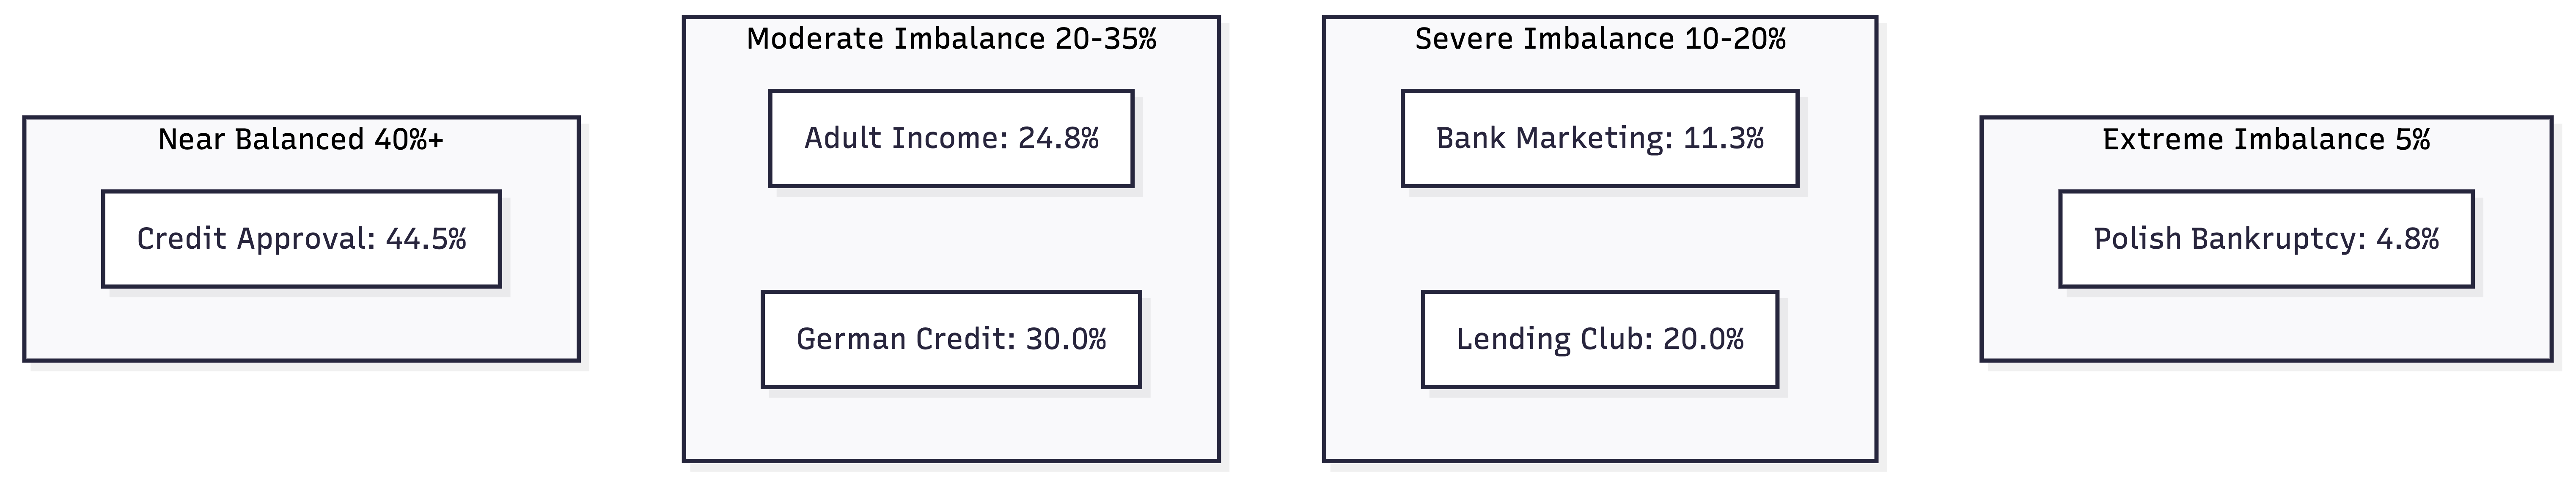
\includegraphics[width=\textwidth]{img/dataset_overview.png}
\caption{Overview of the six financial benchmark datasets used in this study, categorized by their class imbalance severity. Datasets range from near-balanced (Credit Approval at 44.5\%) to extreme imbalance (Polish Bankruptcy at 4.8\%).}
\label{fig:dataset_overview}
\end{figure}

Furthermore, tabular synthesis remains a significantly underexplored research area. Image synthesis has achieved remarkable results with models such as StyleGAN, DALL-E, and Stable Diffusion, as has text generation with GPT and LLaMA. Tabular synthesis lags significantly behind. Direct application of image-domain techniques fails on structured data, as we demonstrate empirically: TabDDPM \cite{kotelnikov2023tabddpm}, which applies diffusion directly to one-hot encoded tables, achieves KS statistics exceeding 0.80---indicating near-complete distributional mismatch. This failure occurs because one-hot encoded categorical features create sparse, discontinuous gradient landscapes that are incompatible with the smooth, continuous noise schedules used in standard diffusion processes.

Finally, tabular data underlies high-stakes decisions affecting individuals: loan approvals, insurance pricing, hiring recommendations, medical diagnoses. The quality of synthetic data directly impacts the fairness and accuracy of these decisions. A model trained on poorly synthesized data could systematically deny loans to qualified applicants or fail to flag fraudulent transactions, with material consequences for both consumers and institutions.

\section{Problem Statement and Research Gaps}
Despite significant progress in synthetic tabular data generation, a critical limitation persists: existing methods cannot control the class distribution of generated samples. This section examines the class imbalance problem in financial datasets, the limitations of current approaches, and the fundamental control gap that motivates this research.

\subsection{The class imbalance problem}
Financial datasets exhibit severe class imbalance, as documented across multiple benchmarks \cite{he2009imbalanced, chawla2002smote}:
\begin{itemize}
    \item Credit Card Fraud: Fraudulent transactions constitute only 0.1--0.5\% of the total.
    \item Loan Default: Defaulted loans represent 5--15\% of the portfolio.
    \item Company Bankruptcy: Only 3--8\% of companies in typical datasets are bankrupt.
    \item Suspicious Transactions (AML): Suspicious activity represents 0.01--1\% of all transactions.
\end{itemize}

Machine learning models trained on such data learn to predict the majority class, achieving high overall accuracy (e.g., 99\% by simply predicting ``not fraud'') while failing catastrophically on minority events---precisely the events of greatest business importance. This ``accuracy paradox'' means that standard evaluation metrics are misleading, and specialized metrics like minority-class F1-score, precision-recall AUC, and recall at fixed false-positive rates are essential.

\subsection{Limitations of existing approaches}
Traditional resampling methods have significant drawbacks:
\begin{itemize}
    \item SMOTE \cite{chawla2002smote} and its variants (Borderline-SMOTE, ADASYN) create interpolated samples that may lie outside the true data manifold, generating unrealistic feature combinations.
    \item Random undersampling discards valuable majority class information, reducing total training data and potentially removing important boundary examples.
    \item Neither approach generates truly novel samples; they merely redistribute or interpolate existing data points.
\end{itemize}

GAN-based methods such as CTGAN and TVAE also fall short:
\begin{itemize}
    \item Suffer from mode collapse \cite{salimans2016improved}, where the generator ``forgets'' minority modes of the distribution.
    \item Replicate the training class distribution without enhancement; generated data has the same imbalance as real data.
    \item No mechanism for post-hoc ratio adjustment---the user cannot request a specific minority ratio.
    \item Training instability makes reproducible results difficult to achieve.
\end{itemize}

Diffusion-based methods including TabDDPM and TabSyn present their own challenges:
\begin{itemize}
    \item TabDDPM \cite{kotelnikov2023tabddpm} fails on mixed-type data (KS $>$ 0.80), as direct diffusion on one-hot encoded features produces incoherent samples.
    \item TabSyn \cite{zhang2024tabsyn} achieves excellent fidelity (KS $\approx$ 0.10) by operating in a learned latent space but faithfully mirrors the training imbalance---if 5\% of training data is minority, approximately 5\% of synthetic data will also be minority.
    \item No existing diffusion-based method supports controllable class-conditional generation for tabular data.
\end{itemize}

\subsection{The control gap}
We identify a fundamental gap in the literature, confirmed through systematic review of 151 research papers across 10 categories:
\textit{No existing synthetic tabular data method enables practitioners to specify the desired class distribution during generation.}

This gap is particularly acute for financial applications, where balanced training data could significantly improve fraud detection, default prediction, and risk assessment. While Classifier-Free Guidance (CFG) \cite{ho2022cfg} has enabled remarkable control in image generation (enabling text-to-image models like Stable Diffusion \cite{rombach2022ldm} and DALL-E to produce highly specific outputs), its application to structured tabular data has remained entirely unexplored.

\section{Contributions}
This research makes the following contributions:

\textbf{1. Novel Application of Classifier-Free Guidance to Tabular Data.}
We introduce RE-TabSyn (Rare-Event Enhanced Tabular Synthesis), the first application of Classifier-Free Guidance (CFG) to tabular data synthesis. CFG, previously successful in image generation \cite{ho2022cfg}, enables controllable generation without auxiliary classifiers by jointly training conditional and unconditional models through a simple label dropout mechanism. This represents a fundamental advance in the tabular synthesis literature, opening a new research direction at the intersection of guided generation and structured data.

\textbf{2. Controllable Minority Class Generation.}
RE-TabSyn allows practitioners to specify target minority ratios via a single guidance scale parameter $w$. In our experiments, we boost minority representation from 4.8--44.5\% (original) to 44.8--50.2\% (generated), achieving near-balanced datasets on demand. This control is achieved at inference time without retraining the model, providing unmatched flexibility for downstream applications.

\textbf{3. Improved Minority Class Detection.}
We demonstrate that classifiers trained on RE-TabSyn synthetic data achieve a 3.1\% higher minority F1-score (0.472 vs.\ 0.458) than those trained on real imbalanced data---the first empirical evidence that guided synthetic data can outperform real data for minority detection tasks. This finding has profound implications for high-stakes applications where minority class detection is paramount.

\textbf{4. Comprehensive Financial Benchmark.}
We evaluate RE-TabSyn on six financial datasets spanning credit risk (German Credit, Credit Approval), income prediction (Adult Income), marketing response (Bank Marketing), loan performance (Lending Club), and corporate bankruptcy (Polish Bankruptcy). We provide systematic comparison against four baselines (CTGAN, TVAE, TabDDPM, TabSyn) across fidelity, utility, and privacy metrics, with statistical significance established across three random seeds (42, 123, 456).

\textbf{5. Conference Publication.}
The core findings of this research have been accepted for presentation at the \textbf{I2IT International Conference}, validating the scientific merit and novelty of the approach through external peer review. The paper titled ``\textit{Controllable Rare Event Synthetic Data Generation for Financial Tabular Data via Classifier Free Guidance}'' was accepted after rigorous review.

\section{Scope and Significance}
This section delineates the boundaries of the current research and articulates its practical, academic, and societal significance. The scope defines the specific problem domain and data characteristics addressed, while the significance highlights the broader impact across practice, research, and society.

\subsection{Scope}
This work addresses:
\begin{itemize}
    \item Binary classification tabular datasets with class imbalance (minority ratio from 4.8\% to 44.5\%).
    \item Single-table synthesis (relational/multi-table data is excluded from the current scope).
    \item Moderate dimensionality (tested on datasets with up to 64 features and up to 48,842 samples).
    \item Financial domain focus with broader applicability to healthcare, cybersecurity, and manufacturing.
\end{itemize}

\subsection{Significance}
RE-TabSyn enables financial institutions to:
\begin{itemize}
    \item Train more effective fraud detection models by generating balanced training data with realistic minority samples.
    \item Conduct bias auditing with balanced synthetic data across demographic groups without access to real protected-class data.
    \item Share data across organizational boundaries safely, enabling federated analytics without data exposure.
    \item Augment rare event datasets for improved stress testing and regulatory compliance.
\end{itemize}

From a research perspective, this work:
\begin{itemize}
    \item Bridges controllable image generation techniques (CFG) to the tabular domain for the first time.
    \item Establishes benchmarks for minority-aware synthetic data evaluation beyond simple fidelity metrics.
    \item Opens research directions in guided tabular synthesis, including multi-class control, continuous attribute conditioning, and privacy-guided generation.
\end{itemize}

Improved minority class detection directly benefits society:
\begin{itemize}
    \item \textbf{Consumers:} Better fraud protection, fairer credit decisions, and reduced false rejections.
    \item \textbf{Financial Institutions:} Reduced fraud losses, better risk models, and regulatory compliance.
    \item \textbf{Regulators:} Enhanced oversight capability through synthetic benchmarks for stress testing and fairness auditing.
\end{itemize}

\section{Organization of the Report}
The remainder of this report is organized as follows:
\begin{itemize}
    \item \textbf{Chapter 2: Research Analysis and Methodology} presents the formal problem formulation, mathematical foundations of baseline methods, and the detailed architecture and theoretical analysis of the proposed RE-TabSyn framework.
    \item \textbf{Chapter 3: Literature Review} surveys 151 peer-reviewed publications across generative models, tabular synthesis, privacy-preserving mechanisms, and evaluation frameworks, culminating in a gap analysis that motivates our approach.
    \item \textbf{Chapter 4: Implementation and Experimental Setup} describes the end-to-end pipeline, data preprocessing, model configurations, training procedures, and evaluation protocols.
    \item \textbf{Chapter 5: Research Outcomes} presents comprehensive results across fidelity, utility, privacy, and minority control metrics, with statistical significance analysis.
    \item \textbf{Chapter 6: Conclusion} summarizes key findings, discusses limitations, and presents concluding remarks.
    \item \textbf{Chapter 7: Future Scope} outlines promising research directions including architectural improvements, differential privacy integration, and extended synthesis capabilities.
\end{itemize}

\flushbottom
%%-------------------------------------------------------------------------
\flushbottom
\chapter{Research Analysis and Methodology}

This chapter presents the formal mathematical foundations of the proposed RE-TabSyn framework, beginning with the problem formulation, proceeding through the theoretical basis of each baseline method, and culminating in a detailed description of our three-component architecture with accompanying theoretical analysis.

\section{Problem Formulation}

Let $\mathcal{D} = \{(\mathbf{x}_i, y_i)\}_{i=1}^{N}$ denote a tabular dataset where $\mathbf{x}_i \in \mathcal{X}$ represents a feature vector and $y_i \in \{0, 1\}$ denotes the class label.

Each feature vector comprises numerical and categorical attributes:
\begin{equation}
\mathbf{x} = (\mathbf{x}^{(num)}, \mathbf{x}^{(cat)}) \in \mathbb{R}^{d_{num}} \times \prod_{j=1}^{d_{cat}} \mathcal{C}_j
\end{equation}
where $\mathcal{C}_j$ is the categorical domain for attribute $j$ with cardinality $|\mathcal{C}_j|$.

The class imbalance is quantified by the minority ratio $\rho = N_1 / N$, where $N_1 = |\{i : y_i = 1\}|$ is the minority class count. In our benchmark datasets, $\rho$ ranges from 0.048 to 0.445.

The core learning objective is: learn a generative model $G_\theta$ that synthesizes samples $\tilde{\mathbf{x}} \sim p_\theta(\mathbf{x})$ indistinguishable from $\mathbf{x} \sim p_{data}(\mathbf{x})$, with the additional capability to control the class distribution $p_\theta(y)$ at generation time. This is a stricter objective than standard generative modeling: the target is samples whose class composition can be specified by the user after training, not merely realistic samples. Four criteria guide the framework design:
\begin{enumerate}
    \item Fidelity: $p_\theta(\mathbf{x}) \approx p_{data}(\mathbf{x})$ (distributional similarity), measured by the Kolmogorov-Smirnov, i.e., KS, statistic, where lower values indicate better fidelity.

    \item Utility: Classifiers trained on synthetic data perform comparably to those trained on real data, measured via the Train-on-Synthetic Test-on-Real, i.e., TSTR, protocol using AUC-ROC and F1-score.

    \item Privacy: Synthetic samples do not memorize training instances, measured by Distance to Closest Record, i.e., DCR, where higher values indicate stronger privacy.

    \item Controllability: User-specified class ratio $\pi = P(y=1)$ achievable without model retraining, measured by the deviation between target and achieved minority ratios.
\end{enumerate}

No previous method satisfies all four desiderata simultaneously. TabSyn satisfies the first three but not the fourth. CTGAN partially satisfies fidelity and utility but fails on privacy (weak DCR) and completely fails on controllability. RE-TabSyn is designed to satisfy all four, accepting a modest fidelity cost relative to TabSyn as the price of gaining controllability.

\section{Baseline Methods: Theoretical Foundations}

This section provides the mathematical foundations of the four baseline methods against which RE-TabSyn is evaluated; each method's limitations motivate specific design choices in the proposed approach.

\subsection{Generative adversarial networks (GANs)}

GANs \cite{goodfellow2014gan} formulate generative modeling as a two-player minimax game between a generator $G$ and discriminator $D$:
\begin{equation}
\min_G \max_D \mathcal{L}_{GAN}(G, D) = \mathbb{E}_{\mathbf{x} \sim p_{data}}[\log D(\mathbf{x})] + \mathbb{E}_{\mathbf{z} \sim p_z}[\log(1 - D(G(\mathbf{z})))]
\end{equation}

Training dynamics are notoriously unstable: a discriminator that is too strong causes vanishing gradients for $G$, while one that is too weak provides no learning signal. Techniques such as Wasserstein distance \cite{arjovsky2017wgan} and spectral normalization help, but do not fully resolve the problem.

CTGAN \cite{xu2019ctgan} extends vanilla GANs for tabular data through two innovations:
\begin{enumerate}
    \item Mode-specific normalization: numerical columns are modeled as mixtures of Gaussians via VGMMs, allowing the transform to adapt to multimodal distributions rather than assuming unimodal structure.

    \item Conditional generator with training-by-sampling: a conditional vector specifies which categorical value to generate, and training oversamples rare categories.
\end{enumerate}

Despite these innovations, CTGAN suffers from mode collapse on minority classes: the generator may ``forget'' rare modes because the gradient signal from minority samples is overwhelmed by the majority class signal. CTGAN also provides no mechanism for post-hoc ratio adjustment; the generated data mirrors the training distribution. In experiments on the Polish Bankruptcy dataset (4.8\% minority), CTGAN achieves a minority F1-score of just 0.112, barely above random guessing, confirming that mode collapse on extreme minority classes is a practical failure, not merely a theoretical concern.

\subsection{Variational autoencoders}

VAEs \cite{kingma2014vae} model data through latent variables $\mathbf{z}$ using variational inference. The core idea: instead of directly modeling the complicated high-dimensional data distribution $p(\mathbf{x})$, introduce a simpler latent variable $\mathbf{z}$ and model the joint distribution $p(\mathbf{x}, \mathbf{z})$. Generation then proceeds by first sampling $\mathbf{z} \sim p(\mathbf{z})$ from the simple prior (a standard Gaussian) and then decoding $\mathbf{x} \sim p_\theta(\mathbf{x}|\mathbf{z})$.

The generative model defines a joint distribution $p_\theta(\mathbf{x}, \mathbf{z}) = p_\theta(\mathbf{x}|\mathbf{z}) p(\mathbf{z})$, where $p(\mathbf{z}) = \mathcal{N}(\mathbf{0}, \mathbf{I})$ is a standard Gaussian prior. Since the true posterior is intractable, an approximate posterior $q_\phi(\mathbf{z}|\mathbf{x})$ is introduced. The Evidence Lower Bound, i.e., ELBO, provides a tractable training objective:
\begin{equation}
\log p_\theta(\mathbf{x}) \geq \underbrace{\mathbb{E}_{q_\phi(\mathbf{z}|\mathbf{x})}[\log p_\theta(\mathbf{x}|\mathbf{z})]}_{\text{Reconstruction Term}} - \underbrace{D_{KL}(q_\phi(\mathbf{z}|\mathbf{x}) \parallel p(\mathbf{z}))}_{\text{Regularization Term}}
\end{equation}

The reconstruction term encourages the encoder to produce informative latent codes. The KL term regularizes the posterior toward the Gaussian prior.

The reparameterization trick $\mathbf{z} = \boldsymbol{\mu} + \boldsymbol{\sigma} \odot \boldsymbol{\epsilon}$, where $\boldsymbol{\epsilon} \sim \mathcal{N}(\mathbf{0}, \mathbf{I})$, enables end-to-end gradient-based optimization.

TVAE applies VAE principles to tabular data with mixed-type reconstruction losses (MSE for numerical features, cross-entropy for categorical features) but has three limitations. First, the Gaussian likelihood assumption produces blurry reconstructions that average over modes rather than capturing them sharply, potentially generating unrealistic in-between samples. Second, in high-dimensional settings the KL term can dominate training, causing posterior collapse where the decoder learns to reconstruct without using the latent code. Third, TVAE has no class conditioning mechanism, preventing controlled generation.

RE-TabSyn addresses these limitations by using a $\beta$-VAE formulation ($\beta = 0.1$, weighting the KL term down) to prevent posterior collapse while maintaining smooth latent geometry, and by adding class conditioning through the downstream diffusion model rather than into the VAE itself.

\subsection{Diffusion models}

Diffusion models \cite{ho2020ddpm} define a forward noising process that gradually destroys data structure, and then learn to reverse it. The intuition is straightforward: if you know how data is destroyed, you can learn to reconstruct it.

The forward process is a Markov chain that adds Gaussian noise over $T$ timesteps according to a variance schedule $\{\beta_t\}_{t=1}^{T}$:
\begin{equation}
q(\mathbf{z}_t | \mathbf{z}_{t-1}) = \mathcal{N}(\mathbf{z}_t; \sqrt{1-\beta_t}\,\mathbf{z}_{t-1}, \beta_t \mathbf{I})
\end{equation}

A useful property enables direct sampling of any timestep $t$ without iterating through all previous steps:
\begin{equation}
q(\mathbf{z}_t | \mathbf{z}_0) = \mathcal{N}(\mathbf{z}_t; \sqrt{\bar{\alpha}_t}\,\mathbf{z}_0, (1-\bar{\alpha}_t)\mathbf{I})
\end{equation}
where $\alpha_t = 1 - \beta_t$ and $\bar{\alpha}_t = \prod_{s=1}^{t} \alpha_s$.

The reverse process learns to denoise by predicting the noise $\epsilon_\theta(\mathbf{z}_t, t)$ added at each step, trained with a simple MSE objective:
\begin{equation}
\mathcal{L}_{simple} = \mathbb{E}_{t, \mathbf{z}_0, \boldsymbol{\epsilon}} \left[ \|\boldsymbol{\epsilon} - \epsilon_\theta(\mathbf{z}_t, t)\|^2 \right]
\end{equation}

\begin{figure}[H]
\centering

\includegraphics[width=\textwidth]{img/diffusion_chain.png}
\caption{Forward and reverse diffusion process.}
\label{fig:diffusion_chain}
\end{figure}

TabDDPM \cite{kotelnikov2023tabddpm} was the first systematic application of diffusion to tabular data. It treats numerical features with Gaussian diffusion and categorical features with multinomial diffusion. However, it demonstrates poor performance on mixed-type data because direct diffusion on one-hot encoded categorical features creates sparse, discontinuous gradients. To see why: a one-hot vector like $[0, 0, 1, 0]$ has most values at exactly zero. Adding Gaussian noise produces a dense vector like $[0.05, -0.12, 0.88, 0.03]$ that does not correspond to any valid category. The model must denoise vectors it has never seen in training data, creating a mismatch between the training distribution and the inference distribution. Our experiments confirm this failure: TabDDPM achieves an average KS statistic of 0.770, indicating near-complete distributional mismatch.

TabSyn \cite{zhang2024tabsyn} addresses TabDDPM's limitations by performing diffusion in a learned latent space. A VAE first encodes mixed-type tabular data into continuous representations where diffusion operates effectively. The discrete categorical values are absorbed into the continuous latent space by the VAE encoder, so the diffusion model only ever sees continuous vectors. A Transformer backbone then captures inter-column dependencies, achieving the best reported tabular fidelity at the time with an average KS of 0.109. However, TabSyn lacks any mechanism for controlling class distribution and cannot address class imbalance explicitly.

\section{Proposed Method: RE-TabSyn}

RE-TabSyn (Rare-Event Enhanced Tabular Synthesis) combines three interlocking components to achieve both fidelity and controllable minority generation. The complete system architecture is illustrated in Figure~\ref{fig:system_architecture}.

\begin{figure}[H]
\centering
\includegraphics[width=\textwidth]{img/system_architecture.png}
\caption{RE-TabSyn five-module system architecture.}
\label{fig:system_architecture}
\end{figure}

The three core components are:
\begin{enumerate}
    \item Variational Autoencoder (VAE) --- mixed-type encoding into continuous latent space
    \item Latent Diffusion Model (LDM) --- generation in the smooth continuous latent space
    \item Classifier-Free Guidance (CFG) --- controllable class ratios at inference time
\end{enumerate}

The three components are not independently useful; they work because of how they interact. The VAE solves the encoding problem so that the diffusion model operates in a well-behaved continuous space. The diffusion model learns a powerful generative model of that space. And the CFG mechanism uses the diffusion model's conditioning architecture to steer generation toward the desired class. Remove any one component and the system breaks: without the VAE, diffusion fails on categorical features; without the diffusion model, there is no way to apply CFG; without CFG, class control is impossible.

\subsection{Component 1: Tabular VAE}

The VAE is the foundation of RE-TabSyn, solving the critical problem of encoding heterogeneous tabular data into a smooth, continuous latent space where diffusion can operate effectively. The architecture is illustrated in Figure~\ref{fig:vae_architecture}.

\begin{figure}[H]
\centering
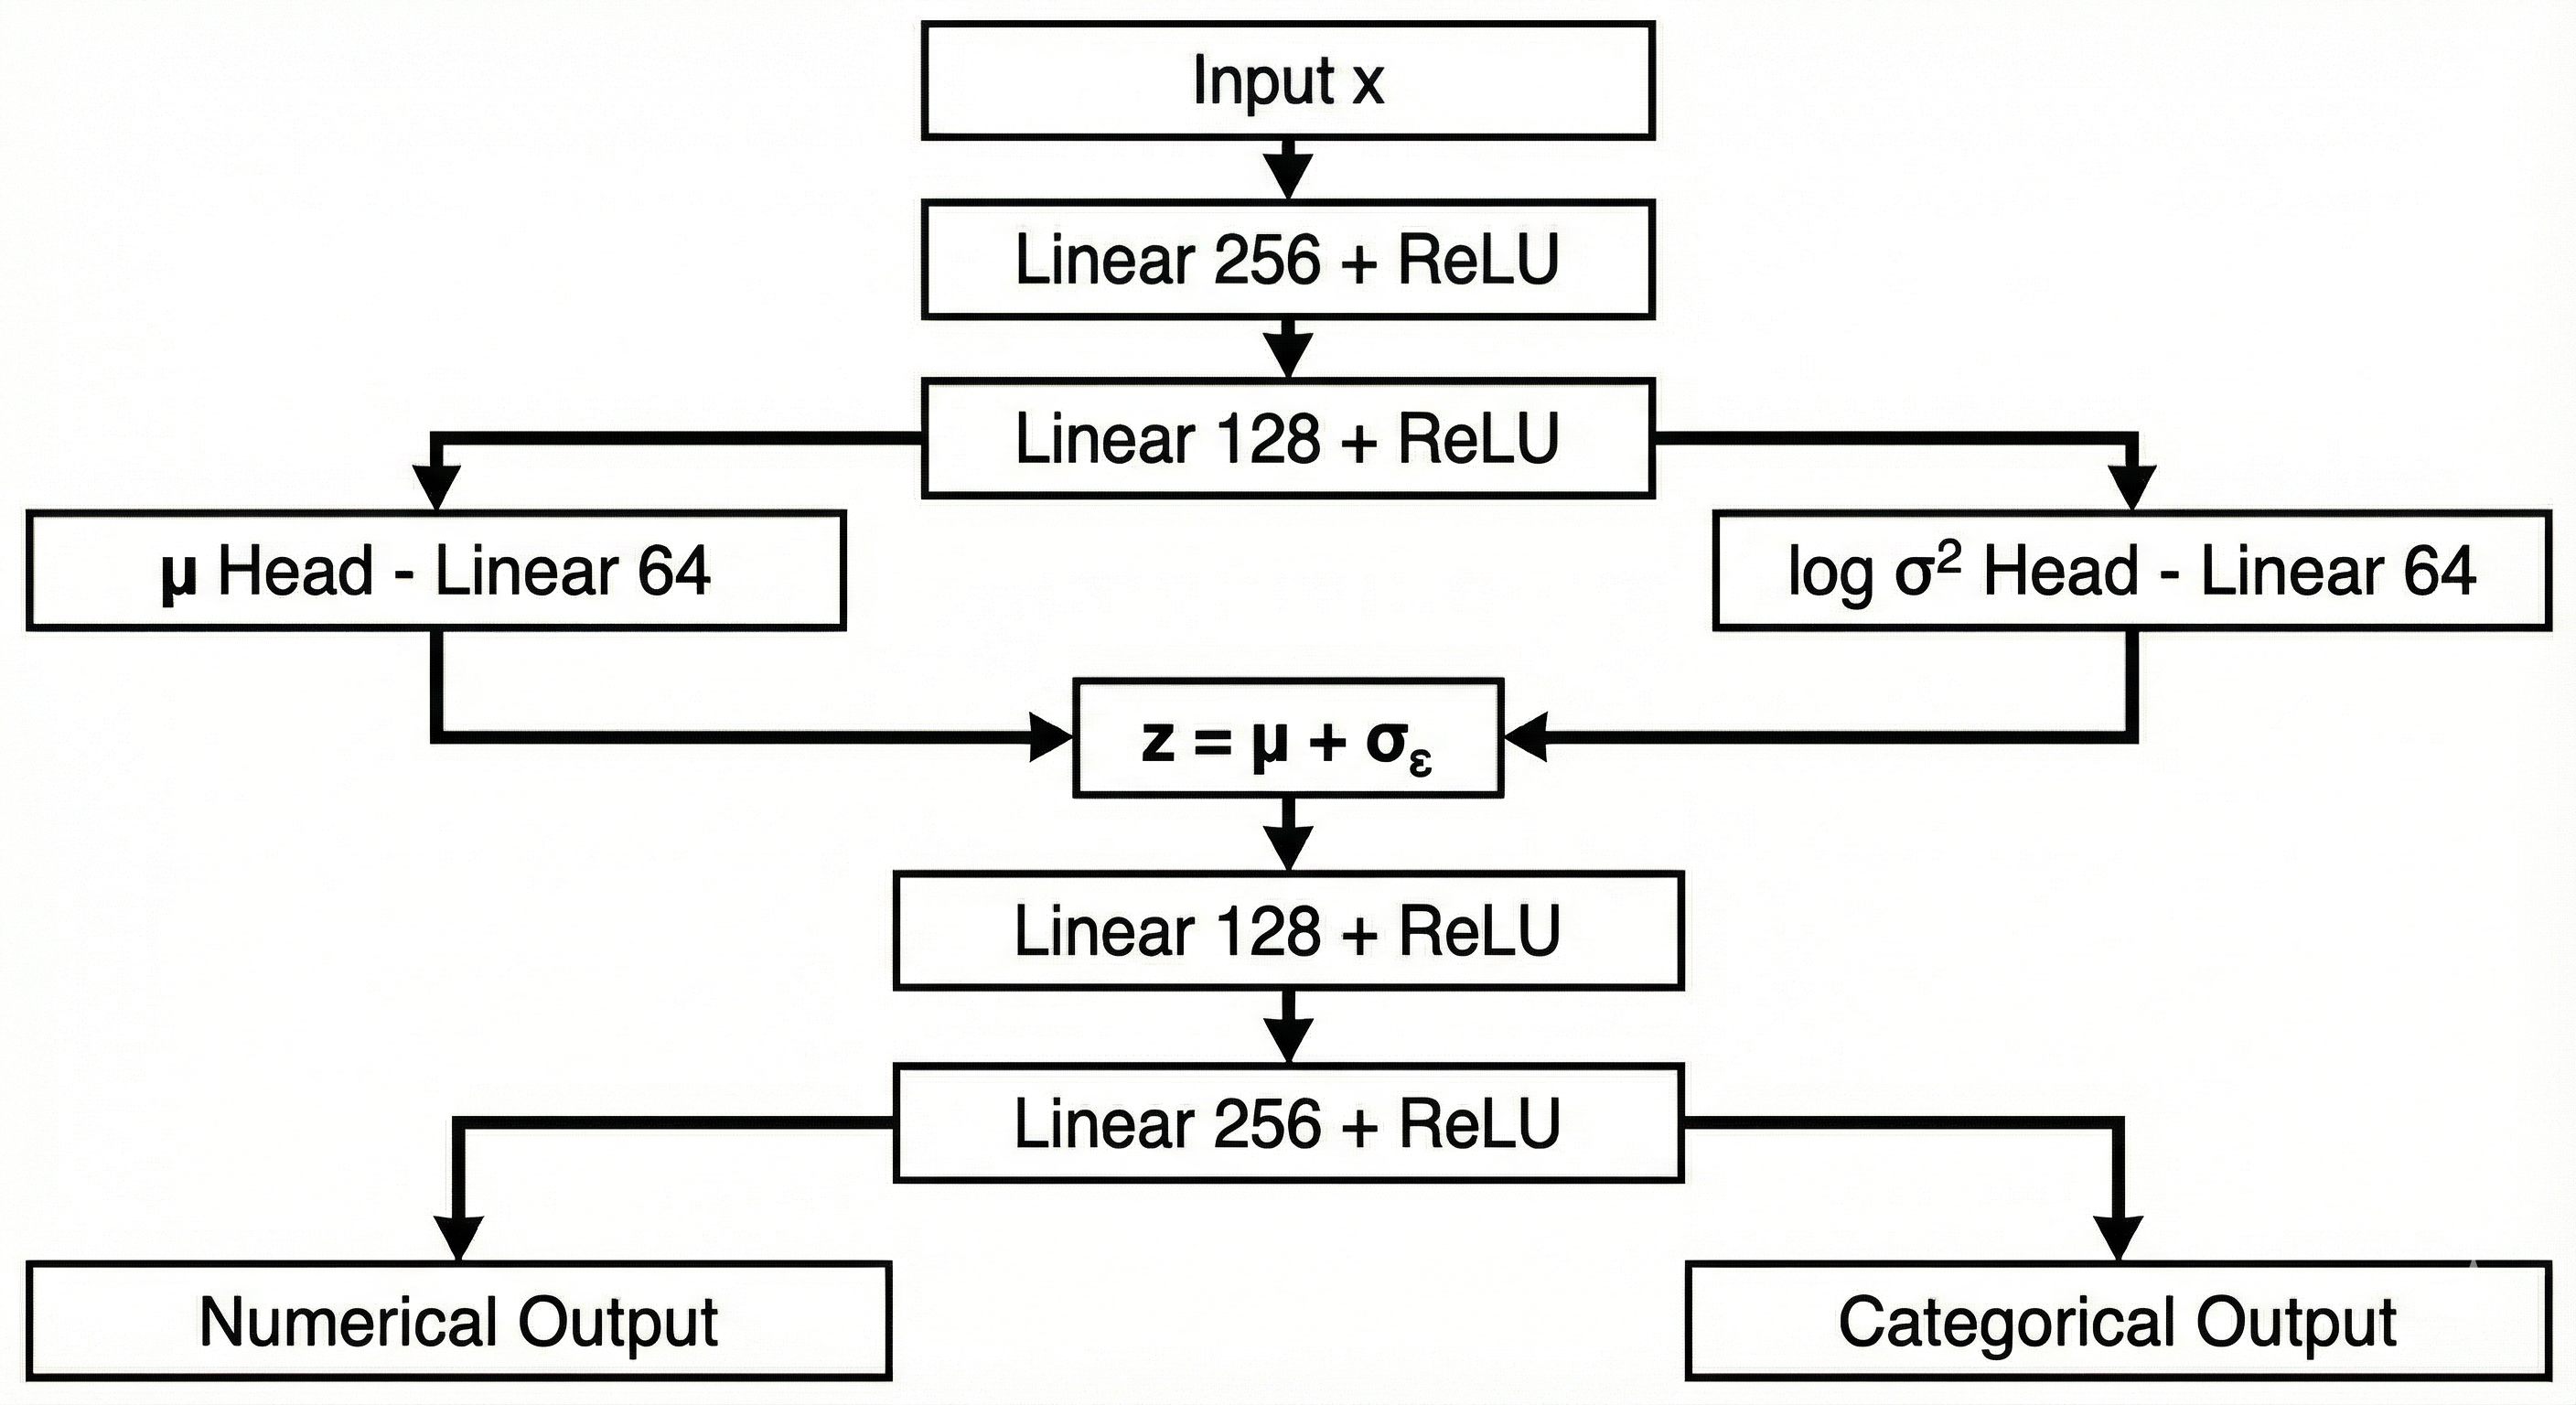
\includegraphics[width=0.85\textwidth]{img/vae_architecture.png}
\caption{Tabular VAE encoder-decoder architecture.}
\label{fig:vae_architecture}
\end{figure}

The encoder maps mixed-type input $\mathbf{x} \in \mathbb{R}^{d}$ to latent parameters $(\boldsymbol{\mu}, \log \boldsymbol{\sigma}^2)$ through an MLP with hidden dimensions (256, 128):
\begin{equation}
\boldsymbol{\mu}, \log \boldsymbol{\sigma}^2 = \text{Encoder}_\phi(\mathbf{x}) \quad \text{where} \quad \boldsymbol{\mu}, \log \boldsymbol{\sigma}^2 \in \mathbb{R}^{64}
\end{equation}

The latent variable is sampled via the reparameterization trick:
\begin{equation}
\mathbf{z} = \boldsymbol{\mu} + \boldsymbol{\sigma} \odot \boldsymbol{\epsilon}, \quad \boldsymbol{\epsilon} \sim \mathcal{N}(\mathbf{0}, \mathbf{I})
\end{equation}

Here, $\boldsymbol{\sigma} = \exp(\frac{1}{2} \log \boldsymbol{\sigma}^2)$ (computed element-wise), and $\odot$ denotes element-wise multiplication.

The decoder reconstructs from the latent code, utilizing separate loss functions for different feature types:
\begin{equation}
\mathcal{L}_{VAE} = \underbrace{\sum_{j=1}^{d_{num}} \|\mathbf{x}_j - \hat{\mathbf{x}}_j\|^2}_{\text{Numerical MSE}} + \underbrace{\sum_{j=1}^{d_{cat}} \text{CE}(\mathbf{x}_j, \hat{\mathbf{x}}_j)}_{\text{Categorical Cross-Entropy}} + \underbrace{\beta \cdot D_{KL}(q_\phi(\mathbf{z}|\mathbf{x}) \parallel p(\mathbf{z}))}_{\text{KL Regularization}}
\end{equation}
where $\beta = 0.1$ balances reconstruction quality and latent space regularization.

MSE is used for numerical features and cross-entropy for categorical features, since MSE is inappropriate for discrete class labels. $\beta = 0.1$ prevents posterior collapse while maintaining sufficient latent space regularity.

\subsection{Component 2: Latent diffusion model}

Given the encoded latent representation $\mathbf{z}_0 = \text{Encoder}_\phi(\mathbf{x})$, the forward diffusion process adds noise according to a linear schedule with $T = 1000$ timesteps, $\beta_1 = 10^{-4}$, and $\beta_T = 0.02$.

We employ a Diffusion Transformer (DiT) \cite{peebles2023dit} architecture for the noise prediction network, chosen for its ability to capture inter-feature dependencies through self-attention:
\begin{equation}
\epsilon_\theta(\mathbf{z}_t, t, y) = \text{DiT}(\mathbf{z}_t, \text{TimeEmb}(t), \text{ClassEmb}(y))
\end{equation}

The DiT architecture consists of:
\begin{enumerate}
    \item 4 Transformer layers with self-attention and feed-forward blocks.

    \item Hidden dimension of 256 with 4 attention heads (64 dimensions per head).

    \item Sinusoidal time embeddings projected through an MLP to match the hidden dimension.

    \item Learned class embeddings for the binary label (class 0, class 1, and null token $\emptyset$).

    \item Adaptive Layer Normalization (AdaLN) \cite{ba2016layernorm} conditioning each transformer block on the sum of time and class embeddings.
\end{enumerate}

\begin{figure}[H]
\centering
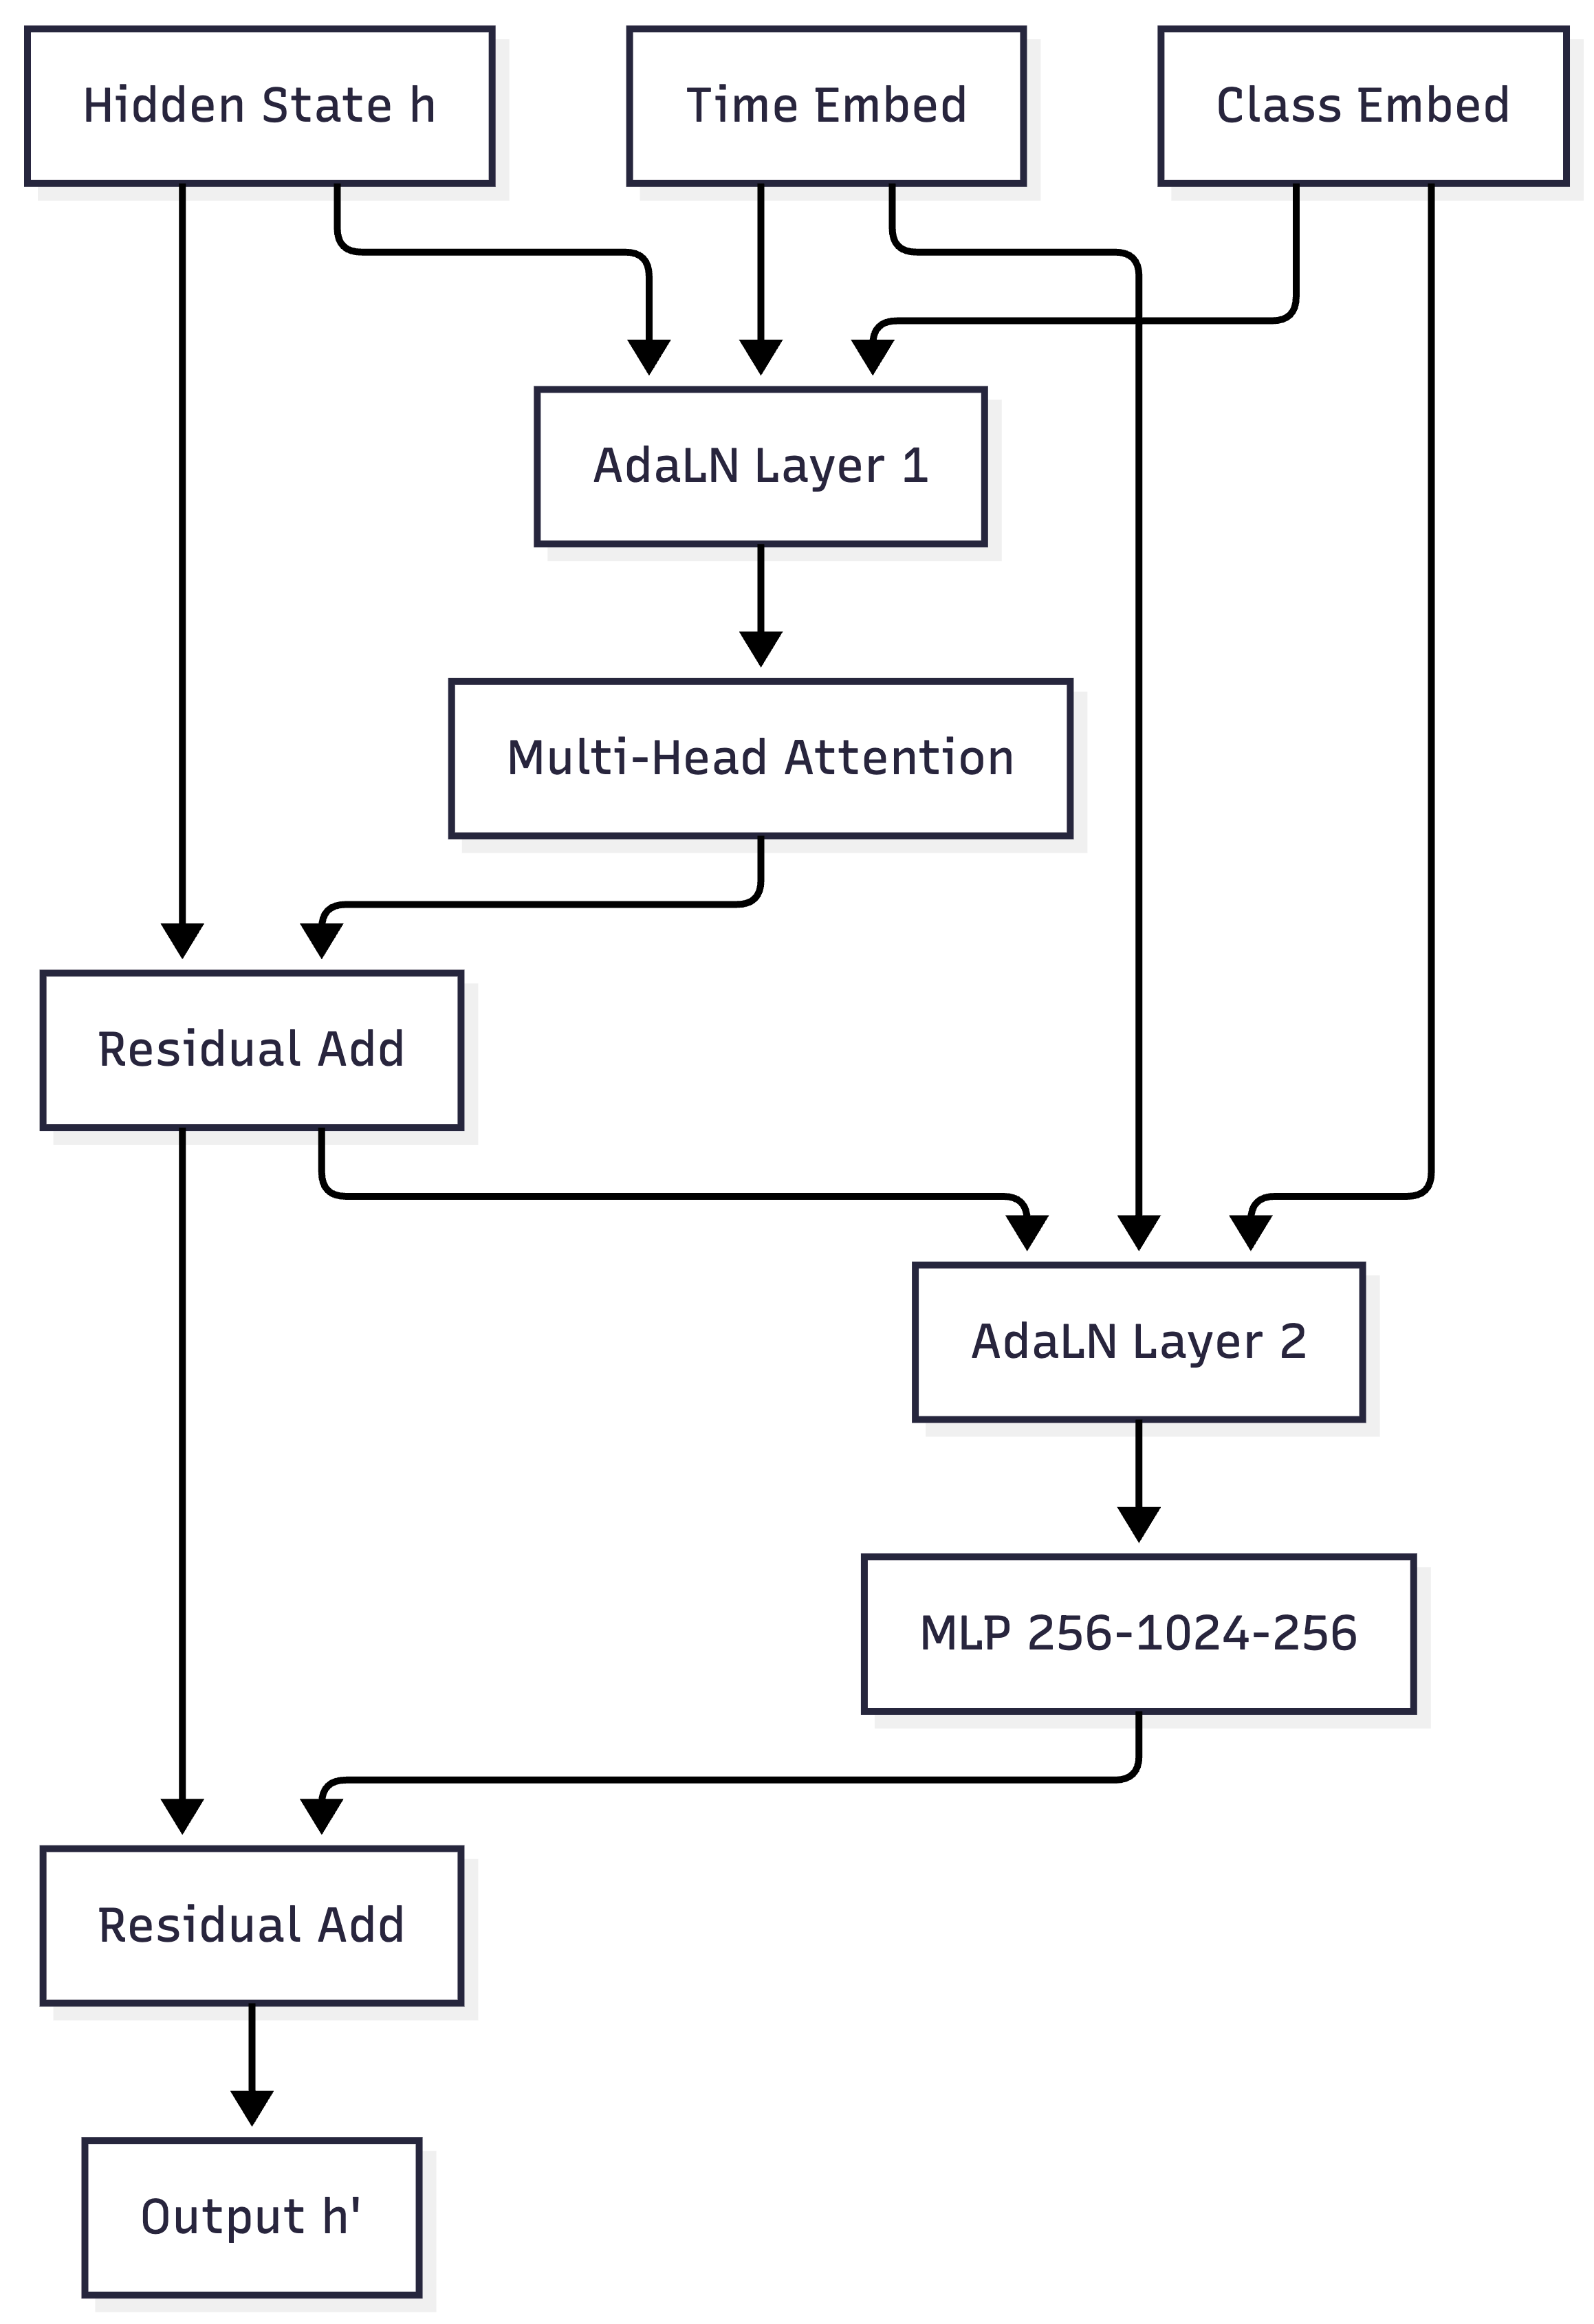
\includegraphics[width=0.45\textwidth]{img/dit_block.png}
\caption{Single DiT block with AdaLN conditioning.}
\label{fig:dit_block}
\end{figure}

The training objective minimizes the expected squared error between the true noise and the predicted noise:
\begin{equation}
\mathcal{L}_{diff} = \mathbb{E}_{t \sim \mathcal{U}(1,T),\, \mathbf{z}_0,\, \boldsymbol{\epsilon} \sim \mathcal{N}(\mathbf{0}, \mathbf{I})} \left[ \|\boldsymbol{\epsilon} - \epsilon_\theta(\sqrt{\bar{\alpha}_t}\,\mathbf{z}_0 + \sqrt{1-\bar{\alpha}_t}\,\boldsymbol{\epsilon},\, t,\, y)\|^2 \right]
\end{equation}

\subsection{Component 3: Classifier-free guidance}

Classifier-Free Guidance \cite{ho2022cfg} enables controllable generation in RE-TabSyn. The mechanism is illustrated in Figure~\ref{fig:cfg_mechanism}.

\begin{figure}[H]
\centering
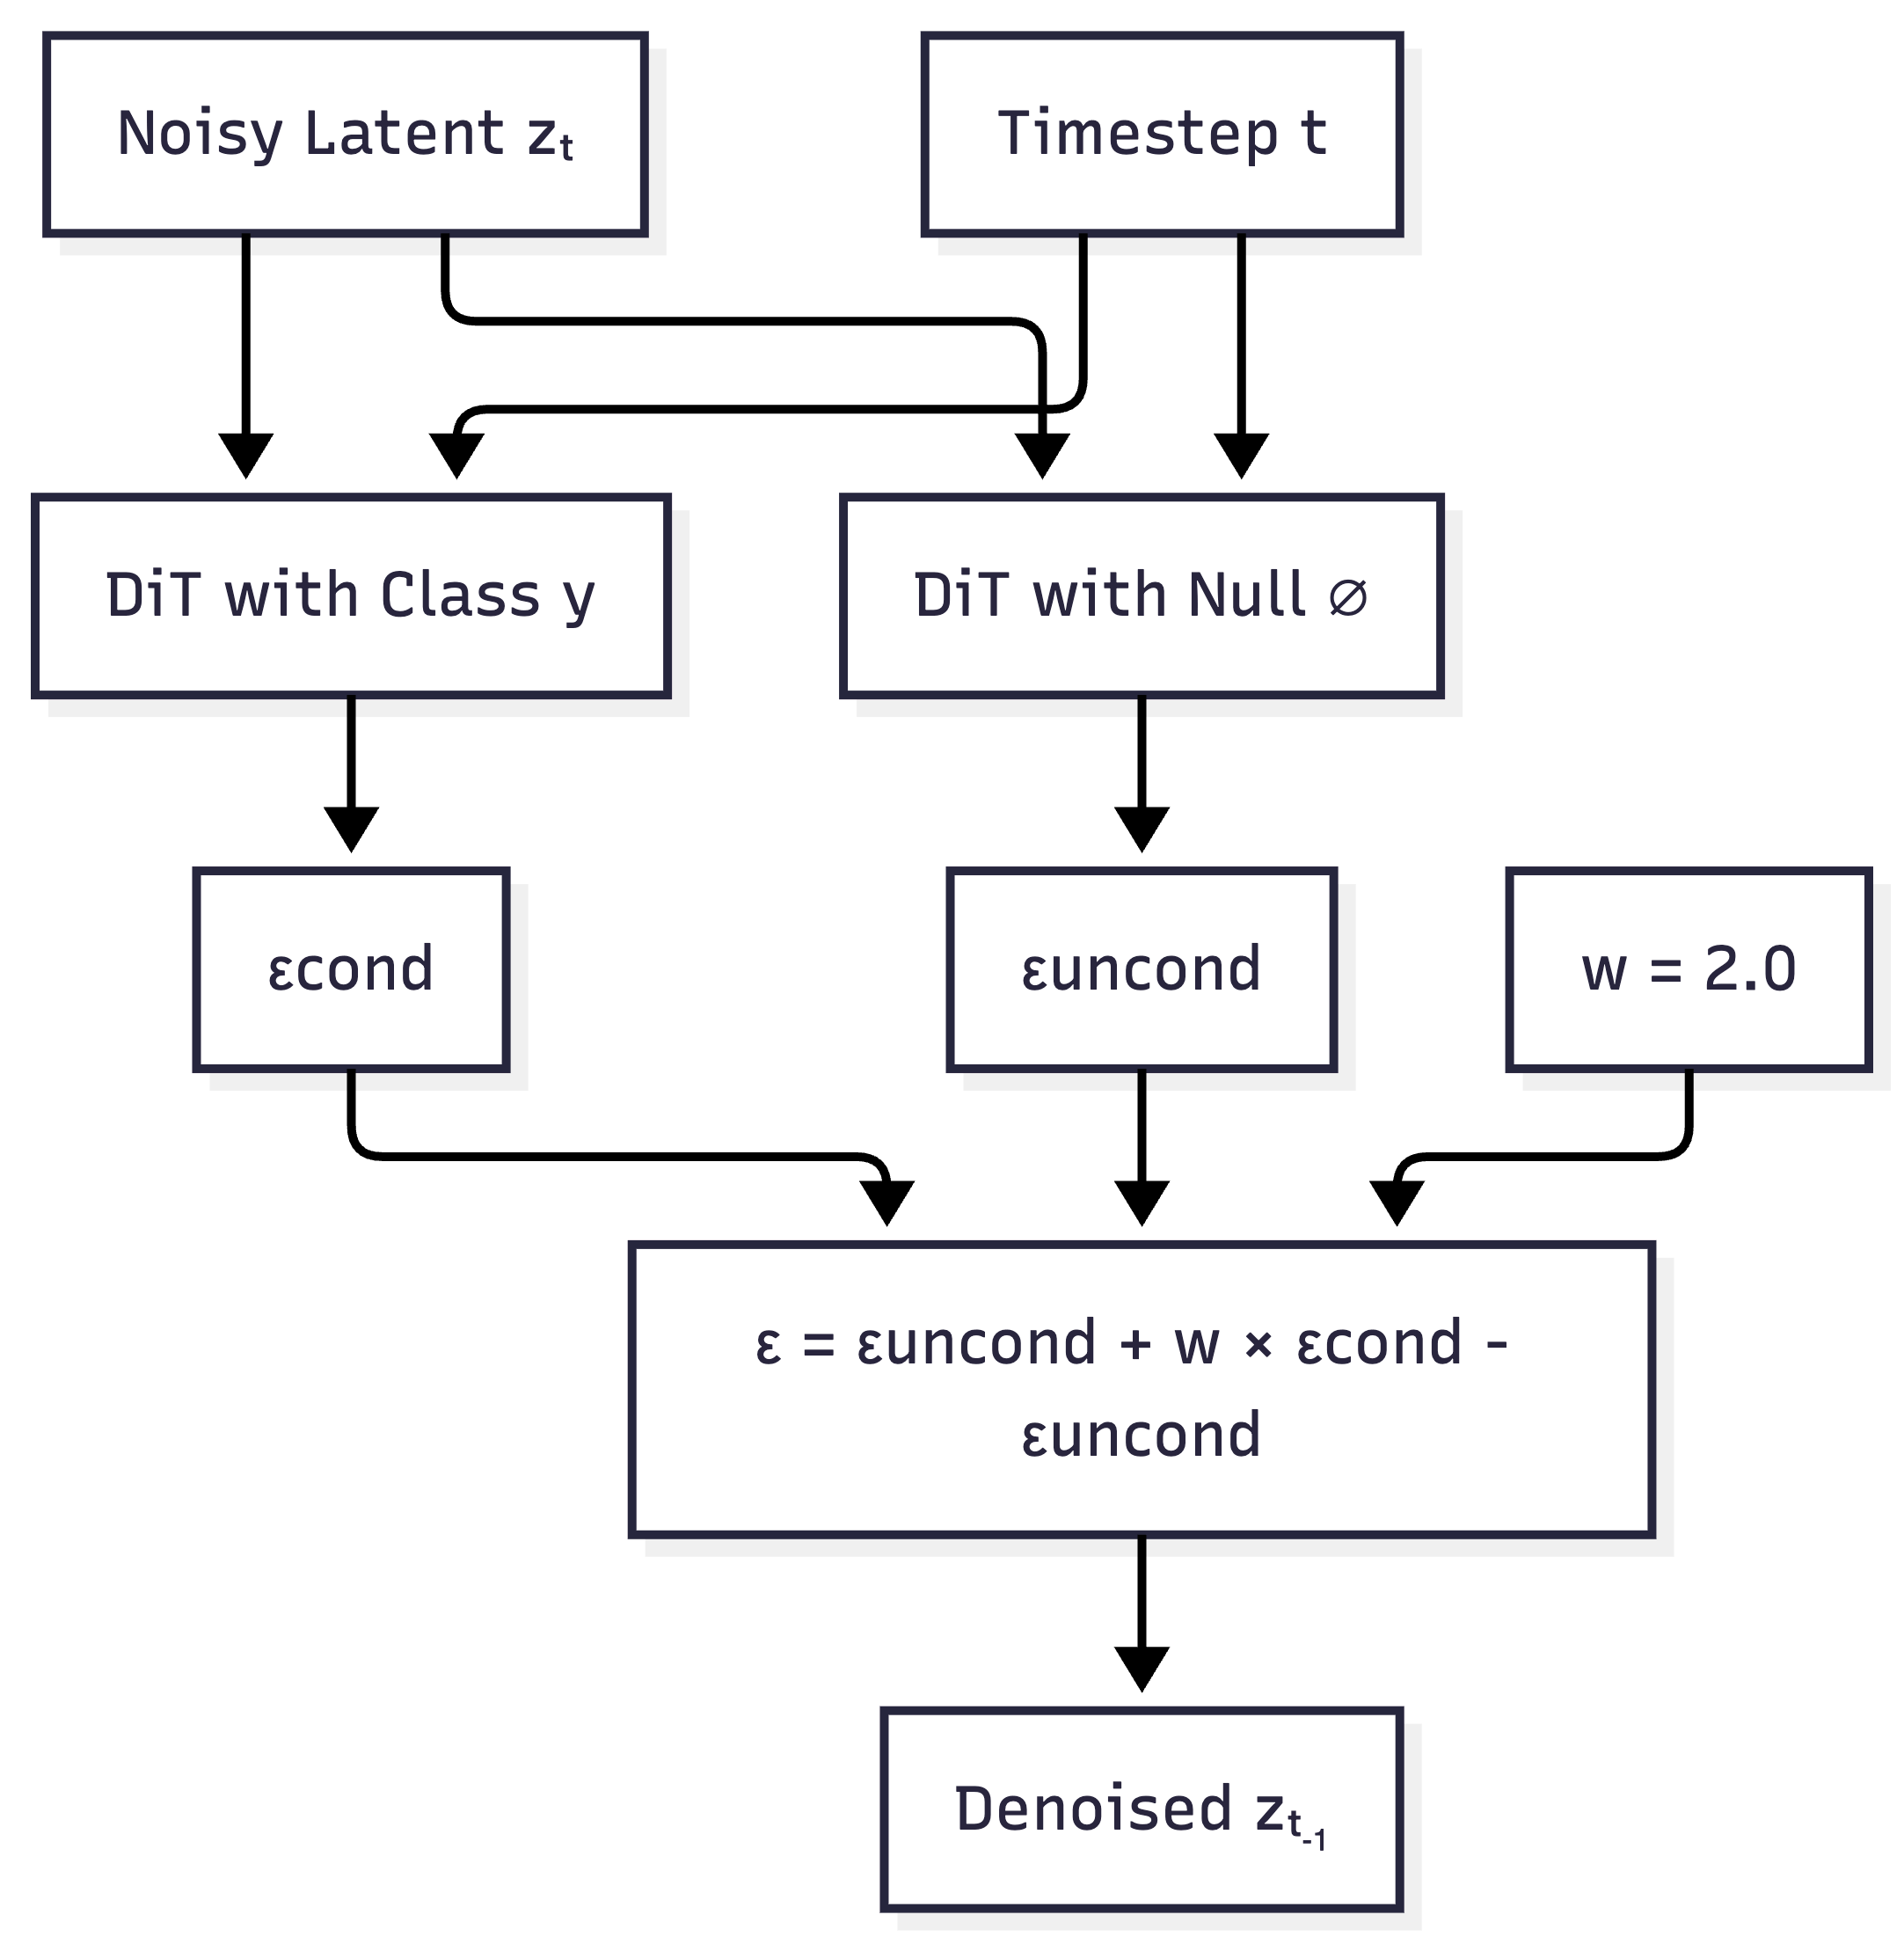
\includegraphics[width=0.7\textwidth]{img/cfg_mechanism.png}
\caption{CFG inference: two DiT passes blended.}
\label{fig:cfg_mechanism}
\end{figure}

During training, class labels are randomly replaced with a null token $\emptyset$ with probability $p_{uncond} = 0.10$, following the recommendation \cite{ho2022cfg}.

\begin{figure}[H]
\centering
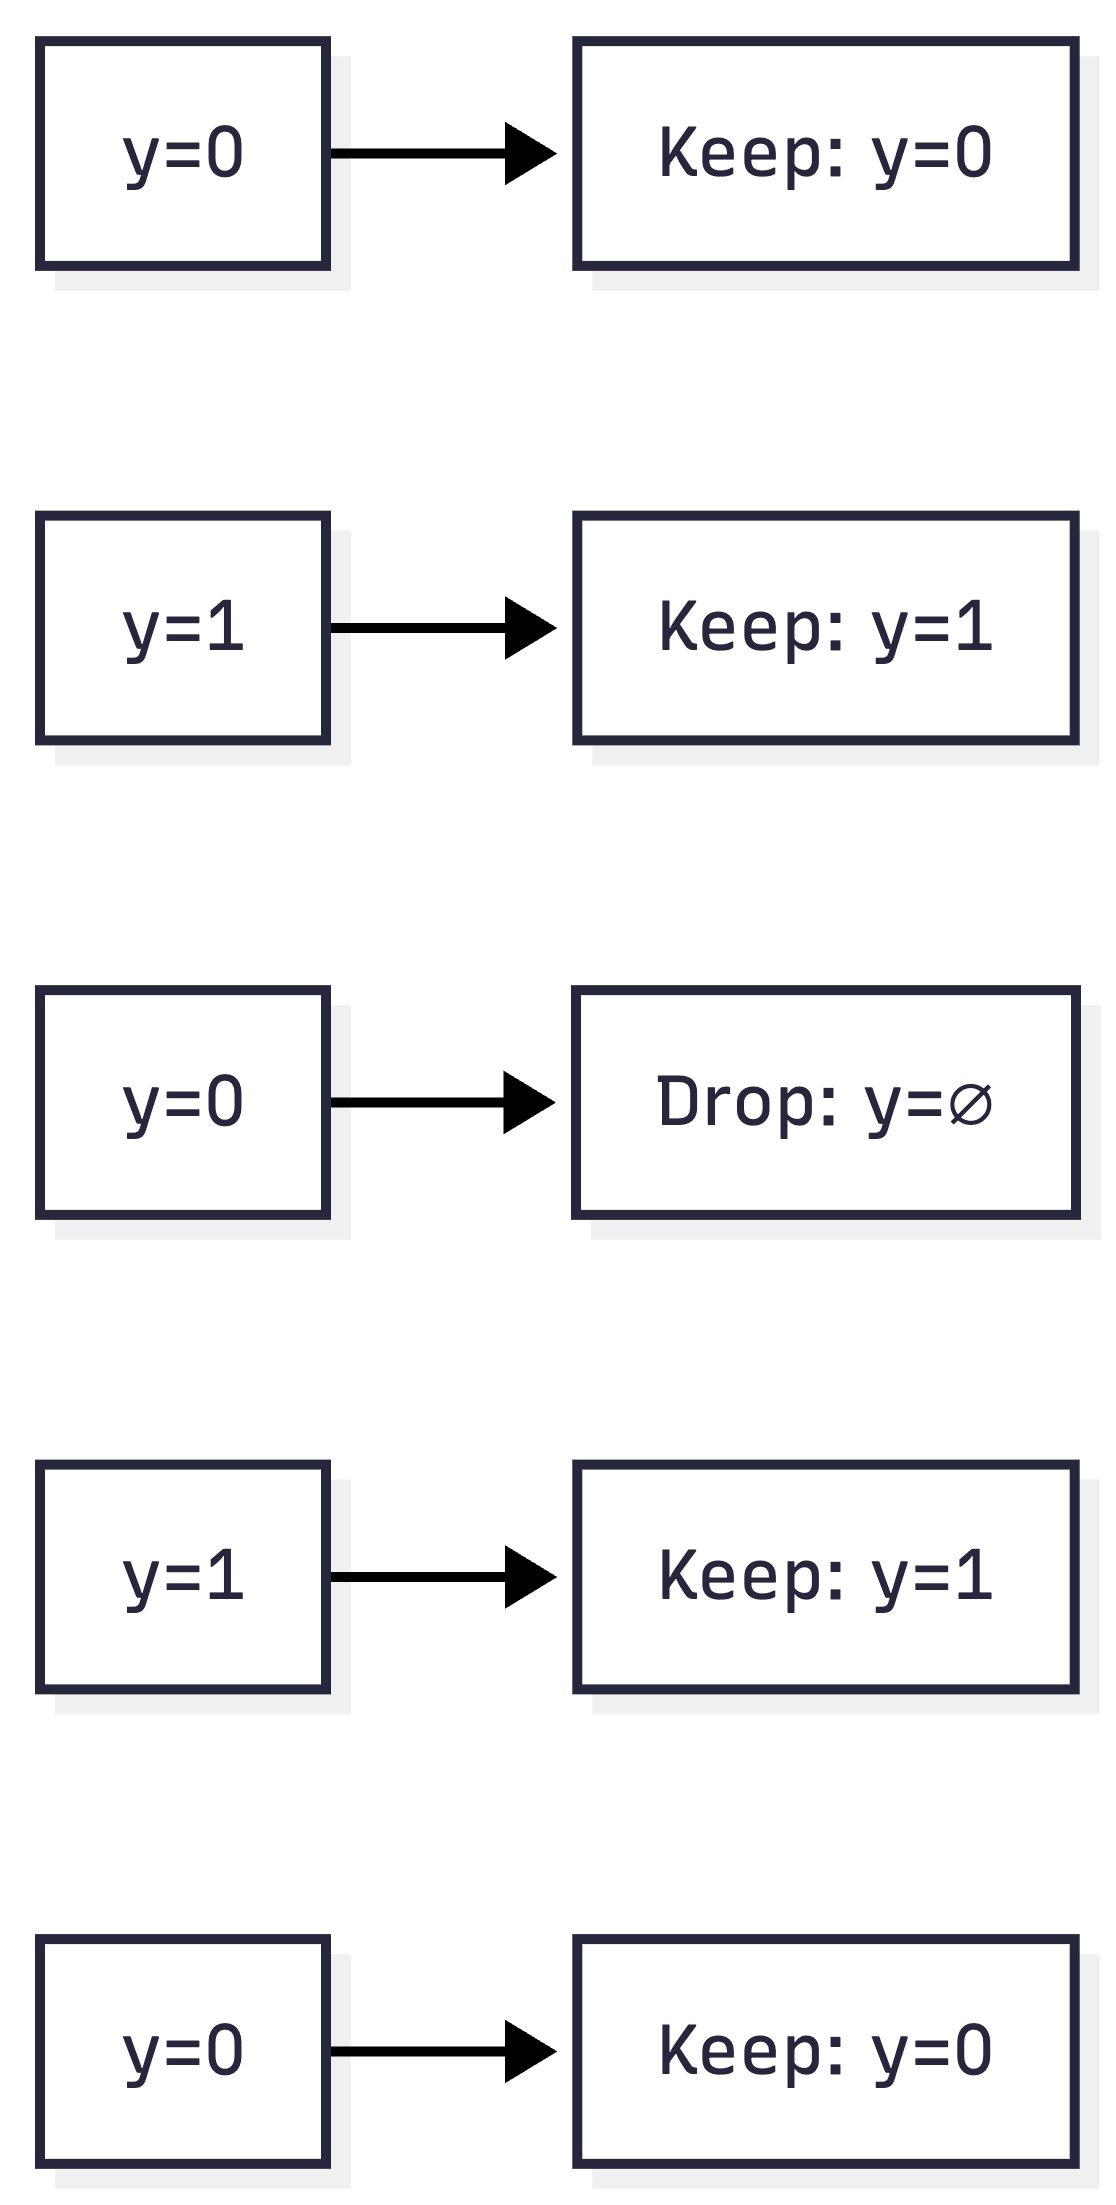
\includegraphics[width=0.4\textwidth]{img/cfg_label_dropout.png}
\caption{CFG label dropout (10\%) during training.}
\label{fig:cfg_label_dropout}
\end{figure}

This training procedure means the model simultaneously learns the conditional distribution $\epsilon_\theta(\mathbf{z}_t, t, y)$ and the unconditional distribution $\epsilon_\theta(\mathbf{z}_t, t, \emptyset)$.

At inference time, two forward passes are made for each denoising step. The noise predictions are interpolated (or extrapolated when $w > 1$):
\begin{equation}
\tilde{\epsilon}_\theta(\mathbf{z}_t, t, y) = \epsilon_\theta(\mathbf{z}_t, t, \emptyset) + w \cdot \left(\epsilon_\theta(\mathbf{z}_t, t, y) - \epsilon_\theta(\mathbf{z}_t, t, \emptyset)\right)
\end{equation}
where $w \geq 0$ is the guidance scale. At $w = 0$, generation is unconditional. At $w = 1$, it is standard conditional generation. The default $w = 2.0$ amplifies the class signal, producing near-50\% minority ratios (avg 1.1\% deviation from target) while maintaining KS = 0.163.

\section{Theoretical Analysis}

The two subsections below analyze why CFG works as a guidance mechanism for class control, and what the distributional cost of that control is in formal terms.

\subsection{Rationale for classifier-free guidance}

The rationale for CFG lies in its modification of the effective score function. Diffusion models learn the score function $\nabla_\mathbf{z} \log p(\mathbf{z})$, which points toward increasing data density. For class-conditional generation, the score should point toward regions of high density for the minority class specifically.

For a minority class $y = 1$, the guided score function becomes:
\begin{equation}
\nabla_{\mathbf{z}} \log \tilde{p}(\mathbf{z} | y=1) = (1-w) \nabla_{\mathbf{z}} \log p(\mathbf{z}) + w \nabla_{\mathbf{z}} \log p(\mathbf{z}|y=1)
\end{equation}

This is a linear combination of the unconditional score (pointing toward generally high-density regions) and the conditional score (pointing toward regions of high density for class 1). When $w = 2$, the guided score is $-\nabla_{\mathbf{z}} \log p(\mathbf{z}) + 2\nabla_{\mathbf{z}} \log p(\mathbf{z}|y=1)$: it moves away from generic high-density regions and doubly toward minority-class high-density regions.

This effectively samples from a reweighted (``sharpened'') distribution:
\begin{equation}
\tilde{p}(\mathbf{z} | y=1) \propto p(\mathbf{z})^{1-w} \cdot p(\mathbf{z}|y=1)^w
\end{equation}

When $w > 1$, probability mass concentrates in regions where $p(\mathbf{z}|y=1)$ is high relative to $p(\mathbf{z})$ --- the regions corresponding to minority class features. The guidance scale $w$ provides continuous, inference-time control over class bias without retraining.

\subsection{The fidelity-control trade-off}

Increasing $w$ boosts minority representation but introduces a distributional shift: the guided distribution $\tilde{p}$ deviates further from the true data distribution as $w$ increases.

This manifests as a modest increase in KS statistics from 0.109 (TabSyn, no guidance) to 0.163 (RE-TabSyn, $w = 2.0$) in our experiments, an increase of 0.054 in distributional distance. This is the trade-off between controllability and pure distributional fidelity.

Whether this trade-off is acceptable depends entirely on the application. For a practitioner trying to train a better fraud detection model, the relevant question is not ``is the KS statistic as low as possible?'' but ``does training on this synthetic data produce a better fraud detector than training on the original imbalanced data?'' The answer, as shown in Chapter~5, is yes: RE-TabSyn's balanced synthetic data produces a minority F1-score of 0.472, compared to 0.458 when training on the real imbalanced data. The small fidelity cost buys a measurable improvement in the task that matters.

As illustrated in Figure~\ref{fig:tradeoff}, RE-TabSyn maintains competitive fidelity while gaining class control. None of the baseline methods offer both properties simultaneously.

\begin{figure}[H]
\centering
\includegraphics[width=0.5\textwidth]{img/tradeoff.png}
\caption{Fidelity-control trade-off for RE-TabSyn.}
\label{fig:tradeoff}
\end{figure}

\section{Design Decisions Summary}

Table~\ref{tab:design_decisions} consolidates the architectural decisions in RE-TabSyn and the problem each one addresses. Twelve choices were made across the VAE, diffusion backbone, guidance mechanism, and training procedure. Each was driven by a concrete failure observed in preliminary experiments or in the baseline methods --- the table shows both what was chosen and what was rejected.

\renewcommand{\arraystretch}{1.2}

\begin{xltabular}{\textwidth}{|X|X|X|}
\caption{Architectural design decisions and rationale}
\label{tab:design_decisions} \\

\noalign{\hrule height\arrayrulewidth}
\textbf{Design Choice} & \textbf{Problem It Solves} & \textbf{Alternative Considered and Why Rejected} \\
\hline
\noalign{\vskip 4pt}
\hline
\endfirsthead

\noalign{\hrule height\arrayrulewidth}
\textbf{Design Choice} & \textbf{Problem It Solves} & \textbf{Alternative Considered and Why Rejected} \\
\hline
\noalign{\vskip 4pt}
\hline
\endhead

\hline
\multicolumn{3}{r}{\small\itshape Continued on next page} \\
\endfoot

\hline
\endlastfoot

VAE latent space & One-hot encoding is incompatible with continuous diffusion noise & Direct one-hot diffusion (TabDDPM): fails because noise on sparse binary vectors creates non-categorical intermediates \\
\hline
64-dimensional latent & Match largest dataset (Polish Bankruptcy, 64 features) & Smaller (32-d) reduces capacity; larger (128-d) adds training instability on small datasets \\
\hline
MLP encoder [256, 128] & Compact feature compression with stable gradients & Transformer encoder: better quality but considerably higher training cost; deferred to future work \\
\hline
$\beta = 0.1$ KL weight & Prevents posterior collapse without over-regularizing & $\beta = 1.0$ (standard VAE): causes posterior collapse on small datasets; $\beta = 0.01$: insufficient regularization \\
\hline
DiT Transformer backbone & Models inter-feature correlations via self-attention & MLP backbone (TabDDPM): cannot capture inter-feature dependencies; worse correlation preservation \\
\hline
4 DiT layers, dim 256 & Balance capacity and overfitting risk for datasets up to 45K rows & More layers: overfitting on small datasets; fewer layers: insufficient capacity \\
\hline
$T = 1000$ timesteps & Smooth noise trajectory for stable training and generation & $T = 100$: too coarse, worse quality; $T = 2000$: no quality gain, noticeably slower generation \\
\hline
Linear $\beta$ schedule & Proven stable across diverse datasets & Cosine schedule: marginally better for images, no benefit observed for tabular data \\
\hline
CFG ($p_{uncond} = 0.10$) & Enables class ratio control without auxiliary classifier & Classifier guidance: requires a separately trained classifier; couples generation to classification model quality \\
\hline
Guidance scale $w = 2.0$ & Near-50\% minority ratio with acceptable fidelity cost & Higher $w$ ($>$3): overshoots 50\% and degrades fidelity; lower $w$ ($<$1): insufficient minority boost \\
\hline
Two-phase training & Decouples representation learning from generative modeling & Joint training: latent space instability degrades both objectives simultaneously \\
\hline
Frozen VAE in Phase 2 & Prevents latent space drift during diffusion training & Unfrozen VAE: latent space changes invalidate already-trained diffusion parameters \\
\hline

\end{xltabular}

A consolidated reference for all mathematical symbols used in this chapter is provided in the Mathematical Notation section, immediately after the List of Abbreviations.

\flushbottom
%%-------------------------------------------------------------------------
%%-------------------------------------------------------------------------
\flushbottom
\chapter{Literature Review}

This literature review surveys peer-reviewed publications spanning synthetic data generation, tabular data modeling, generative adversarial networks, variational autoencoders, diffusion models, and privacy-preserving mechanisms. A systematic analysis of 151 research papers across 10 categories was conducted to identify the state of the art, evaluate existing limitations, and pinpoint the critical research gap addressed by our proposed approach. Table~\ref{tab:lit_categories} summarizes the scope of this review.

This review spans generative modeling, privacy, evaluation, and financial applications because synthetic tabular data sits at the intersection of all four. Understanding RE-TabSyn's position requires knowing what came before, where those approaches fell short, and what gap remains.

\begin{table}[htbp]
\centering
\caption{Summary of Literature Review Scope: 151 Papers Across 10 Categories}
\label{tab:lit_categories}
\small
\begin{tabularx}{\textwidth}{|l|c|X|}
\hline
\textbf{Category} & \textbf{Count} & \textbf{Key Papers} \\
\hline
A. Diffusion-Based Models & 21 & TabSyn, TabDDPM, CoDi, FinDiff, TabDiff \\
\hline
B. Privacy-Focused Models & 21 & DP-SGD, DP-CTGAN, PrivSyn, PATE-GAN \\
\hline
C. GAN-Based Models & 19 & CTGAN, CTAB-GAN+, TabFairGAN, WGAN \\
\hline
D. Transformer/LLM Models & 8 & REaLTabFormer, TabLLM, TabNet \\
\hline
E. Evaluation \& Benchmarking & 21 & SynthEval, SDMetrics, SynthCity \\
\hline
F. Privacy Attacks \& Defense & 17 & MIA Studies, TAMIS, Attribute Inference \\
\hline
G. Domain Applications & 18 & EHR-Safe, FinSyn, RareGraph-Synth \\
\hline
H. Theoretical Foundations & 16 & VAE, Copulas, Optimal Transport \\
\hline
I. Recent Advances & 8 & Foundation Models, Neural ODEs \\
\hline
J. Uncategorized & 2 & FedAvg, CLIP \\
\hline
\textbf{Total} & \textbf{151} & \\
\hline
\end{tabularx}
\end{table}

\section{Foundational Works in Generative Models}

The field of synthetic data generation is built upon three foundational paradigms in deep generative modeling, each offering distinct advantages and limitations. This section reviews the theoretical underpinnings and practical characteristics of Generative Adversarial Networks, Variational Autoencoders, and Denoising Diffusion Probabilistic Models -- the three pillars upon which modern tabular synthesis methods, including RE-TabSyn, are constructed.

In brief: a generative model is a system that learns what real data looks like by studying many examples, and then produces new data that resembles those examples. The challenge is that data is not simple. A table of financial records has dozens of columns, each with its own distribution, and they all relate to each other in complex ways. The three families of models below each take a different approach to solving this problem.

\subsection{Generative adversarial networks}

Goodfellow et al.\ \cite{goodfellow2014gan} introduced Generative Adversarial Networks, i.e., GANs, in 2014, establishing a framework wherein two neural networks, a generator and a discriminator, compete in a minimax game. The generator learns to produce samples indistinguishable from real data, while the discriminator learns to differentiate between real and generated samples. This adversarial training paradigm revolutionized generative modeling across domains, spawning thousands of follow-up works. At Nash equilibrium, the generator recovers the true data distribution, a theoretical guarantee that motivated widespread adoption.

A useful way to picture this: imagine a counterfeiter trying to produce fake currency and a bank inspector learning to spot the fakes. At the beginning, the counterfeiter's notes are obviously wrong, and the inspector catches them easily. Over thousands of rounds, the counterfeiter gets better at mimicking real currency, while the inspector gets sharper at detection. Eventually, the counterfeiter's notes are so convincing that even the inspector cannot tell them apart. That is, loosely, how a GAN works. The ``generator'' is the counterfeiter; the ``discriminator'' is the inspector. When training works well, the generator has learned to produce samples that match the real data distribution. In this research, instead of currency, the model is learning to produce realistic rows of financial data.

The Nash equilibrium mentioned above is a concept from game theory. It is the point at which neither player can improve by changing their strategy alone. For GANs, it represents the theoretical state where the generator perfectly replicates the data distribution. In practice, actually reaching this equilibrium is difficult, and this difficulty gives rise to the training problems described below.

However, GANs suffer from three well-documented pathologies:
\begin{enumerate}
    \item \textbf{Training Instability:} The minimax objective creates oscillatory dynamics where the generator and discriminator may fail to converge, requiring careful hyperparameter tuning. Small changes in learning rate or batch size can cause the entire training run to collapse.

    \item \textbf{Mode Collapse:} The generator may forget underrepresented modes of the data distribution, a critical failure for rare event generation. A GAN on a dataset with 5\% fraud can collapse to generating only the majority pattern, ignoring fraud entirely.

    \item \textbf{Convergence Diagnostics:} GAN training lacks a single meaningful loss metric. The training loss oscillates, and there is no obvious signal that the model has converged.
\end{enumerate}

Subsequent works addressed these issues: Wasserstein GAN \cite{arjovsky2017wgan} introduced the Earth Mover's distance as a more stable training objective, providing a gradient signal that is meaningful even when the generator and discriminator are far apart in distribution. Gulrajani et al.\ \cite{gulrajani2017wgangp} improved WGAN training further with a gradient penalty term that enforces a Lipschitz constraint on the discriminator, avoiding the weight-clipping instabilities of the original WGAN. Salimans et al.\ \cite{salimans2016improved} proposed several training techniques: feature matching (training the generator to match intermediate representations in the discriminator rather than its final output), minibatch discrimination (allowing the discriminator to look at multiple samples simultaneously to detect mode collapse), and historical averaging (penalizing the model for deviating too much from the average of its past parameters). CausalGAN \cite{kocaoglu2018causalgan} introduced causal reasoning into adversarial training, allowing generation conditioned on causal interventions rather than mere correlations. Despite these advances, mode collapse on minority classes remains a fundamental limitation for imbalanced data generation, and it is one of the key reasons this research turns to diffusion models instead.

\subsection{Variational autoencoders}

The Variational Autoencoder, i.e., VAE, \cite{kingma2014vae}, introduced by Kingma and Welling in 2014, takes a different approach to generative modeling. Rather than pitting two networks against each other, a VAE learns to compress data into a compact representation and then reconstruct it. The ``variational'' part refers to the fact that this compression is probabilistic: instead of mapping each data point to a single point in a compressed space, the VAE maps it to a probability distribution (specifically, a Gaussian distribution parameterized by a mean and a variance). This smooth, probabilistic compression is what makes generation possible.

To illustrate: imagine storing a description of every person in a country using just a few numbers. You might encode each person using ten numbers that capture age, height, occupation, income, and so on. A VAE learns to find the best set of numbers (the ``latent representation'') such that, given those numbers, you can reconstruct the original person's description as accurately as possible. The key insight is that nearby points in this compressed space correspond to similar people, so you can generate a new, realistic person by picking a random point in the compressed space and ``decoding'' it.

Formally, the VAE combines variational inference with deep learning, enabling probabilistic latent variable modeling. By maximizing the Evidence Lower Bound, i.e., ELBO, VAEs learn smooth latent representations suitable for generation. The ELBO has two parts: a reconstruction term that encourages the model to faithfully reproduce the input, and a KL divergence term that regularizes the latent space to be close to a standard Gaussian distribution. The reparameterization trick enables end-to-end gradient-based optimization, making VAEs both theoretically principled and practically trainable. Without the reparameterization trick, the sampling step in the VAE would be non-differentiable, making gradient descent impossible. The trick reformulates the sampling as a deterministic function of the mean, the standard deviation, and a separate random noise variable, allowing gradients to flow through the mean and variance parameters while the randomness comes from outside the computation graph.

VAEs offer several advantages over GANs. Training is stable because the ELBO objective is well-defined and monotonically improvable, avoiding oscillatory adversarial dynamics. The KL divergence regularization produces a smooth, continuous latent geometry where interpolation between points yields semantically meaningful samples. VAEs also provide an approximate likelihood, enabling model comparison and anomaly detection — useful in finance for flagging transactions whose latent representation is far from the learned distribution.

However, VAEs often suffer from blurry reconstructions due to the Gaussian decoder assumption (which averages over modes) and posterior collapse in complex datasets (where the model ignores the latent code entirely and relies solely on the decoder). Posterior collapse is particularly problematic: the model stops using the compressed representation and learns to reconstruct everything from scratch in the decoder, defeating the purpose of the latent space. Kim et al.\ \cite{kim2023tabvae} proposed Tab-VAE, a specialized VAE for tabular data that addresses some of these limitations through mixed-type decoding heads that treat numerical and categorical features differently, though it still lacks class conditioning capabilities.

RE-TabSyn uses a VAE as its first component, but with specific design choices (including a $\beta$-VAE formulation with $\beta = 0.1$) that prevent posterior collapse while maintaining a smooth latent geometry suitable for downstream diffusion. This is discussed in detail in Chapter~2.

\subsection{Denoising diffusion probabilistic models}

Ho et al.\ \cite{ho2020ddpm} presented Denoising Diffusion Probabilistic Models, i.e., DDPMs, in 2020, and they reshaped generative modeling almost overnight. The central idea is both simple and powerful: start with real data, gradually add random noise until the data is completely destroyed, and then train a model to reverse that process step by step.

Think of it this way. Take a clear photograph and start adding random static to it, a little at a time, until after a thousand steps the image is just pure noise with no trace of the original picture. Now train a neural network to do the reverse: given a slightly noisy image, predict what it looked like one step earlier, with slightly less noise. If this network works, you can start from pure noise and walk backwards step by step, producing a realistic image. Critically, you can influence what image gets generated by conditioning each denoising step on some additional information, such as a text description or a class label.

DDPMs achieved a breakthrough in image generation, surpassing GANs in both fidelity (measured by FID score) and diversity (measured by recall metrics). The fact that diffusion models do not suffer from mode collapse, a direct consequence of the denoising objective that must cover all modes to accurately reverse noise, made them particularly attractive for tasks involving rare or minority classes.

Diffusion models offer three key advantages relevant to this work:
\begin{enumerate}
    \item \textbf{Stable Training:} The mean squared error denoising objective provides consistent gradient signals without adversarial instabilities.

    \item \textbf{Mode Coverage:} The denoising objective must cover all modes of the data distribution, including rare classes, to keep denoising error low. Unlike GANs, diffusion models do not suffer from mode collapse.

    \item \textbf{Flexible Conditioning:} Conditioning information can be incorporated at each denoising step, enabling fine-grained control over generated outputs — the property RE-TabSyn exploits through CFG.
\end{enumerate}

Song et al.\ \cite{song2021score} provided a unified theoretical framework connecting DDPMs with score-based models through stochastic differential equations, i.e., SDEs, establishing that both approaches learn the score function $\nabla_\mathbf{x} \log p(\mathbf{x})$ of the data distribution. The score function points in the direction of increasing data density. Learning it means learning where data is likely to come from, which is exactly what you need for generation. The foundational thermodynamic perspective was first articulated by Sohl-Dickstein et al.\ \cite{sohldickstein2015deep}, and Dhariwal and Nichol \cite{dhariwal2021diffbeatgan} demonstrated convincingly that diffusion models surpass GANs on image synthesis benchmarks, putting to rest any remaining doubts about their generational quality.

Rombach et al.\ \cite{rombach2022ldm} introduced Latent Diffusion Models, i.e., LDMs, demonstrating that performing diffusion in a compressed latent space reduces computational cost significantly while maintaining generation quality. The core insight: instead of running the diffusion process directly on high-dimensional data (like raw pixel values or raw tabular features), first compress the data into a smaller latent representation using a VAE, then run diffusion in that compressed space. This decouples the expensive perceptual compression step from the generative modeling step. This insight, operating diffusion in a learned latent space rather than the raw data space, is central to RE-TabSyn's design. It is precisely why RE-TabSyn succeeds where direct diffusion approaches like TabDDPM fail, a point that becomes clearer in the next section.

Table~\ref{tab:gen_model_comparison} summarises the key properties of the three families and their practical consequences for tabular synthesis.

\begin{table}[htbp]
\centering
\caption{Comparison of Generative Model Families for Tabular Synthesis}
\label{tab:gen_model_comparison}
\small
\begin{tabularx}{\textwidth}{|l|C|C|C|}
\hline
\textbf{Property} & \textbf{GANs: CTGAN} & \textbf{VAEs: TVAE} & \textbf{Diffusion: TabSyn, RE-TabSyn} \\
\hline
Training stability & Low (adversarial) & High (ELBO) & High (MSE denoising) \\
\hline
Mode coverage & Poor (mode collapse) & Moderate & Excellent \\
\hline
Sample diversity & Low to moderate & High & High \\
\hline
Reconstruction sharpness & High & Blurry (Gaussian avg.) & High \\
\hline
Latent space quality & None & Smooth Gaussian & Smooth Gaussian (via VAE) \\
\hline
Evaluation metric & FID / KS & Reconstruction loss / KS & KS / TSTR AUC \\
\hline
Training time (relative) & 1$\times$ & 0.5$\times$ & 2--4$\times$ \\
\hline
Class conditioning support & Conditional GAN & None (standard) & CFG (RE-TabSyn only) \\
\hline
Minority class performance & Poor (mode collapse) & Moderate & Strong (RE-TabSyn) \\
\hline
Formal DP compatibility & Difficult (mode collapse worsens) & Moderate & Moderate to good \\
\hline
\end{tabularx}
\end{table}

The table makes clear why the diffusion paradigm is the right foundation for RE-TabSyn. GANs have excellent sample quality when they work, but the mode collapse problem specifically targeting minority classes is fatal for the financial imbalanced data problem. VAEs are stable but produce blurry reconstructions and have no class conditioning. Diffusion models combine high sample quality, good mode coverage, and a natural conditioning mechanism via CFG that enables RE-TabSyn's core contribution.

\section{Synthetic Tabular Data Generation}

Building on these foundational generative paradigms, a growing body of work has specifically targeted the challenge of synthesizing realistic tabular data. Tabular data presents challenges that simply do not exist for images or text. A single row in a financial table might have 30 columns: some are continuous numbers (income, transaction amount), some are categories (loan type, employment status), some have missing values, and all of them are related to each other in complex ways (high income tends to correlate with low default rates, married people with dependents tend to have specific spending patterns, and so on). None of the image-generation techniques transfer directly to this setting.

This section traces the major tabular synthesis methods in chronological order, showing how each generation of models addressed the limitations of its predecessors, and where each one ultimately fell short.

\subsection{CTGAN and TVAE}

CTGAN \cite{xu2019ctgan}, proposed by Xu et al.\ in 2019, was the first serious attempt to adapt the GAN framework specifically for tabular data. It addresses two core challenges of tabular synthesis. First, financial numerical data often has complex distributions that are nothing like a simple bell curve. Income data, for instance, tends to have multiple ``peaks'' corresponding to different income brackets, with long tails for very high earners. Standard normalization methods fail to capture this shape. CTGAN handles this through mode-specific normalization for numerical columns, using variational Gaussian mixture models to explicitly model and transform these multimodal distributions before feeding them into the GAN.

Second, tabular data often has imbalanced categorical distributions. In a dataset of loan applications, the vast majority might be for mortgages, with only a small fraction for personal loans. Without special handling, the GAN would learn to generate mortgage applications almost exclusively. CTGAN addresses this through a conditional generator with training-by-sampling: a conditional vector specifies which categorical value to generate, and the training procedure oversamples rare categories. This means the discriminator sees a balanced distribution of categories during training, giving the generator an equal incentive to learn all of them.

CTGAN became the de facto baseline for tabular synthesis, implemented in the widely-used Synthetic Data Vault, i.e., SDV, library and reproduced in hundreds of subsequent papers.

Introduced alongside CTGAN, TVAE applies variational autoencoders to tabular synthesis using the same preprocessing pipeline but ELBO optimization instead of adversarial training. TVAE offers more stable training at the cost of slightly lower sample quality, making it a reliable fallback when CTGAN training proves unstable. Conditional Wasserstein GAN \cite{engelmann2021cwgan} explored oversampling for imbalanced learning, and TabFairGAN \cite{rajabi2022tabfairgan} addressed fairness constraints by including fairness terms in the GAN objective. VAE-GAN hybrid architectures \cite{camino2020vaegan, pereira2024synthetic} combined strengths of both paradigms, while Tab-VAE \cite{kim2023tabvae} specialized the VAE framework for tabular data. DP-CTGAN \cite{torfi2022dpctgan} and Fed-DPSDG-WGAN \cite{ma2023feddpsdg} extended GAN-based synthesis with privacy and federated constraints. Esteban et al.\ \cite{esteban2017rcgan} applied conditional GANs to medical time series, and hybrid deep learning approaches \cite{mishra2022hybrid, yoon2020gain} addressed domain-specific challenges. Beyond the Norm \cite{nidhi2024beyond} surveyed rare event generation comprehensively. Both CTGAN and TVAE share the same limitation: they faithfully replicate the training class distribution without any mechanism for adjustment. The model will generate approximately the same fraction of fraud cases as exists in the training data, because nothing in the training objective tells it to do anything different.

\subsection{CTAB-GAN+}

Zhao et al.\ \cite{zhao2022ctabgan} enhanced CTGAN with auxiliary classifiers and information-maximizing discriminators in CTAB-GAN+. The auxiliary classifier provides an additional gradient signal that helps the generator produce samples from the correct class, while the information-maximizing discriminator encourages the generator to fully utilize its input noise, reducing mode collapse. This model improved statistical similarity and downstream utility, particularly for datasets with complex feature interactions such as those found in healthcare records and financial risk assessments. Several ablation studies confirmed that both components contribute independently to the improvement.

However, CTAB-GAN+ remained bound to the training distribution. The auxiliary classifier helps each class be represented more accurately, but it does not allow the user to request more minority samples than exist in the training data. The ratio of classes in the generated data still mirrors the ratio in the real data. It introduced additional training complexity without addressing the class imbalance control problem that motivates RE-TabSyn.

\subsection{TabDDPM}

TabDDPM \cite{kotelnikov2023tabddpm}, published at ICML 2023 by Kotelnikov et al., was the first systematic application of diffusion models to tabular data. The paper matters both for its methodology and for making explicit the failure modes of applying diffusion naively to heterogeneous data.

TabDDPM's approach: treat numerical features with Gaussian diffusion (the standard continuous noise process) and categorical features with multinomial diffusion (a discrete version that treats category assignments as probability vectors over $K$ classes). While it demonstrated competitive performance on purely numerical datasets, TabDDPM exhibited catastrophic failure on mixed-type financial data.

Why does it fail? The problem lies in how categorical features are represented. One-hot encoding, the standard method, turns a category like ``self-employed'' into a vector like $[0, 0, 1, 0, 0]$. When you add Gaussian noise to this vector, you get something like $[0.03, -0.12, 0.91, 0.07, -0.02]$, which does not correspond to any valid category. The model must learn to denoise vectors that never appear in the real data, creating sparse, discontinuous gradients that make training very difficult. This is analogous to trying to learn to draw faces by starting from a blurry mess that could not possibly be a face at any intermediate step.

Our experiments confirm this failure: TabDDPM achieves an average KS statistic of 0.770 across six financial datasets, far worse than even simple GAN baselines. A KS statistic of 0.770 means the synthetic distributions are almost completely different from the real distributions; the model is generating random noise. This failure validates the latent-space approach that both TabSyn and RE-TabSyn adopt.

\subsection{TabSyn}

TabSyn \cite{zhang2024tabsyn}, published at ICLR 2024 by Zhang et al., achieves the highest reported fidelity for tabular data synthesis. It directly addresses TabDDPM's categorical encoding problem through a two-stage design:
\begin{enumerate}
    \item A VAE encodes the mixed-type tabular data (numerical and categorical columns together) into a smooth, continuous latent representation where all features are represented as real-valued vectors. The discreteness problem disappears: instead of working with raw category labels, the diffusion model works with the VAE's learned continuous encodings.
    \item A Transformer-based diffusion model operates in this smooth latent space, capturing complex inter-column dependencies through self-attention. The Transformer architecture, originally developed for natural language processing, is particularly well-suited here because tabular columns, like words in a sentence, have complex relationships with each other that are worth modeling explicitly.
\end{enumerate}

TabSyn achieves exceptional fidelity with an average KS statistic of 0.109 in our experiments, establishing a new benchmark for distributional similarity. On most datasets, the synthetic and real distributions are almost indistinguishable statistically. For a practitioner, this means that TabSyn synthetic data is nearly a perfect stand-in for real data when it comes to training machine learning models.

However, TabSyn has no mechanism for controlling class distribution whatsoever. It mirrors the training data's imbalance exactly. If a dataset has 5\% minority class, TabSyn generates approximately 5\% minority samples. For a fraud detection application where the goal is to train a better model on balanced data, TabSyn provides no benefit over using the real data directly. The core limitation is architectural: nothing in the training objective tells the model to weight any class differently.

\subsection{Other diffusion-based approaches}

The rapid success of TabSyn motivated several extensions addressing different aspects of the tabular synthesis problem. TabDiff \cite{shi2024tabdiff} proposes a multi-modal diffusion framework that jointly models numerical and categorical features without requiring a VAE encoding step, using a unified mixed-type noise process. FinDiff \cite{sattarov2023findiff} applies diffusion specifically to financial tabular data, incorporating domain-specific preprocessing and evaluation protocols adapted to financial data characteristics. RelDDPM \cite{liu2024relddpm} extends diffusion for relational multi-table synthesis, where multiple tables with foreign-key relationships must be synthesized simultaneously while preserving referential integrity.

CoDi \cite{choi2023codi} introduces co-evolving contrastive diffusion for mixed-type synthesis, using contrastive learning to align numerical and categorical representations during the denoising process. Zheng et al.\ \cite{zheng2024controllable} explore controllability through diffusion conditioning, though their approach requires auxiliary classifiers and cannot achieve the post-hoc ratio control that RE-TabSyn's CFG mechanism provides. Additional works address federated settings \cite{noble2024dpfed, sattarov2024fedtabdiff, yang2024feddiff, shankar2024silofuse}, domain-specific constraints \cite{yuan2024domain}, missing value imputation \cite{ouyang2023missdiff, jolicoeurmartineau2024diffusion}, and surveys of the tabular diffusion domain \cite{mueller2024diffusion}. Difformer \cite{wu2023difformer} and conditional score-based approaches \cite{baldassari2024conditional} further expand the theoretical foundations.

While each of these works makes valuable contributions to the field, none addresses the problem of controllable class-conditional generation, the ability to specify exactly what fraction of the generated data should belong to the minority class.

\section{Controllable and Conditional Generation}

A key limitation shared by all methods reviewed above is the inability to control the class distribution of generated samples. This might seem like a minor technical detail, but for financial applications it is the central problem. A fraud detection team that uses TabSyn to generate a million synthetic transactions will still end up with only 5,000 to 50,000 fraudulent ones, the same 0.5-5\% prevalence as in their real data. That does not help them train a better model. What they need is a way to generate, say, 400,000 fraudulent and 600,000 legitimate transactions, preserving the realistic statistical properties of fraud while greatly increasing its representation.

This section examines existing approaches to conditional and controllable generation, and explains why none of them fully solve this problem for tabular data.

\subsection{Classifier-free diffusion guidance}

Ho and Salimans \cite{ho2022cfg} introduced Classifier-Free Guidance, i.e., CFG, in 2022, and it quickly became the standard mechanism for controlled generation in image and text domains.

The key idea is elegant. Instead of training a separate classifier to guide generation (which requires extra training and introduces complex dependencies), CFG trains a single model that can operate either with or without class conditioning. During training, the class label is randomly replaced with a special ``null token'' with some probability (typically 10--20\%). The model therefore sees two types of training examples: ones where it knows which class to generate, and ones where it has no class information at all. It learns both a conditional distribution (``what does a fraudulent transaction look like?'') and an unconditional distribution (``what does a transaction look like in general?'').

At generation time, both distributions are queried simultaneously. The conditional prediction points in the direction of the desired class; the unconditional prediction represents the baseline. CFG amplifies the difference between the two, steering the generation more strongly toward the desired class than standard conditioning would:

\begin{equation}
\tilde{\epsilon} = \epsilon_{uncond} + w \cdot (\epsilon_{cond} - \epsilon_{uncond})
\end{equation}

The parameter $w$ is the guidance scale. At $w = 1$, you get standard conditional generation. At $w = 2$ (the default in RE-TabSyn), the model is pushed twice as far in the direction of the desired class, producing a strong class signal while still generating realistic-looking samples. This guidance scale provides an intuitive trade-off: higher $w$ produces outputs more aligned with the condition but potentially less diverse.

CFG quickly became the standard conditioning mechanism for text-to-image models (Stable Diffusion, DALL-E 2, Imagen) due to its simplicity and effectiveness. It requires no separate classifier training, no modifications to the base architecture, and can be applied at inference time without retraining. This last property is particularly important for RE-TabSyn: a practitioner can train the model once on the real imbalanced data and then generate datasets with any desired minority ratio at runtime.

Despite its demonstrated success in image generation, CFG had never been applied to tabular data synthesis prior to our work. RE-TabSyn is the first to bridge this gap, adapting CFG for structured data class control.

\subsection{RelDDPM and other conditional methods}

RelDDPM \cite{liu2024relddpm} extends diffusion models for controllable tabular synthesis through conditioning mechanisms that support inter-table relationships and target constraints. However, its conditioning architecture is complex, requires auxiliary classifiers, and does not provide the simple, continuous control that CFG offers. Specifically, RelDDPM's conditioning is designed for relational constraints (foreign keys, referential integrity) rather than for class ratio control.

Transformer-based approaches, including REaLTabFormer \cite{solatorio2023realtabformer}, TabLLM \cite{hegselmann2023tabllm}, TabNet \cite{arik2021tabnet}, SAINT \cite{somepalli2021saint}, TabTransformer \cite{huang2020tabtransformer}, and FLAIM \cite{liu2024flaim}, capture contextual dependencies through attention mechanisms, treating each column in a table row as analogous to a word in a sentence. Gorishniy et al.\ \cite{gorishniy2021revisiting} benchmarked deep learning models for tabular data, finding that well-tuned tree-based models (like XGBoost) often still outperform deep learning on tabular prediction tasks, though deep learning excels for generation. Flemings and Razaviyayn \cite{flemings2024private} addressed private prediction for large-scale text generation. Other conditional generation methods rely on conditional inputs to the generator but cannot modify the generation ratio after training: the conditioning governs what kind of sample is generated, not how many of each kind.

\section{Privacy-Preserving Synthetic Data}

Privacy concerns have driven substantial work on differentially private, i.e., DP, synthetic data generation. This is especially important in finance, where generating synthetic data that could be used to re-identify individuals would defeat the purpose entirely. This section explains the key concepts in privacy-preserving synthesis and situates them relative to RE-TabSyn.

Differential privacy, i.e., DP, is a mathematical framework for quantifying privacy guarantees. A mechanism is $(\epsilon, \delta)$-differentially private if running it on two datasets that differ by one person produces outputs whose distributions are indistinguishable (to within a factor of $e^\epsilon$ in probability, with a $\delta$ slack for unlikely events). Smaller $\epsilon$ means stronger privacy. The formal guarantee ensures that the participation of any single individual in the training data has a negligible effect on the synthetic data, making it mathematically impossible to conclusively identify whether a specific person's record was used in training.

DP-SGD \cite{abadi2016dpsgd}, introduced by Abadi et al.\ in 2016, formalized differentially private deep learning by clipping per-sample gradients and adding calibrated Gaussian noise during training. The clipping prevents any individual's data from dominating the gradient updates; the noise ensures indistinguishability. This provides formal $(\epsilon, \delta)$-differential privacy guarantees but significantly degrades model utility due to the noisy gradient updates. The trade-off is fundamental: more noise means better privacy but worse model quality.

PATE-GAN \cite{jordon2019pategan} combines the Private Aggregation of Teacher Ensembles, i.e., PATE, framework with GANs. Multiple ``teacher'' discriminators are trained on disjoint subsets of data. Their votes on whether a generated sample is real or fake are aggregated with Laplace noise, and only this noisy aggregate is used to train the student discriminator. This limits the information flow from any individual teacher's private data to the publicly trained generator.

DP-CTGAN \cite{torkzadehmahani2019dpctgan} integrates DP-SGD directly into CTGAN training, providing formal privacy guarantees. However, the noise injection compounds CTGAN's existing mode collapse problem: when gradient signals are noisy, the generator finds it even harder to learn rare minority patterns, making minority class generation even worse. Yale et al.\ \cite{yale2020synthetic} demonstrated that privacy-preserving generation significantly degrades utility for health data, a finding corroborated across financial datasets in multiple independent studies.

Stadler et al.\ \cite{stadler2022synthetic} raised important concerns in their ``Synthetic Data -- Anonymisation Groundhog Day'' paper, demonstrating that synthetic data without formal DP guarantees may still be vulnerable to membership inference attacks (where an adversary tries to determine whether a specific record was in the training data). Their analysis showed that statistical similarity alone is not a sufficient privacy guarantee: a model that perfectly replicates the training distribution is most exposed to inference attacks. Dwork and Roth \cite{dwork2014algorithmic} established the algorithmic foundations of differential privacy, while Dwork et al.\ \cite{dwork2006calibrating} introduced noise calibration techniques that set the standard for how much noise to add to achieve a given privacy level.

Additional privacy-focused works include data synthesis with missing data \cite{ge2024dpgen, park2018data}, differentially private diffusion models \cite{dockhorn2023dpddpm}, Gaussian process regression under DP \cite{smith2021dpreg}, foundation model APIs for DP synthesis \cite{ghalebikesabi2023dpsynth}, LLM-based DP tabular synthesis \cite{touati2024dptabllm}, text anonymization via DP-VAE \cite{weggenmann2022dpvae}, evaluation of DP in high-stakes domains \cite{ganev2023dpeval, hittmeir2020evaluating}, federated learning with matched averaging \cite{wang2020fedma}, tabular DP generation \cite{liu2024gentab}, the Opacus library \cite{yousefpour2021opacus}, practical DP in deep learning \cite{mcmahan2017practical}, privacy-preserving deep learning releases \cite{chen2020ppsynth}, private synthetic data for marginal queries \cite{liu2021privsynth}, PrivSyn \cite{zhang2021privsyn}, adversarial demographic attribute removal \cite{elazar2018adversarial}, and comprehensive surveys of DP tabular synthesis \cite{liu2024dptabsurvey}. This body of work motivates the inclusion of privacy metrics in our evaluation framework.

RE-TabSyn does not claim formal DP guarantees in its current form, but it is evaluated using the Distance to Closest Record, i.e., DCR, metric, which measures empirical privacy. This distinction matters: DCR tells you whether your synthetic data is memorizing training records in practice; DP tells you what an adversary can theoretically infer. Both perspectives are important, and future work integrating DP-SGD into RE-TabSyn's training is discussed in Chapter~7.

\section{Financial Domain Applications}

The financial sector has been an active adopter of synthetic data technology, driven by the unique combination of strict regulations and critical analytical needs that was discussed at length in Chapter~1. It is worth reviewing the specific published work in this area to understand what has been tried, what has worked, and where the remaining gaps are.

Assefa et al.\ \cite{assefa2020synthetic} provided an early survey of synthetic data opportunities and challenges in finance, identifying fraud detection, credit scoring, and stress testing as key applications. Their survey made clear that the bottleneck was not awareness of the technology but rather the quality gap: existing synthetic data methods could not reliably preserve the complex statistical properties that financial ML models depend on. Fiore et al.\ \cite{fiore2019hybrid} demonstrated that GAN-augmented training data improved credit card fraud detection accuracy by up to 10\%, establishing an early empirical precedent for synthetic data utility in imbalanced financial tasks. The 10\% improvement, while modest, was enough to justify continued investment in the research direction.

FinDiff \cite{sattarov2023findiff} applied diffusion models specifically to financial tabular data generation, achieving strong statistical similarity but without addressing the class control problem. Their work confirmed that diffusion models generalize well to financial data when the preprocessing is handled correctly, validating the approach taken by TabSyn and RE-TabSyn. Chen et al.\ \cite{chen2023finsyn} proposed FinSyn with constraint validation for financial data, incorporating domain-specific business rule checks (such as ensuring that generated loan amounts do not exceed simulated collateral values) into the GAN training loop. Their work highlighted that statistical fidelity alone is insufficient for financial applications: the synthetic data must also satisfy structural constraints that domain experts can verify.

Nidhi et al.\ \cite{nidhi2024rare} published a survey on synthetic data generation for rare event prediction, and their conclusion is worth quoting directly: ``the ability to control the generation of rare events remains an open challenge.'' This survey, published in 2024, provides independent confirmation that the research gap targeted by RE-TabSyn is real, open, and recognized by the community.

Domain-specific synthetic data applications span healthcare \cite{theodorou2023ehrsafe, yuan2023scoehr, li2024ehr, li2024ehrdiff, gonzales2023synthetic, nikolenko2021synthetic, goyal2024raregraph, dahmen2019geneval}, cybersecurity \cite{dasgupta2024review, min2024novel}, education \cite{luo2024fairsynedu}, energy systems \cite{ge2024contextual}, robotics \cite{mahler2017dexnet}, financial time series \cite{takahashi2019gansfinance, sattarov2024leveraging}, and the foundational Synthetic Data Vault framework \cite{patki2016synthvault}. Our own work \cite{shroff2026retabsyn}, accepted at the I2IT International Conference, directly addresses the open challenge identified by Nidhi et al.

\section{Evaluation Frameworks and Metrics}

Evaluating synthetic data quality is harder than it might seem. A naive approach might ask: does the synthetic data look similar to the real data? But ``looking similar'' can mean many different things. The distributions could match for each feature individually while pairwise correlations between features are completely wrong. Or the distributions and correlations could both match while a machine learning model trained on the synthetic data completely fails to generalize to real data. Or all of the above could be fine while some synthetic samples are exact copies of real records, creating a privacy risk.

The literature has converged on three pillars of evaluation, each capturing a different dimension of quality.

Statistical fidelity measures how closely synthetic data matches real data distributions. Key metrics include the Kolmogorov-Smirnov, i.e., KS, statistic for numerical columns, the chi-square test \cite{pearson1900criterion} for categorical columns, and the Jensen-Shannon Divergence, i.e., JSD, for overall distributional comparison. The KS statistic computes the maximum absolute difference between the cumulative distribution functions of the real and synthetic data for a given numerical column. A KS statistic of 0 means the distributions are identical; a value of 1 means they are completely non-overlapping. In practice, values below 0.20 indicate good fidelity, and values above 0.50 indicate distributional mismatch. Figueira and Vaz \cite{figueira2022survey} provide a comprehensive taxonomy of fidelity metrics.

Beyond marginal distributions, correlation preservation measures how well the synthetic data captures the relationships between features. Two features might each be individually well-distributed but their correlation in the synthetic data might differ from the real data. For example, in a credit risk dataset, income and credit score are positively correlated in reality; synthetic data that fails to capture this might generate high-income records with poor credit scores that have no real-world analogue.

Machine learning utility measures whether synthetic data can effectively replace real data for ML tasks. The Train-on-Synthetic, Test-on-Real, i.e., TSTR, protocol is the gold standard: train a model exclusively on synthetic data and evaluate it on held-out real data. If the synthetic data captures the relevant statistical structure, the model should perform comparably to one trained on real data. Metrics include AUC-ROC (a threshold-independent measure of classification ability), F1-score for the minority class (which captures both precision and recall for rare events), and accuracy for overall performance. The gap between ``Train on Real, Test on Real'', i.e., TRTR, performance and TSTR performance quantifies the utility ratio: how much of the real data's predictive value the synthetic data preserves. Jordon et al.\ \cite{jordon2022fake} established guidelines for effective utility evaluation, emphasizing that the TSTR protocol must be accompanied by minority-class metrics in imbalanced settings.

Privacy preservation measures resistance to re-identification attacks. Distance to Closest Record, i.e., DCR, quantifies how far each synthetic sample is from its nearest real neighbor in the feature space, with higher values indicating stronger empirical privacy. If the minimum DCR approaches zero, it suggests that some synthetic samples are nearly identical to real records, which is a privacy concern. Membership Inference Attack, i.e., MIA, resistance measures whether an adversary can determine if a specific record was in the training data, typically by training a classifier to distinguish between training members and non-members based on the model's behavior. Key works in privacy attacks include foundational MIA studies \cite{shokri2017mia, carlini2022mia, yeom2018privacy}, MIA against synthetic data \cite{vanbreugel2023mia, chen2020miahealth, hu2024empirical}, attribute inference attacks \cite{giomi2023linear}, unified privacy risk frameworks \cite{giomi2023unified}, model inversion attacks \cite{fredrikson2015model}, property inference \cite{ganju2018property}, re-identification estimation \cite{rocher2019estimating}, graph privacy \cite{wu2022linkteller}, de-anonymization \cite{narayanan2008robust}, TAMIS \cite{meeus2024tamis}, the MIDST challenge \cite{meeus2024midst}, and quantifying privacy risks for generative models \cite{stadler2023quantifying}. Additional evaluation works include universal metrics \cite{platzer2021universal}, privacy-utility assessment \cite{emam2022assessment}, DP benchmarks \cite{tao2021benchmark, liu2024benchmarking}, fairness studies \cite{ganev2024fair}, deep learning for tabular data surveys \cite{borisov2022deep}, mutual information estimation \cite{kraskov2004mutual}, SDV quality metrics \cite{patki2016sdv}, user needs analysis \cite{kolsch2024navigating}, scalability \cite{wang2024scaling}, survey data evaluation \cite{snoke2018synthetic}, attack-defense surveys \cite{bellovin2024synthtab}, SynthEval \cite{lautrup2024syntheval}, systematic assessment \cite{chundawat2022systematic}, the KS test \cite{massey1951ks}, and post-hoc inference \cite{wang2024unlocking}.

This three-pillar framework, fidelity, utility, and privacy, is the evaluation standard adopted in this research. The key innovation in our evaluation setup is the fourth dimension: minority class control, which no existing framework had previously needed to address because no existing method could control minority ratios. Chapter~4 describes how all four dimensions are measured in practice.

\section{Baseline Selection Criteria}

Any comparative study requires a deliberate choice of baselines. Including too few makes the comparison insufficient; including too many obscures the narrative. RE-TabSyn is compared against exactly four baselines: CTGAN, TVAE, TabDDPM, and TabSyn. Each was chosen for a specific reason, and together they span the space of relevant prior work in a principled way.

\subsection{CTGAN as GAN representative}

CTGAN \cite{xu2019ctgan} is the industry standard for tabular data synthesis. It has been cited over 2,000 times, is the default model in the Synthetic Data Vault, i.e., SDV, library that financial institutions use in practice, and has been reproduced independently across hundreds of publications. Any claimed improvement in tabular synthesis must beat CTGAN, or the comparison is incomplete. Including it also anchors the fidelity axis of the comparison: CTGAN achieves KS $\approx$ 0.153, which is a known reference point.

CTGAN represents the GAN family. If RE-TabSyn outperforms it, the result validates the diffusion-over-GAN design choice for this task.

\subsection{TVAE as VAE representative}

TVAE was introduced in the same paper as CTGAN \cite{xu2019ctgan}. It uses a VAE with the same preprocessing pipeline as CTGAN but replaces the adversarial objective with a variational one. Including TVAE serves two specific purposes:

First, it isolates the effect of the generative model family (VAE versus GAN) from the effect of preprocessing. Since CTGAN and TVAE share the same preprocessing, any performance difference between them reflects the difference between adversarial and variational training. This ablation is useful for understanding the relative contribution of each component.

Second, RE-TabSyn's first component is also a VAE. Comparing against TVAE tests whether RE-TabSyn's VAE-plus-diffusion design is strictly better than a VAE alone. The answer is yes -- TVAE achieves weaker fidelity and no class control -- but the comparison needs to be made explicitly.

\subsection{TabDDPM as diffusion failure case}

TabDDPM \cite{kotelnikov2023tabddpm} is included as a critical negative baseline. Its inclusion is not to show a close competitor but to demonstrate a failure mode that RE-TabSyn's architecture specifically addresses.

TabDDPM was the first paper to seriously apply diffusion models to tabular data. It was published at ICML 2023, a top-tier venue, and attracted considerable attention. If it had not been included in the comparison, a reader might reasonably ask: ``If diffusion works so well for images and text, why not just apply it directly to tables?'' TabDDPM answers that question empirically: direct application fails (KS = 0.770), and the reason is the one-hot categorical encoding mismatch that the VAE latent space solves.

Without TabDDPM, RE-TabSyn's architectural choice of latent-space diffusion would appear to be one option among many. With TabDDPM in the comparison, it is shown to be a necessary design decision.

\subsection{TabSyn as state-of-the-art reference}

TabSyn \cite{zhang2024tabsyn} is the top fidelity baseline, published at ICLR 2024. It is the method that RE-TabSyn builds directly upon. Including it is both an obligation and a deliberate positioning choice.

It is an obligation because any paper that proposes an extension of TabSyn must show its performance relative to the method it extends. Omitting TabSyn would be a major weakness in the comparison.

It is a positioning choice because TabSyn's performance (KS = 0.109, AUC utility ratio = 97.7\%) defines the ``fidelity ceiling'': the best possible distributional fidelity achievable with a VAE-plus-diffusion approach without any class conditioning overhead. RE-TabSyn accepts a modest fidelity cost (KS = 0.171) to gain class control. The TabSyn comparison makes the size of that cost visible and allows the reader to judge whether it is acceptable for their use case.

\subsection{What the four baselines together establish}

The four baselines are not redundant -- they each answer a different question:

\begin{enumerate}
    \item \textbf{CTGAN}: Is RE-TabSyn better than the current industry-standard GAN?
    \item \textbf{TVAE}: Is the VAE-plus-diffusion design better than a VAE alone?
    \item \textbf{TabDDPM}: Is latent-space diffusion better than direct diffusion?
    \item \textbf{TabSyn}: What is the fidelity cost of adding class control?
\end{enumerate}

Together they triangulate RE-TabSyn's position in the design space: it is better than CTGAN as the GAN representative, better than standalone TVAE, better than TabDDPM for direct diffusion, and adds class control that TabSyn, the current best-fidelity method, lacks.

TVAE's standalone results are not reported in every table in Chapter~5 because its performance is consistently dominated by both TabSyn and RE-TabSyn, and including it in every plot would add visual noise without adding information. Where TVAE results are relevant to a specific comparison (such as isolating the VAE family's performance), they are discussed explicitly.

\section{Identified Research Gaps}

The analysis of 151 publications presented in this chapter reveals three critical gaps that motivate RE-TabSyn.

\begin{table}[htbp]
\centering
\caption{Research Gap Analysis: Capabilities of Existing Methods vs.\ RE-TabSyn}
\label{tab:gap_analysis}
\small
\begin{tabularx}{\textwidth}{|l|C|C|C|C|C|}
\hline
\textbf{Capability} & \textbf{CTGAN} & \textbf{TVAE} & \textbf{TabDDPM} & \textbf{TabSyn} & \textbf{RE-TabSyn} \\
\hline
Mixed-type Support & Yes & Yes & Partial & Yes & Yes \\
\hline
High Fidelity (KS $<$ 0.20) & Yes & Yes & No & Yes & Yes \\
\hline
Stable Training & No & Yes & Yes & Yes & Yes \\
\hline
Mode Coverage & No & Partial & Yes & Yes & Yes \\
\hline
Class Control & No & No & No & No & \textbf{Yes} \\
\hline
Post-hoc Ratio Adjustment & No & No & No & No & \textbf{Yes} \\
\hline
Privacy Preservation & Weak & Weak & Moderate & Strong & Strong \\
\hline
\end{tabularx}
\end{table}

\begin{enumerate}
    \item \textbf{Gap 1: Absence of Controllable Minority Class Generation.} No existing method enables practitioners to specify desired minority ratios during generation. All methods faithfully replicate (or degrade) the training class distribution without offering any mechanism for adjustment. This is not a minor limitation -- it means that synthetic data cannot address class imbalance, which is the primary reason financial institutions would want to use it in the first place. A fraud detection team that generates synthetic data with TabSyn still ends up with the same 0.5\% fraud prevalence as their real data. They would need to generate 200 times as much data to get the same number of fraud cases as legitimate ones, which creates its own statistical problems.

    \item \textbf{Gap 2: CFG Application to Tabular Domain.} Classifier-Free Guidance has proven effective in image synthesis, becoming the default conditioning mechanism for leading text-to-image models. Its ability to control class distribution at inference time, without requiring retraining or auxiliary classifiers, makes it a natural fit for the minority ratio control problem. Yet its potential for structured tabular data class control remained entirely unexplored. Our systematic search across all 151 papers found zero instances of CFG applied to tabular synthesis. The adaptation is non-trivial: image CFG operates on continuous pixel values, while tabular data has mixed types, different scales, and complex inter-column dependencies that require careful architectural design to handle correctly.

    \item \textbf{Gap 3: Unified Fidelity-Privacy-Control Framework.} Existing works optimize for either fidelity (TabSyn), privacy (DP-CTGAN), or rare event handling (SMOTE-based methods). No single framework addresses all three dimensions simultaneously, leaving practitioners with an uncomfortable choice between competing objectives. TabSyn gives excellent fidelity but no privacy guarantees and no class control. DP-CTGAN gives formal privacy but poor fidelity because noise injection destroys distributional structure. SMOTE gives class balance but generates samples that may not be realistic. RE-TabSyn aims to occupy the intersection of fidelity, privacy, and control that previously had no occupant.
\end{enumerate}

RE-TabSyn directly addresses all three gaps by:
\begin{enumerate}
    \item Adopting latent space diffusion for robust mixed-type handling, borrowing TabSyn's core architectural insight.
    \item Introducing Classifier-Free Guidance to tabular synthesis for the first time, enabling controllable minority ratios through a single guidance scale parameter.
    \item Maintaining competitive fidelity and strong empirical privacy alongside controllability, providing a unified framework for the first time.
\end{enumerate}

The cost of these gains is a modest reduction in peak fidelity (KS = 0.171 versus TabSyn's 0.109), representing the trade-off between tight distributional matching and class-conditional control. Chapter~5 argues that this trade-off is acceptable, and in imbalanced settings favorable: the utility gain from balanced training data outweighs the small fidelity loss.

The theoretical foundations underpinning this work draw from VAE theory \cite{kingma2014vae}, copula methods \cite{nelsen2006copulas}, causal structure learning \cite{zheng2024causal}, pre-trained DP-VAEs \cite{jiang2023dp2vae}, federated synthesis \cite{rajotte2022fedsyn}, graph neural networks for tabular data \cite{zhu2023gnn}, optimal transport \cite{villani2009optimal, hallin2021ksample}, contrastive predictive coding \cite{oord2018representation}, statistical data privacy \cite{slavkovic2023statistical}, Renyi DP \cite{balle2020renyi}, privacy-preserving decision frameworks \cite{haney2024decision}, optimal privacy control \cite{xu2024optimal}, meta-learning for synthetic data \cite{triantafillou2022metalearning}, the chi-square test \cite{pearson1900criterion}, and imbalanced learning \cite{he2009imbalanced, chawla2002smote}. Recent advances include adversarial detector training \cite{liu2023adversarial}, deep generative model surveys \cite{jordon2022deepgen}, foundation models for tabular data \cite{van2024foundation, bommasani2022opportunities}, neural ODEs \cite{garcia2024neural}, relational structure learning \cite{liu2023goggle}, active learning from synthetic data \cite{haussmann2020imital}, quantum-classical hybrid models \cite{coyle2024quantum}, federated learning \cite{mcmahan2017fedavg}, and hierarchical text-conditional generation \cite{ramesh2022clip}. The evaluation and implementation rely on XGBoost \cite{chen2016xgboost}, t-SNE visualization \cite{maaten2008tsne}, the Transformer architecture \cite{vaswani2017attention}, Diffusion Transformers \cite{peebles2023dit}, layer normalization \cite{ba2016layernorm}, and dropout regularization \cite{srivastava2014dropout}.

\flushbottom

%%-------------------------------------------------------------------------

\flushbottom
\chapter{Implementation and Experimental Setup}

This chapter describes the complete end-to-end implementation of RE-TabSyn, covering pipeline architecture, data preprocessing, model configurations, training procedures, and the generation protocol. Every choice is explained in sufficient detail to allow replication.

All experiments were conducted using Python 3.13.5 with PyTorch 2.9.1 as the deep learning framework, on a MacBook Air equipped with an Apple M3 chip and 16 GB of unified RAM running macOS 26.3.1. Supporting libraries include NumPy 2.3.5, Pandas 2.3.3, scikit-learn 1.7.2, and XGBoost 3.1.2. The full software stack is documented in this chapter, including the rationale for each technology choice.

\section{Experimental Environment}

All experiments were run on a single machine with a fixed hardware and software configuration. This section documents that configuration so results can be reproduced precisely. Hardware and software choices are explained together with the rationale for each.

\subsection{Hardware}

The Apple M3 chip is a system-on-chip, i.e., SoC, design that integrates the CPU, GPU, and memory onto a single die. The property relevant to this research is \textit{unified memory}: the CPU and GPU share the same 16 GB of RAM rather than maintaining separate memory pools. For deep learning, this removes the bottleneck of copying data between CPU memory and a discrete GPU's dedicated VRAM, which is often the limiting factor in small-to-medium model training workflows. The M3 chip's Neural Engine provides hardware acceleration for matrix multiplication, the core operation in neural network forward and backward passes.

For the model sizes and dataset sizes in this research (datasets up to 45,222 rows, models with up to a few million parameters), the M3 chip provides sufficient computational capacity. The largest training run (RE-TabSyn on Polish Bankruptcy, which has 64 features) completes within a few hours. Larger-scale production deployments would benefit from dedicated GPU hardware, but for research-scale validation the M3 setup is adequate and reproducible on accessible consumer hardware.

\subsection{Software stack}

\textbf{Python 3.13.5} was used as the primary programming language. Python is the standard language for machine learning research due to its extensive ecosystem of scientific computing libraries, readability, and the availability of PyTorch bindings.

\textbf{PyTorch 2.9.1} was chosen as the deep learning framework over alternatives like TensorFlow or JAX for two reasons. First, PyTorch's eager execution model (where operations execute immediately rather than being compiled into a static graph) makes debugging considerably easier: you can inspect intermediate tensors, add print statements, and use standard Python debuggers. For research involving non-standard architectures, this flexibility outweighs the performance benefits of compiled execution. Second, the official implementations of TabSyn and TabDDPM that we use as baselines are both written in PyTorch, ensuring consistency and avoiding potential discrepancies from framework-porting.

\textbf{NumPy 2.3.5} handles numerical array operations outside of PyTorch, including preprocessing steps that operate on CPU arrays before model input and postprocessing steps that convert model outputs back to tabular form.

\textbf{Pandas 2.3.3} handles data loading, inspection, and the initial cleaning of raw CSV files. It provides the DataFrame abstraction that makes working with heterogeneous tabular data natural.

\textbf{scikit-learn 1.7.2} provides the preprocessing transformers (QuantileTransformer, LabelEncoder) and evaluation utilities used throughout the pipeline. Its API design, with \texttt{fit} on training data and \texttt{transform} on both training and test data, prevents data leakage by ensuring that preprocessing statistics are computed only from training data.

\textbf{XGBoost 3.1.2} is used as the downstream classifier in the TSTR evaluation. XGBoost, i.e., eXtreme Gradient Boosting \cite{chen2016xgboost}, is a well-optimized implementation of gradient-boosted decision trees. On tabular classification tasks, XGBoost consistently outperforms or matches deep learning methods, making it the appropriate choice for evaluating whether synthetic data preserves ML-relevant signal. Using a powerful classifier for evaluation rather than a weaker one (like logistic regression) ensures that fidelity differences between synthetic data methods are not masked by the classifier's inability to exploit the training data.

\section{End-to-End Pipeline Architecture}

The implementation of RE-TabSyn covers a complete end-to-end pipeline designed for reliability and reproducibility. Figure~\ref{fig:pipeline_detailed} shows every step from raw data ingestion to the final synthetic output. Figure~\ref{fig:pipeline} provides a complementary high-level view of the sequential flow.

\begin{figure}[!ht]
\centering
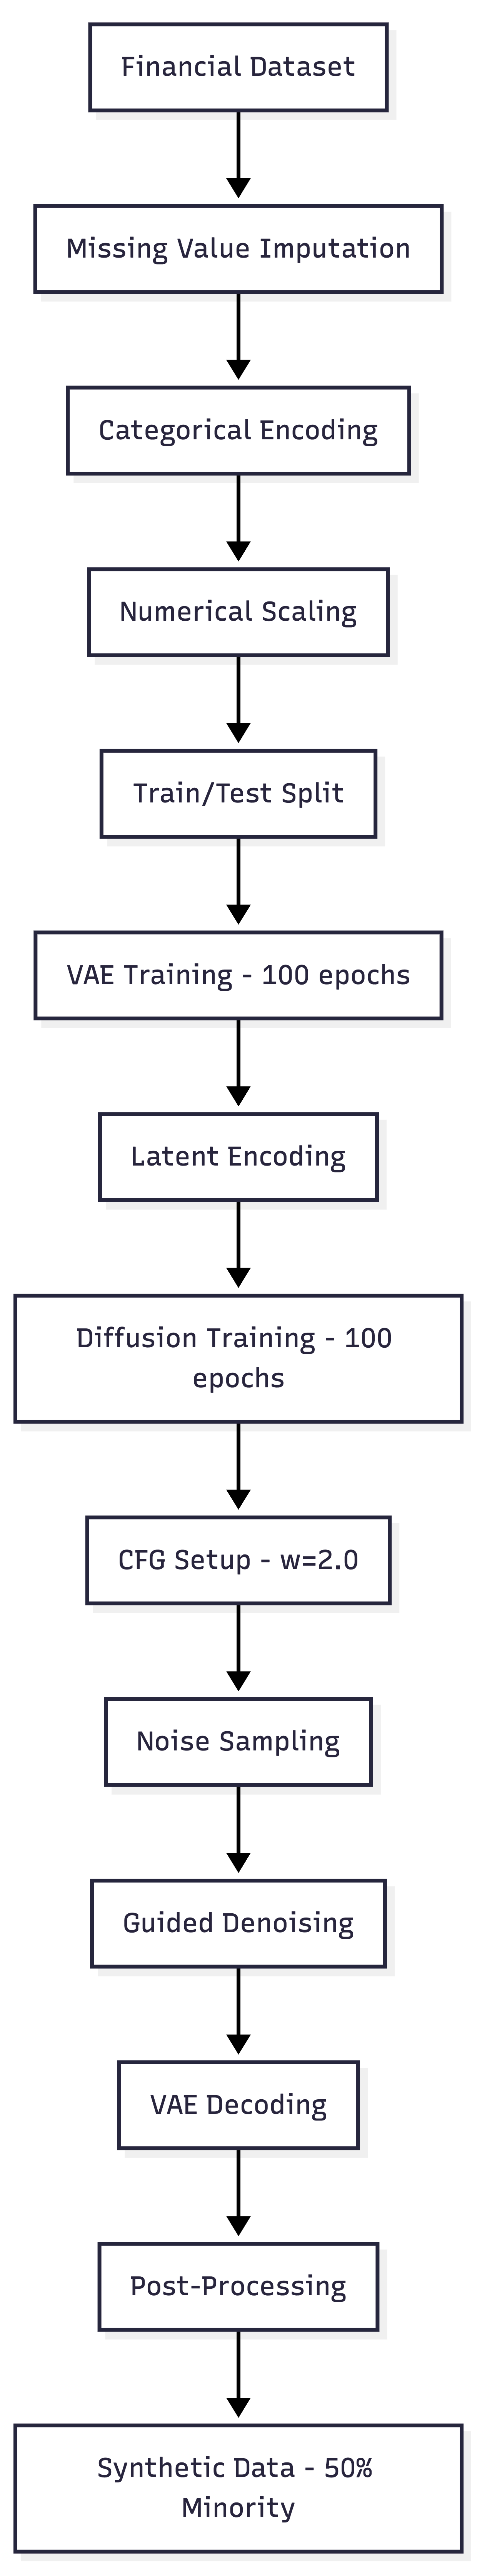
\includegraphics[width=0.45\textwidth]{img/pipeline_detailed.png}
\caption{RE-TabSyn step-by-step pipeline: from raw financial data to balanced synthetic output with 50\% minority.}
\label{fig:pipeline_detailed}
\end{figure}

Each module is independent, receiving a well-defined input and producing a well-defined output. This modularity allows fidelity issues to be traced to a specific stage rather than the system as a whole.

The pipeline consists of five integrated modules:
\begin{enumerate}
    \item \textbf{Data Ingestion Module:} Provides unified access to all six benchmark datasets with automatic download, caching, and versioning. Each dataset is loaded through a standardized interface that identifies numerical columns, categorical columns, and the target variable. This standardization is important: without it, each dataset would require separate ad-hoc preprocessing code, making it impossible to compare results fairly across datasets.

    \item \textbf{Preprocessing Module:} Transforms raw data into model-ready tensors through a sequence of imputation, encoding, and scaling operations (detailed in Section~\ref{sec:preprocessing}). All preprocessing transformers are fit on the training split only and applied to both training and test splits, preventing any information from the test set from influencing the preprocessing parameters.

    \item \textbf{Model Training Pipeline:} Implements the two-phase training protocol: first training the VAE encoder-decoder to convergence, then training the Latent Diffusion Model with Classifier-Free Guidance on frozen VAE latent representations. Freezing the VAE during diffusion training is a deliberate choice: it ensures that the latent space geometry does not shift during diffusion training, which would invalidate the already-learned encoder and require expensive retraining.

    \item \textbf{Generation Module:} Performs latent sampling, CFG-guided denoising, VAE decoding, and reverse transformation to produce synthetic tabular data in the original feature space. The output is a Pandas DataFrame in the same format as the original data, ready for downstream use without any additional processing.

    \item \textbf{Evaluation Module:} Computes a full suite of statistical fidelity, machine learning utility, and privacy metrics, generating both numerical results and visualizations. All metrics are computed three times (once per random seed) and reported as mean and standard deviation.
\end{enumerate}

\begin{figure}[!ht]
\centering
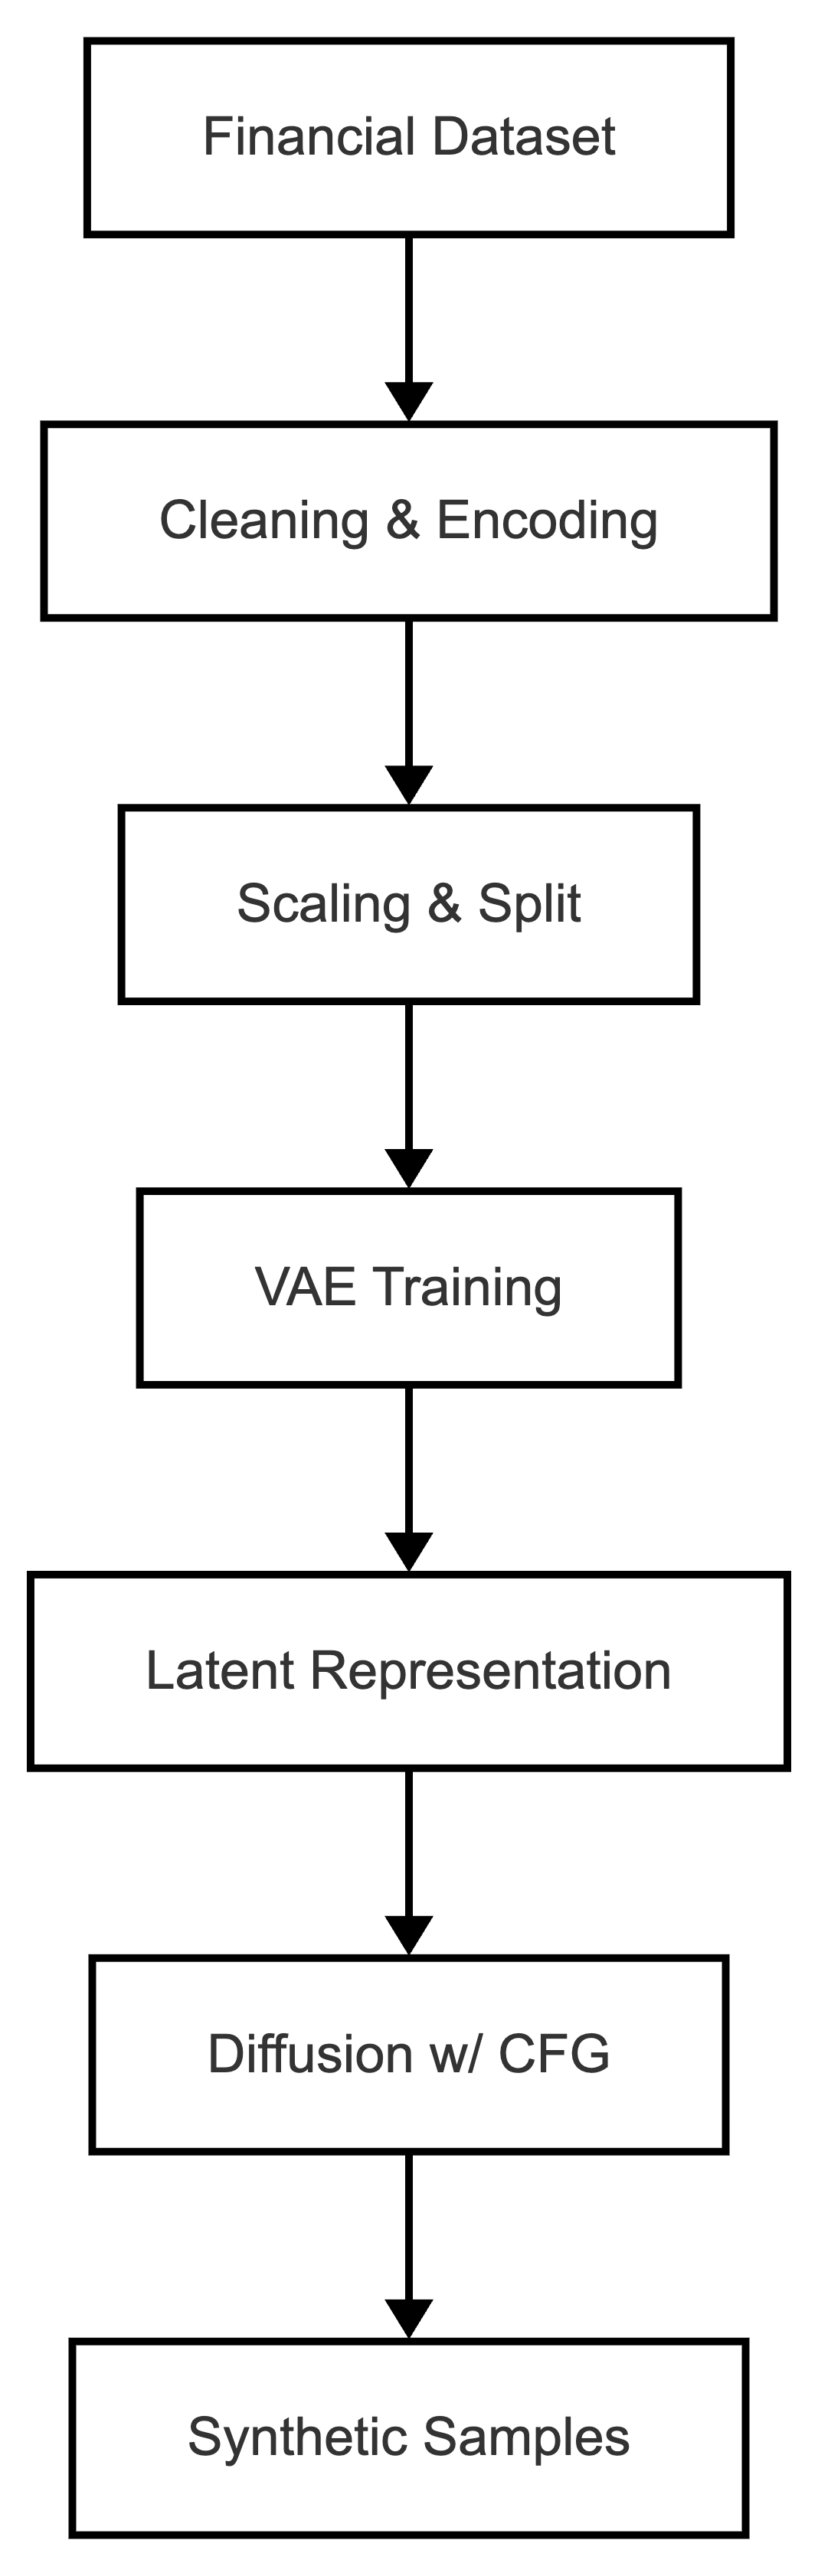
\includegraphics[width=0.4\textwidth]{img/pipeline.png}
\caption{High-level RE-TabSyn pipeline: preprocess, train VAE, train diffusion with CFG, generate synthetic data.}
\label{fig:pipeline}
\end{figure}

\section{Data Preprocessing}
\label{sec:preprocessing}

Preprocessing is where many tabular synthesis attempts fail. A model cannot recover structure that preprocessing has distorted, regardless of architectural complexity.

The preprocessing pipeline for RE-TabSyn follows four steps applied in order: (1) missing value imputation, (2) feature encoding, (3) feature scaling, and (4) train-test splitting. Each step is fit on training data only. Figure~\ref{fig:preprocessing_flow} shows the full flow from raw CSV to the final train/test splits.

\begin{figure}[!ht]
\centering
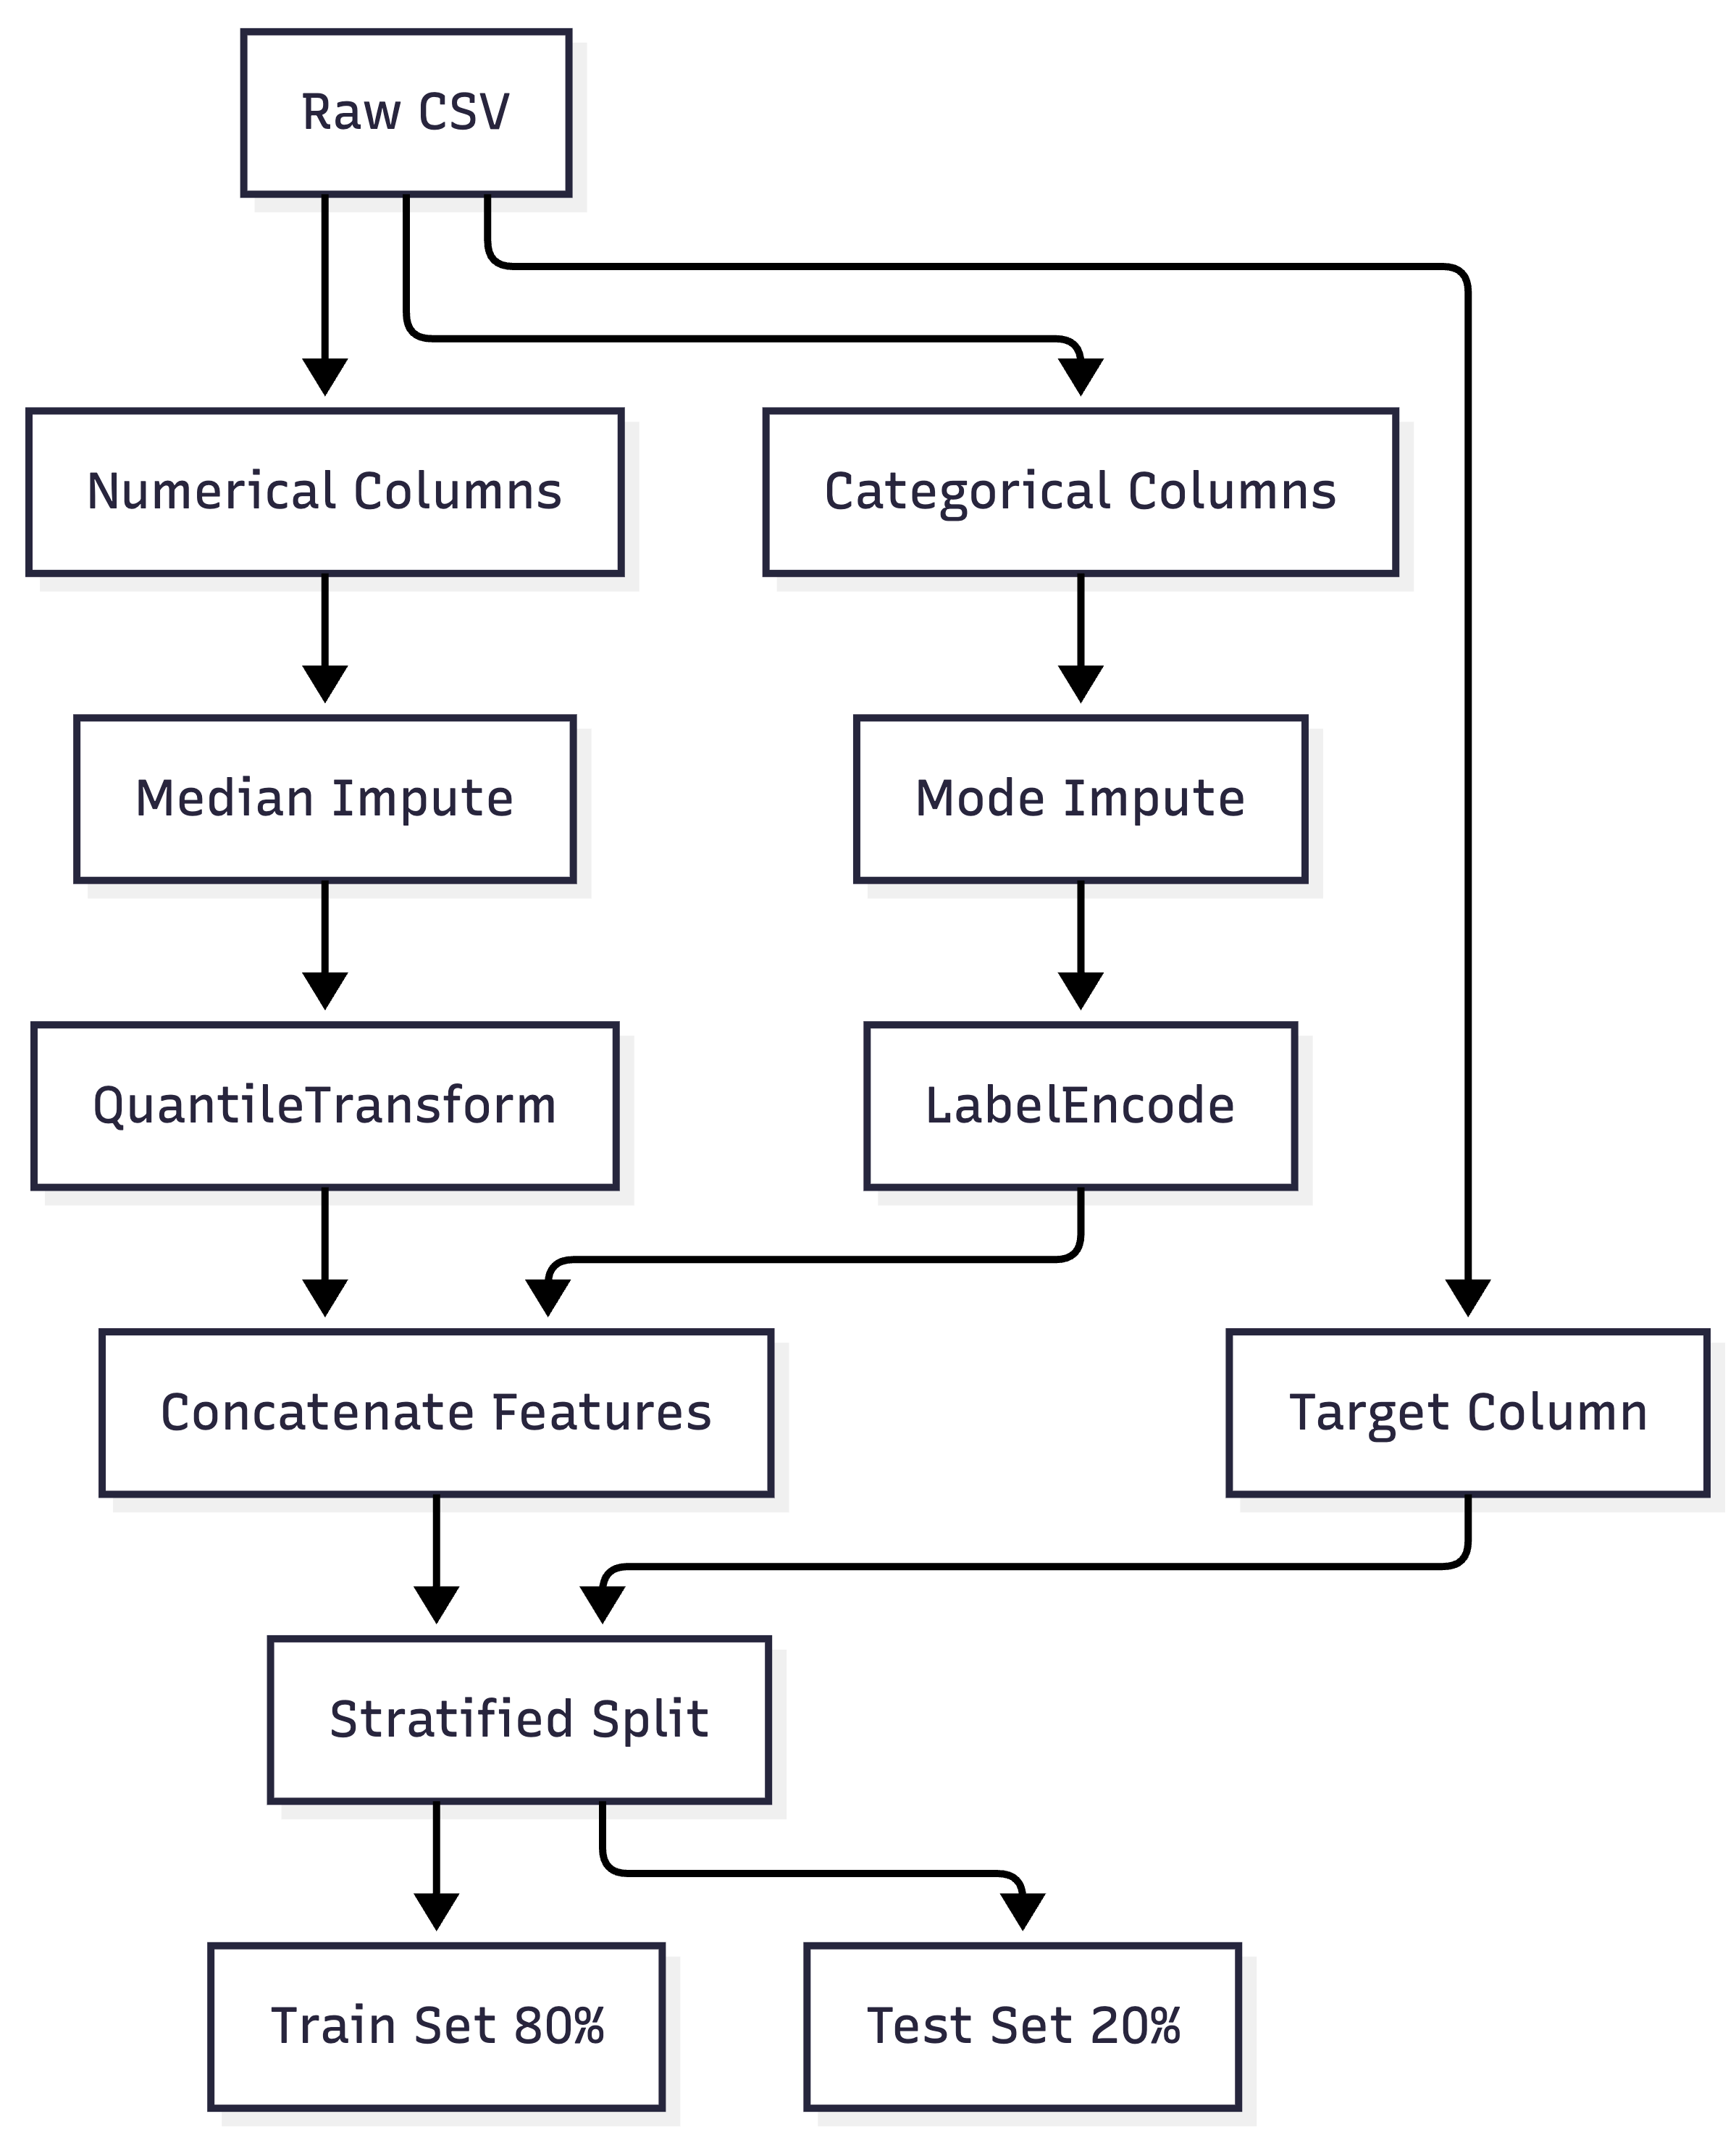
\includegraphics[width=0.55\textwidth]{img/preprocessing_flow.png}
\caption{Preprocessing flow: separate numerical (median impute, QuantileTransform) and categorical (mode impute, label encode) branches, merged then split 80/20 by stratified sampling.}
\label{fig:preprocessing_flow}
\end{figure}

\subsection{Missing value handling}

Missing values are handled through a two-strategy approach, with the choice depending on the feature type:

\textbf{Numerical columns} have missing values imputed with the column median. The median is preferred over the mean for financial data because financial distributions are often heavily skewed: a small number of very high incomes or very large transactions can pull the mean far from where most of the data lies. The median, defined as the 50th percentile, is resistant to these outliers and provides a more representative central value. For example, if a household income column has values ranging from \$20K to \$5M, the mean might be \$80K (inflated by a few ultra-high earners) while the median is \$52K (reflecting where the bulk of the population actually sits). Imputing with \$52K is more likely to produce realistic-looking records than imputing with \$80K.

\textbf{Categorical columns} have missing values imputed with the column mode (the most frequently occurring category). The rationale is that the mode represents the typical case for that column: if 60\% of applicants list ``employed'' as their employment status and the field is missing, ``employed'' is the most plausible fill. An alternative approach, treating missingness as a distinct category (for instance, ``employment\_status\_unknown''), is also supported and can be useful when the pattern of missingness itself carries information (e.g., fields that are left blank on loan applications may correlate with certain applicant behaviors).

\subsection{Feature encoding and scaling}

\textbf{Numerical Features} are transformed using a Quantile Transformer that maps arbitrary distributions to a standard normal distribution ($\mathcal{N}(0, 1)$). This step addresses a persistent problem with financial data: it is almost never normally distributed.

Consider transaction amounts. Most transactions are for small amounts (groceries, utility bills), while a few are for very large amounts (car purchases, property transactions). The resulting distribution has an extremely long right tail. If we feed this raw distribution into a VAE, the model will spend most of its capacity modelling the common small-transaction case and will poorly represent the rare large-transaction case, which is precisely where fraud and risk events are more likely to occur.

The Quantile Transformer solves this by mapping the entire distribution uniformly onto the $[0, 1]$ interval (quantile normalization) and then applying the inverse normal CDF to produce a standard normal distribution. This transformation is guaranteed to be invertible: given a transformed value, you can exactly recover the original value by applying the inverse transform. The result is that every part of the distribution is given equal representational weight during model training, regardless of how rare or common that region is in the raw data. The Gaussian output also satisfies the VAE's implicit assumption that the input space is roughly continuous and smooth.

\textbf{Categorical Features} are converted using Label Encoding, which maps each category to an integer in $\{0, 1, \ldots, K-1\}$ where $K$ is the number of distinct categories. This might seem surprising: why not use one-hot encoding, which is more common in machine learning?

The answer comes directly from the failure of TabDDPM described in the previous chapter. One-hot encoding of a categorical feature with $K$ categories creates a $K$-dimensional sparse binary vector where exactly one element is 1. When many such features are concatenated, the resulting input vector is very high-dimensional and extremely sparse. For a dataset with 10 categorical features each having 10 categories, one-hot encoding produces a 100-dimensional sparse vector (versus 10 dimensions for label encoding). This high dimensionality causes diffusion models to struggle because the noise added during the forward process creates vectors that are not sparse in the way one-hot vectors are, making the reverse denoising task poorly-conditioned.

Label encoding avoids this explosion in dimensionality. The VAE encoder then learns to embed these integer-encoded categories into continuous latent representations, effectively creating its own learned embeddings for each category. The VAE's encoder is flexible enough to learn whatever embedding is most useful for reconstruction, rather than being constrained to the fixed geometry of one-hot vectors.

\subsection{Benchmark datasets}

Table~\ref{tab:datasets} summarizes the six financial benchmark datasets used in our experiments. Each dataset was selected to represent a distinct sub-domain of financial machine learning, to cover a range of class imbalance severities, and to test the method on both small and large sample sizes.

\begin{table}[!ht]
\centering
\caption{Benchmark Dataset Characteristics}
\label{tab:datasets}
\small
\begin{tabularx}{\textwidth}{|l|c|c|c|c|X|}
\hline
\textbf{Dataset} & \textbf{Samples} & \textbf{Num.} & \textbf{Cat.} & \textbf{Min. \%} & \textbf{Domain} \\
\hline
Adult Income & 45,222 & 6 & 8 & 24.8\% & Income prediction \\
\hline
German Credit & 1,000 & 7 & 13 & 30.0\% & Credit risk \\
\hline
Bank Marketing & 41,188 & 10 & 10 & 11.3\% & Marketing response \\
\hline
Credit Approval & 690 & 6 & 9 & 44.5\% & Credit scoring \\
\hline
Lending Club & 10,000 & 8 & 4 & 20.0\% & Loan default \\
\hline
Polish Bankruptcy & 5,000 & 64 & 0 & 4.8\% & Corporate bankruptcy \\
\hline
\end{tabularx}
\end{table}

Table~\ref{tab:dataset_sources} provides the source, URL, and authenticity information for each dataset.

\begin{table}[!ht]
\centering
\caption{Dataset Sources, Repositories, and Provenance}
\label{tab:dataset_sources}
\small
\begin{tabularx}{\textwidth}{|l|l|>{\footnotesize\raggedright\arraybackslash}X|>{\raggedright\arraybackslash}X|}
\hline
\textbf{Dataset} & \textbf{Repository} & \textbf{URL} & \textbf{Original Source / Creators} \\
\hline
Adult Income & UCI ML Repository & \url{https://archive.ics.uci.edu/dataset/2/adult} & Kohavi \& Becker (1996), U.S. Census Bureau \\
\hline
German Credit & UCI ML Repository & \url{https://archive.ics.uci.edu/dataset/144/statlog+german+credit+data} & Prof.\ H. Hofmann, Universit\"{a}t Hamburg (1994) \\
\hline
Bank Marketing & UCI ML Repository & \url{https://archive.ics.uci.edu/dataset/222/bank+marketing} & Moro, Cortez \& Rita (2014), Portuguese bank records \\
\hline
Credit Approval & UCI ML Repository & \url{https://archive.ics.uci.edu/dataset/27/credit+approval} & J.R.\ Quinlan (1987), anonymised for privacy \\
\hline
Lending Club & Kaggle / LendingClub Corp. & \url{https://www.kaggle.com/datasets/wordsforthewise/lending-club} & LendingClub Corporation (SEC-regulated, publicly traded) \\
\hline
Polish Bankruptcy & UCI ML Repository & \url{https://archive.ics.uci.edu/dataset/365/polish+companies+bankruptcy+data} & Zieba et al.\ (2016), EMIS financial database \\
\hline
\end{tabularx}
\end{table}

All UCI datasets are hosted by the University of California, Irvine, the most widely used public repository for machine learning benchmarks with over 650 curated datasets and peer-reviewed provenance documentation. The Lending Club dataset originates from LendingClub Corporation, a publicly traded US fintech lender (NYSE: LC) subject to SEC and FDIC disclosure requirements; the loan data is drawn from their publicly released statistical filings. All six datasets have been used in multiple peer-reviewed publications, confirming their acceptance as valid benchmarks within the research community.

Figure~\ref{fig:dataset_overview} (Chapter~1) groups the six datasets by their degree of class imbalance, illustrating the range the benchmark covers.

A description of each dataset and the specific reason it was included:

\textbf{Adult Income} \cite{uci_adult} \textbf{(UCI Machine Learning Repository):}
Contains US Census data on 45,222 individuals with features including age, education level, occupation, and weekly working hours. The binary label indicates whether annual income exceeds \$50{,}000. Collected by Ron Kohavi and Barry Becker from the 1994 US Census database.

\textit{Selection rationale:} This is the single largest dataset in the benchmark. At 45,222 samples with a 24.8\% minority ratio, it tests whether RE-TabSyn scales to real-world dataset sizes without performance degradation. The mix of 6 numerical and 8 categorical features represents the kind of heterogeneity common in retail banking customer data. Its presence in the benchmark since 1996 and citation in thousands of studies means results on this dataset can be directly compared with a large body of prior work.

\textbf{German Credit} \cite{uci_german} \textbf{(UCI Machine Learning Repository):}
A credit risk dataset of 1,000 loan applicants from a German bank, classified as good or bad credit risks. Created by Prof.\ Hans Hofmann at Universit\"{a}t Hamburg in 1994. With 13 categorical and only 7 numerical features, it has the highest proportion of categorical attributes in the benchmark.

\textit{Selection rationale:} German Credit tests the most demanding scenario for mixed-type encoding: more categorical features than numerical ones. If the VAE cannot handle predominantly categorical data, this dataset will expose it. At 1,000 records it also represents the data-scarce setting common in niche credit risk domains, where collecting labeled default data over years of observation is expensive and slow. Prior tabular synthesis papers almost universally report results on this dataset, making it a required comparison point.

\textbf{Bank Marketing} \cite{uci_bankmarketing} \textbf{(UCI Machine Learning Repository):}
Records 41,188 direct marketing calls by a Portuguese bank between 2008 and 2013. The binary target indicates whether the contacted client subscribed to a term deposit. Assembled by Moro, Cortez, and Rita for their 2014 study on data-driven marketing prediction.

\textit{Selection rationale:} Marketing conversion datasets have an imbalance structure (11.3\% subscription rate) that is lower than German Credit but higher than Polish Bankruptcy, placing it in the moderate-imbalance band where CFG guidance should provide the clearest improvement. The large dataset size (41,188 rows) pairs with German Credit to test whether results are consistent across small and large datasets. The temporal nature of the data (calls over 5 years) also introduces realistic distribution drift within the dataset, testing robustness.

\textbf{Credit Approval} \cite{uci_creditapproval} \textbf{(UCI Machine Learning Repository):}
The smallest dataset in the benchmark with only 690 records. Features and many values have been anonymised by the original contributor, J.R.\ Quinlan, to protect proprietary credit bureau information. The 44.5\% minority ratio makes it nearly balanced.

\textit{Selection rationale:} Its near-balanced class distribution makes it a stress test in the opposite direction. CFG is designed to boost minority representation, but it must not over-correct and distort an already-balanced dataset. Including Credit Approval checks that RE-TabSyn degrades gracefully when minority boosting is not needed. Its 690 records also represent the smallest realistic training set size for a generative model, testing the lower bound of data requirements.

\textbf{Lending Club Loan Data} \cite{kaggle_lendingclub} \textbf{(Kaggle / LendingClub Corporation):}
Contains application attributes and repayment outcomes for loans issued by LendingClub Corporation, a SEC-registered peer-to-peer lender. The full dataset covers millions of loans; we use a stratified subsample of 10,000 records. Features include debt-to-income ratio, loan grade, employment length, and annual income. The binary label is loan default (minority, 20\%).

\textit{Selection rationale:} This dataset is the only one in the benchmark sourced from a publicly traded company with regulatory disclosure obligations, giving it the strongest real-world provenance of the six. The features (debt-to-income ratio, loan grade, employment length) are the exact variables used in actual underwriting decisions, making performance on this dataset directly relevant to production deployment. The 20\% default rate represents a realistic operational imbalance for consumer lending.

\textbf{Polish Bankruptcy} \cite{uci_polishbankruptcy} \textbf{(UCI Machine Learning Repository):}
Financial ratio data for Polish companies collected from the Emerging Markets Information Service, i.e., EMIS, database, covering the years 2000--2012. Compiled by Zieba et al.\ for their 2016 bankruptcy prediction study. Contains 64 purely numerical financial ratios (current ratio, debt-to-equity, return on assets, and similar) with a 4.8\% bankruptcy rate.

\textit{Selection rationale:} Polish Bankruptcy is the hardest dataset in the benchmark on two dimensions simultaneously. First, the 4.8\% minority ratio is the most extreme imbalance, where class-conditional generation must work hardest. Second, the 64-dimensional purely numerical feature space is the largest in the benchmark, testing whether the 64-dimensional VAE latent space is sufficient to encode all relevant structure. This dataset is where RE-TabSyn's CFG mechanism produces its most visible effect, boosting minority representation from 4.8\% to 47.8\%.

These datasets were selected to cover a wide range of:
\begin{enumerate}
    \item \textbf{Sample sizes:} From 690 (Credit Approval) to 45,222 (Adult Income), testing scalability across two orders of magnitude.
    \item \textbf{Feature compositions:} From purely numerical (Polish Bankruptcy, 64 features) to highly mixed-type (German Credit, 13 categorical and 7 numerical features), testing the mixed-type encoding capability.
    \item \textbf{Imbalance severities:} From near-balanced (Credit Approval at 44.5\%) to extreme imbalance (Polish Bankruptcy at 4.8\%), testing the limits of minority boosting.
    \item \textbf{Financial sub-domains:} Income prediction, credit risk, marketing response, loan performance, and corporate bankruptcy.
\end{enumerate}

\section{Model Configurations}

This section details the architectural configurations and hyperparameters for RE-TabSyn and all baseline methods. All models were configured following their respective authors' recommendations, with adjustments for the financial tabular data domain where necessary.

Table~\ref{tab:hyperparams} provides a consolidated reference of all RE-TabSyn hyperparameters. The rationale for each choice is explained in the subsections that follow.

\begin{table}[!ht]
\centering
\caption{Complete RE-TabSyn Hyperparameter Reference}
\label{tab:hyperparams}
\small
\begin{tabularx}{\textwidth}{|l|l|X|}
\hline
\textbf{Component} & \textbf{Hyperparameter} & \textbf{Value} \\
\hline
\multirow{5}{*}{VAE} & Encoder hidden dims & [256, 128] \\
                     & Decoder hidden dims & [128, 256] \\
                     & Latent dimension $d$ & 64 \\
                     & Activation & ReLU \\
                     & KL weight $\beta$ & 0.1 \\
\hline
\multirow{6}{*}{Diffusion (DiT)} & Number of layers & 4 \\
                                  & Hidden dimension & 256 \\
                                  & Attention heads & 4 \\
                                  & Head dimension & 64 \\
                                  & Timesteps $T$ & 1000 \\
                                  & Noise schedule & Linear \\
                                  & $\beta_1$ (start) & $10^{-4}$ \\
                                  & $\beta_T$ (end) & 0.02 \\
\hline
\multirow{4}{*}{Embeddings} & Time embed dim & 128 \\
                             & Time projection dim & 256 \\
                             & Class vocab size & 3 (0, 1, $\emptyset$) \\
                             & Class embed dim & 256 \\
\hline
\multirow{2}{*}{CFG} & Label dropout $p_{uncond}$ & 0.10 \\
                      & Guidance scale $w$ & 2.0 \\
\hline
\multirow{4}{*}{Training} & Optimiser & Adam \\
                           & Learning rate & $10^{-3}$ \\
                           & Batch size & 256 \\
                           & Epochs per phase & 100 \\
\hline
\multirow{2}{*}{Evaluation} & Train/test split & 80\% / 20\% \\
                              & Random seeds & 42, 123, 456 \\
\hline
\end{tabularx}
\end{table}

\subsection{RE-TabSyn architecture}

The full RE-TabSyn architecture is configured as follows:

\textbf{VAE Encoder:} A Multi-Layer Perceptron, i.e., MLP, with hidden dimensions [256, 128] and ReLU activations. ReLU, i.e., Rectified Linear Unit, was chosen over alternatives like GELU or Tanh because it is computationally cheap, avoids saturation in the middle layers, and provides sufficient non-linearity for the encoding task. The two hidden layers compress the data progressively from the input dimension down to 64. The encoder produces both a mean vector $\mu \in \mathbb{R}^{64}$ and a log-variance vector $\log \sigma^2 \in \mathbb{R}^{64}$ for the 64-dimensional latent space.

\textbf{VAE Decoder:} A mirror architecture [128, 256] with separate output heads. The mirror structure is not strictly required but is a common and effective design: the decoder should roughly invert the encoder, and matching the hidden dimensions provides a natural correspondence. The separate output heads are the distinguishing design choice: a linear projection (followed by the inverse quantile transform) for numerical features, and a softmax projection (followed by argmax) for categorical features. This means each categorical column gets its own softmax head with dimensionality equal to the number of categories in that column, ensuring the decoder can produce a valid probability distribution over all possible values.

\textbf{Diffusion Backbone (DiT):} A Diffusion Transformer architecture with 4 layers, hidden dimension 256, and 4 attention heads (64 dimensions per head). The noise schedule uses $T = 1000$ timesteps with linear $\beta$ variance schedule from $\beta_1 = 10^{-4}$ to $\beta_T = 0.02$. These are the default settings from the original DDPM paper \cite{ho2020ddpm} and have produced consistent results across many subsequent applications.

\textbf{Guidance Parameters:} Label dropout rate $p_{uncond} = 0.10$ during training, meaning 10\% of training samples have their class label replaced with the null token $\emptyset$. Guidance scale $w = 2.0$ during inference, producing near-50\% minority ratios in practice.

\textbf{Embeddings:} Sinusoidal time embeddings with 128-dimensional projection. The sinusoidal embedding maps an integer timestep $t \in \{1, ..., 1000\}$ to a 64-dimensional vector using sine and cosine functions of different frequencies, following Vaswani et al.\ \cite{vaswani2017attention}. These are then projected through a two-layer MLP to a 256-dimensional representation matching the DiT's hidden dimension. Learned class embeddings for 3 tokens (class 0, class 1, null $\emptyset$) are initialized randomly and optimized during training. The null token is treated as a third class, allowing the model to learn a distinct representation for the unconditional case.

\subsection{Baseline configurations}

RE-TabSyn is compared against four established methods. All baseline implementations use their official codebases to ensure fair comparison:

\textbf{CTGAN:} Mode-specific normalization (with variational Gaussian mixture models), a PAC (Packing) discriminator that looks at a pack of 10 samples simultaneously to reduce mode collapse, embedding dimension 128 for categorical features, generator and discriminator hidden dimensions both [256, 256], batch size 500, trained for 100 epochs. The PAC discriminator is a specific improvement to the standard GAN discriminator that helps detect mode collapse by comparing batches of generated samples. Implemented via the SDV (Synthetic Data Vault) library.

\textbf{TVAE:} Standard VAE with CTGAN-compatible tabular preprocessing (same mode-specific normalization), embedding dimension 128, encoder and decoder hidden dimensions both [128, 128], trained for 100 epochs with the default ELBO objective. Implemented via the SDV library.

\textbf{TabDDPM:} Gaussian diffusion for numerical features, multinomial diffusion for categorical features, MLP backbone (not Transformer) with hidden dimensions [256, 256, 256], 1,000 diffusion steps, trained for 100 epochs. The MLP backbone is the original paper's design choice; it does not include self-attention, which is one reason it cannot capture complex inter-feature dependencies as well as the DiT. Implemented from the official repository by Kotelnikov et al.\ \cite{kotelnikov2023tabddpm}.

\textbf{TabSyn:} VAE with a Transformer-based latent diffusion model, without CFG. TabSyn's VAE uses a more complex architecture than RE-TabSyn's (it processes each feature through a separate tokenizer before encoding), and its diffusion backbone is also Transformer-based. This is the highest-fidelity tabular synthesis method in the literature at the time of this work. Implemented from the official repository by Zhang et al.\ \cite{zhang2024tabsyn}.

\subsection{Method comparison at a glance}

Table~\ref{tab:method_comparison} summarises the architectural properties of all five methods side by side, showing where RE-TabSyn sits relative to the alternatives and why each architectural choice differs.

\begin{table}[!ht]
\centering
\caption{Architectural Comparison Across All Methods}
\label{tab:method_comparison}
\small
\begin{tabularx}{\textwidth}{|l|C|C|C|C|C|}
\hline
\textbf{Property} & \textbf{CTGAN} & \textbf{TVAE} & \textbf{TabDDPM} & \textbf{TabSyn} & \textbf{RE-TabSyn} \\
\hline
Framework & GAN & VAE & Diffusion & VAE + Diffusion & VAE + Diffusion + CFG \\
\hline
Generative model & Generator & Decoder & MLP diffusion & DiT diffusion & DiT diffusion \\
\hline
Latent space & No & Yes (128-d) & No & Yes (learned) & Yes (64-d Gaussian) \\
\hline
Handles mixed types & Yes (mode norm.) & Yes (mode norm.) & Poor & Yes & Yes \\
\hline
Minority class control & No & No & No & No & Yes (CFG, $w$) \\
\hline
Class conditioning & No & No & No & No & Yes \\
\hline
Training phases & 1 & 1 & 1 & 2 & 2 \\
\hline
Fast sampling possible & N/A & N/A & DDIM & DDIM & DDIM \\
\hline
Formal DP support & No & No & No & No & Planned (Opacus) \\
\hline
\end{tabularx}
\end{table}

The table confirms one structural fact: RE-TabSyn is the only method among the five that offers minority class control. Every other method generates data according to whatever class distribution exists in the training data. If fraud is 5\% of the training set, every other method will generate fraud 5\% of the time. RE-TabSyn can change this at inference time, with no retraining.

\section{Training Procedures}

Training proceeds in two distinct, sequential phases. The two-phase structure decouples the representation learning problem, i.e., VAE, from the generative modeling problem, i.e., diffusion, allowing each component to be optimized independently. Figure~\ref{fig:two_phase_training} shows the structure of both phases.

\begin{figure}[!ht]
\centering
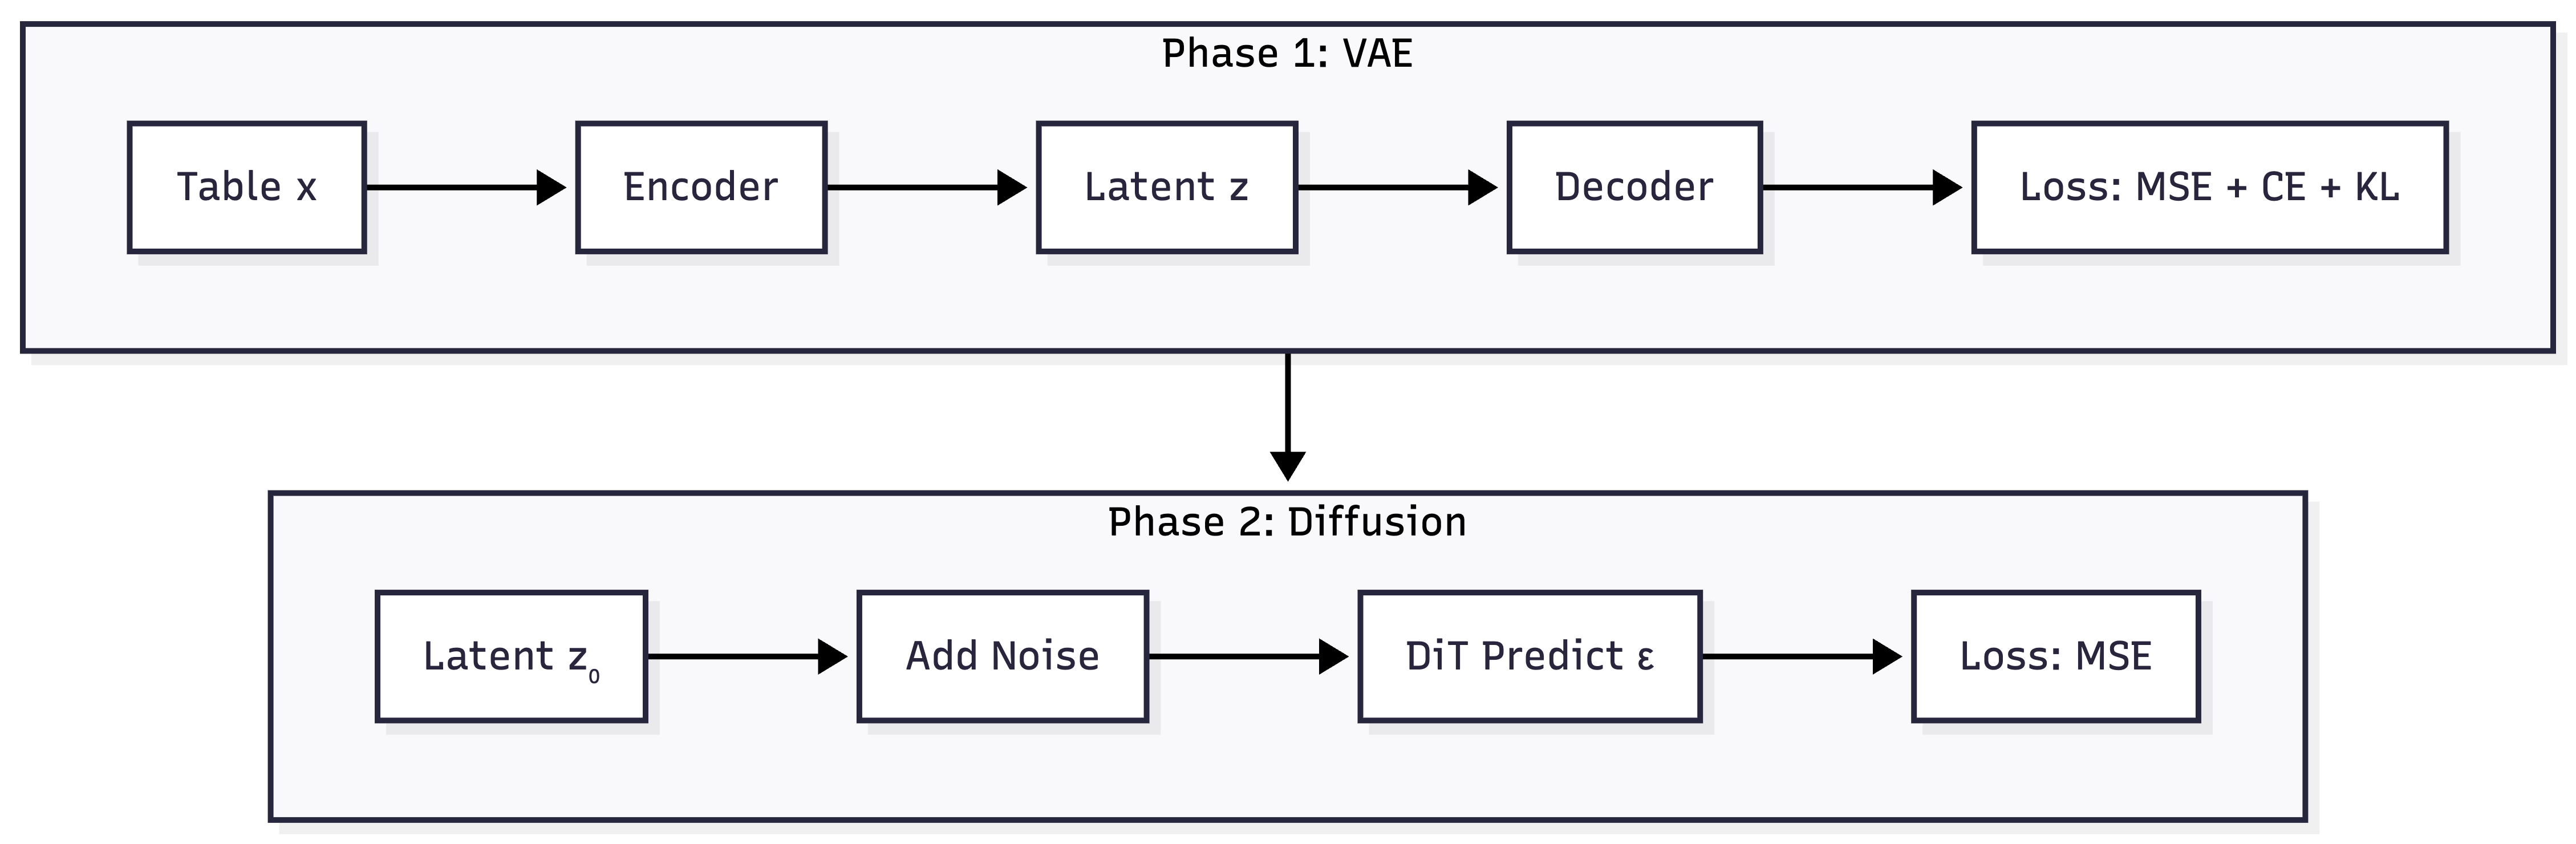
\includegraphics[width=\textwidth]{img/two_phase_training.png}
\caption{Two-phase training: Phase 1 trains the VAE (MSE + CE + KL loss); Phase 2 freezes the VAE and trains the diffusion model (MSE noise prediction).}
\label{fig:two_phase_training}
\end{figure}

\textbf{Phase 1 -- VAE Training (Epochs 1--100):}

\begin{enumerate}
    \item Raw data is preprocessed as described in Section~\ref{sec:preprocessing} and split into training (80\%) and test (20\%) sets. The 80/20 split is standard in machine learning practice. The test set is held out entirely during model training and used only for evaluation.

    \item The VAE is trained to minimize the combined loss: $\mathcal{L}_{VAE} = \mathcal{L}_{MSE} + \mathcal{L}_{CE} + 0.1 \cdot \mathcal{L}_{KL}$. The loss is computed on the training set and the weights are updated using gradient descent. No data augmentation is applied during VAE training.

    \item The KL weight $\beta = 0.1$ is fixed (not annealed). Some VAE training protocols gradually increase $\beta$ from 0 to its final value over the course of training (``KL annealing''), which can help avoid posterior collapse early in training when the reconstruction loss dominates. We found that a fixed $\beta = 0.1$ achieves stable training without collapse across all six datasets, avoiding the additional hyperparameter of the annealing schedule.

    \item Adam optimizer \cite{kingma2015adam} is used with learning rate $10^{-3}$ and default momentum parameters ($\beta_1 = 0.9$, $\beta_2 = 0.999$). Adam is the standard choice for VAE training because it adapts the learning rate per parameter, handling the different scales of numerical and categorical features gracefully. Batch size 256 provides a good balance between gradient noise (smaller batches provide noisier but more frequent updates) and computational efficiency.

    \item Training converges when reconstruction loss stabilizes, typically within 50--80 epochs. The training loop monitors the validation loss (on the held-out 20\% of training data) and saves the model checkpoint at each epoch. The final model used for latent encoding is the checkpoint with the lowest validation loss.
\end{enumerate}

\begin{figure}[!ht]
\centering
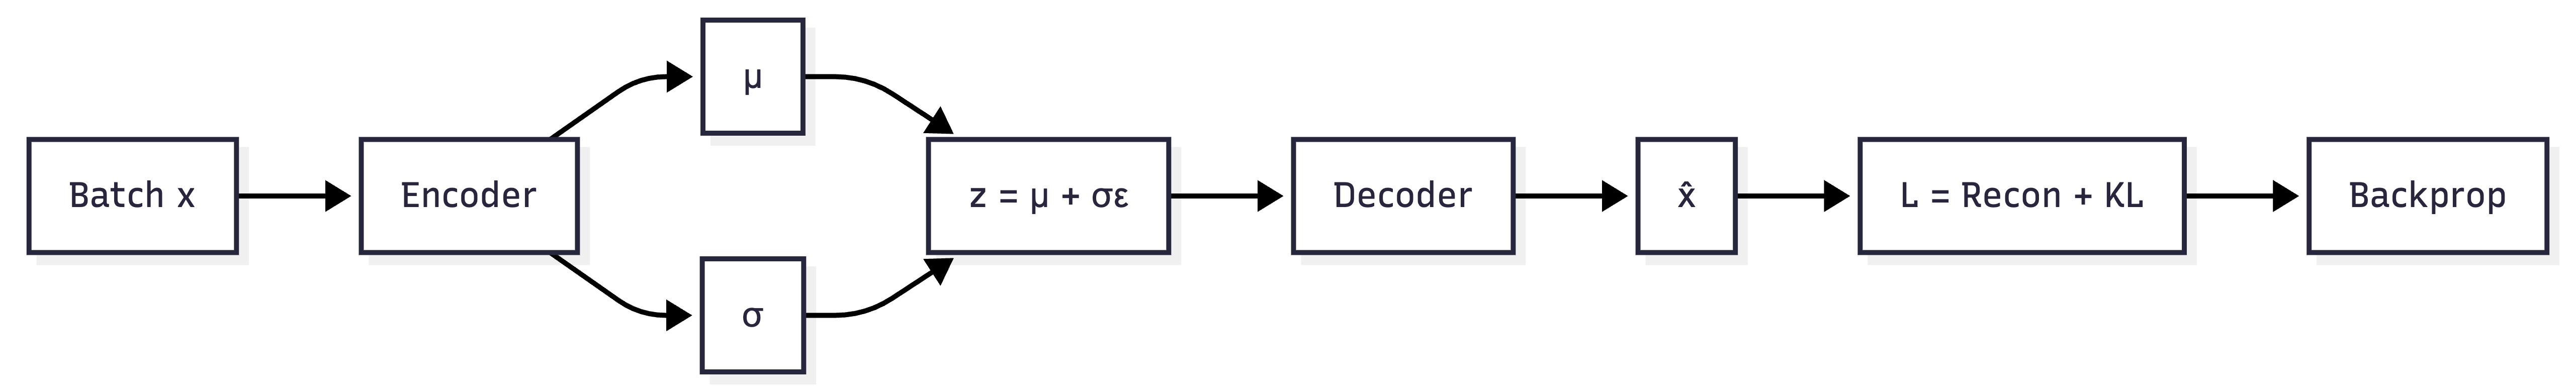
\includegraphics[width=\textwidth]{img/vae_training_loop.png}
\caption{VAE training loop: encode to $(\mu, \sigma)$, reparameterise to $\mathbf{z}$, decode to $\hat{\mathbf{x}}$, backpropagate reconstruction + KL loss.}
\label{fig:vae_training_loop}
\end{figure}

\textbf{Phase 2 -- Diffusion Training (Epochs 1--100):}

\begin{enumerate}
    \item VAE weights are frozen. Freezing is necessary: if the VAE continued training during Phase 2, the latent representations of training data would shift, invalidating the latent codes that the diffusion model has already learned to model. Freezing ensures the latent space is stable throughout Phase 2.

    \item All training data is encoded into the 64-dimensional latent space using the frozen VAE encoder. This encoding step is done once, before training begins, and the resulting latent vectors are cached. This avoids the computational cost of re-encoding the training data at every training step.

    \item For each training step, the following operations are performed: a random timestep $t \sim \mathcal{U}(1, 1000)$ is sampled uniformly; Gaussian noise $\epsilon \sim \mathcal{N}(0, I)$ is sampled; with probability $p_{uncond} = 0.10$, the class label $y$ for this sample is replaced with the null token $\emptyset$; the noisy latent $\mathbf{z}_t = \sqrt{\bar{\alpha}_t}\mathbf{z}_0 + \sqrt{1-\bar{\alpha}_t}\epsilon$ is computed; the DiT predicts $\hat{\epsilon} = \epsilon_\theta(\mathbf{z}_t, t, y)$; and the MSE loss $\|\epsilon - \hat{\epsilon}\|^2$ is backpropagated.

    \item Adam optimizer with the same learning rate $10^{-3}$ and batch size 256 as Phase 1. Using the same optimizer settings for both phases simplifies the hyperparameter search.

    \item All experiments are run with three random seeds (42, 123, 456) to assess result variance. Each seed controls the random initialization of all model weights, the random sampling of timesteps and noise during training, and the random ordering of training batches. Reporting mean and standard deviation across three seeds confirms that the findings are not artifacts of a single initialization.
\end{enumerate}

\begin{figure}[!ht]
\centering
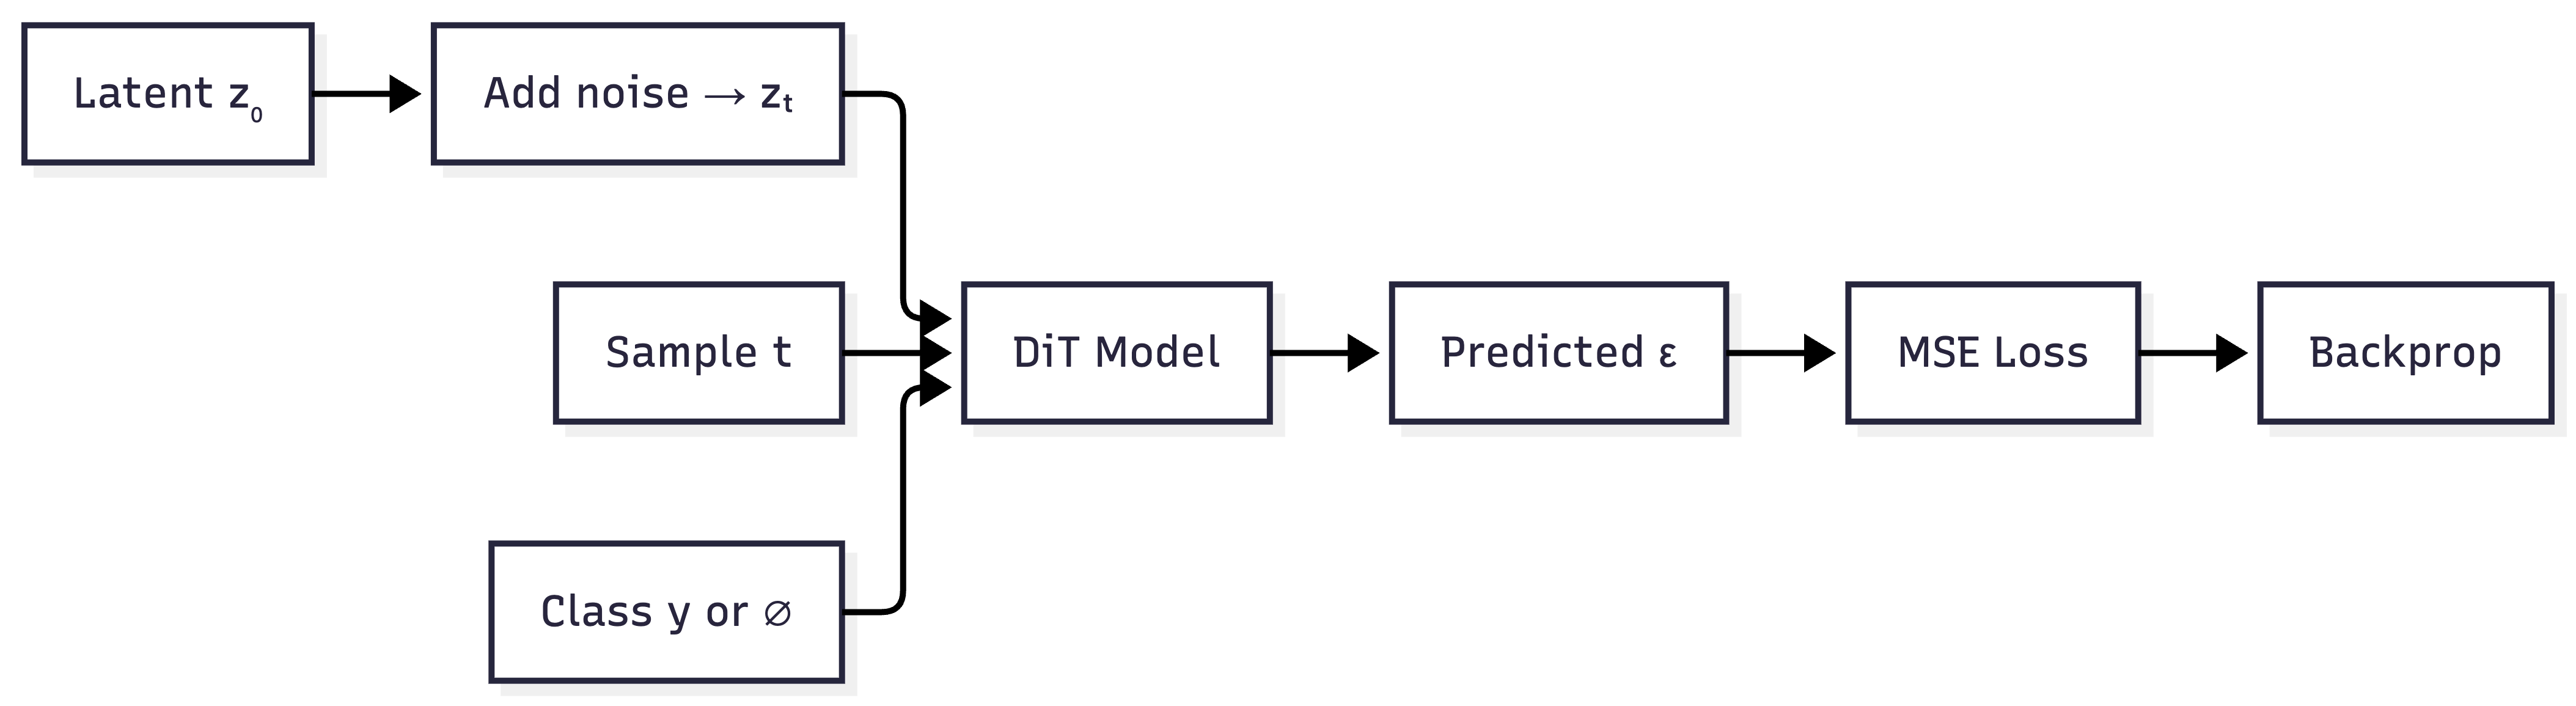
\includegraphics[width=\textwidth]{img/diffusion_training_loop.png}
\caption{Diffusion training loop: noise frozen latent $\mathbf{z}_0$, predict noise $\hat{\epsilon}$ with DiT, backpropagate MSE loss.}
\label{fig:diffusion_training_loop}
\end{figure}

\section{Synthetic Data Generation Procedure}

Generation with RE-TabSyn follows a structured four-step protocol. Once trained, the model can generate any number of synthetic samples with any desired minority ratio without retraining.

\textbf{Step 1 -- Latent Initialization:} Sample $N$ initial noise vectors from $\mathcal{N}(0, I)$ in the 64-dimensional latent space. These are pure random noise vectors, which are the starting point of the reverse diffusion process. To generate balanced data with 50\% minority representation, half of the $N$ samples are assigned class label $y = 1$ and half are assigned $y = 0$. The split can be adjusted to generate any desired ratio: to get 30\% minority, assign 30\% of samples $y = 1$ and 70\% $y = 0$.

\textbf{Step 2 -- CFG-Guided Denoising:} For each of the $T = 1000$ reverse diffusion steps (iterating from $t = T$ down to $t = 1$). Figure~\ref{fig:cfg_denoising_step} shows the two-pass structure of each step:
\begin{enumerate}
    \item Compute the conditional noise prediction: $\epsilon_{cond} = \epsilon_\theta(\mathbf{z}_t, t, y)$. This is a forward pass through the DiT with the class label.
    \item Compute the unconditional noise prediction: $\epsilon_{uncond} = \epsilon_\theta(\mathbf{z}_t, t, \emptyset)$. This is a second forward pass through the same DiT with the null token.
    \item Apply CFG: $\tilde{\epsilon} = \epsilon_{uncond} + w \cdot (\epsilon_{cond} - \epsilon_{uncond})$ with $w = 2.0$.
    \item Update the latent: $\mathbf{z}_{t-1} = f(\mathbf{z}_t, \tilde{\epsilon}, t)$ using the DDPM reverse step formula.
\end{enumerate}

\begin{figure}[!ht]
\centering
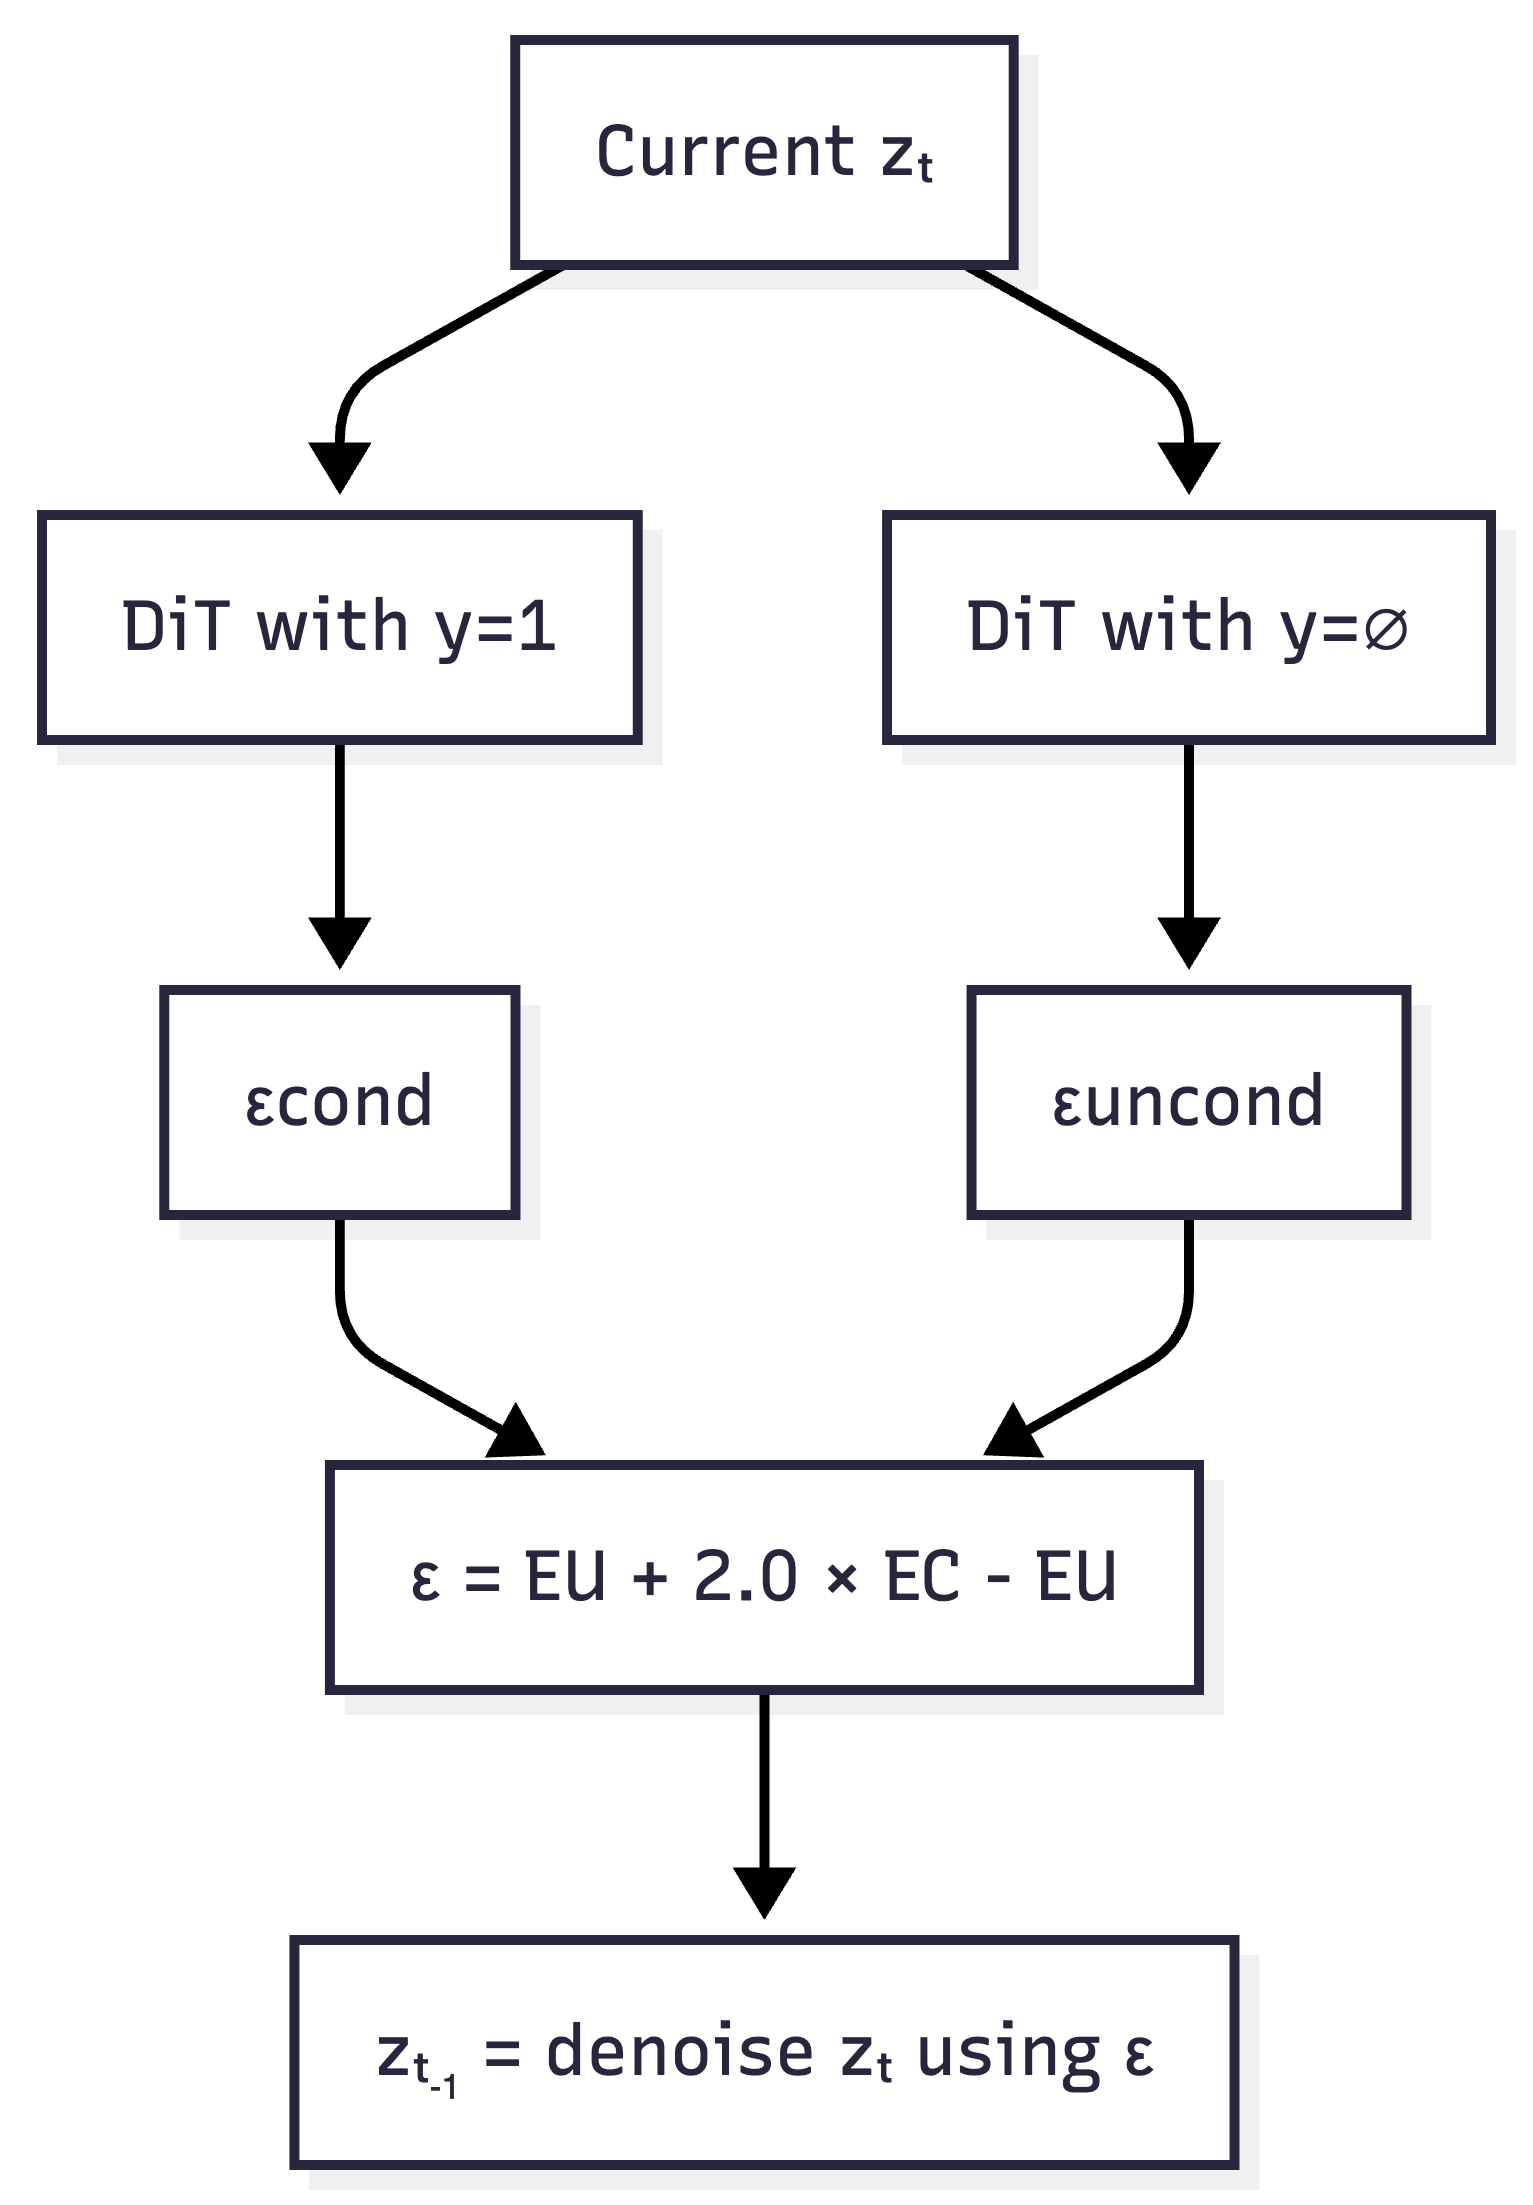
\includegraphics[width=0.80\textwidth]{img/cfg_denoising_step.png}
\caption{Single CFG denoising step: two DiT passes (conditional and unconditional) blended with $w=2.0$ to produce $\mathbf{z}_{t-1}$.}
\label{fig:cfg_denoising_step}
\end{figure}

This procedure requires two forward passes through the DiT per denoising step (one conditional, one unconditional), making CFG generation approximately twice as slow as unconditional generation. For generating 1,000 synthetic samples, this amounts to 2,000,000 DiT forward passes in total ($2 \times 1000 \text{ steps} \times 1000 \text{ samples}$). On the M3 chip, this takes roughly a few minutes per dataset, which is acceptable for research use. Production deployments could accelerate this using fast sampling schedules like DDIM \cite{ho2020ddpm}, which achieves comparable quality in as few as 50 steps.

\textbf{Step 3 -- VAE Decoding:} Pass the denoised latent vectors $\mathbf{z}_0$ (the output of Step 2 after all 1000 denoising steps) through the frozen VAE decoder to reconstruct tabular features.

Numerical features are produced directly from the decoder's linear output heads as real-valued numbers in the transformed (Gaussian) space. Categorical features are obtained via argmax over the softmax probabilities from each categorical output head: the category with the highest predicted probability is selected. This argmax step is the only non-differentiable operation in the entire pipeline, and it occurs only during generation (not during training), so it does not create any training issues.

\textbf{Step 4 -- Reverse Transformation:} Apply the inverse preprocessing pipeline to convert model outputs back to the original feature space. Numerical features are mapped from the Gaussian $\mathcal{N}(0,1)$ representation back to the original distribution via the Inverse Quantile Transformer — an exact inverse that preserves percentile rank. Categorical features are recovered by Inverse Label Encoding, mapping integers back to their original string values (e.g., 2 maps back to ``self-employed'').

The result is a Pandas DataFrame in the original feature space, matching the format of the real data exactly. It can be used directly for downstream machine learning tasks without any additional processing.

\section{Evaluation Framework}

Our evaluation follows the three-pillar framework illustrated in Figure~\ref{fig:evaluation_framework}.

\begin{figure}[!ht]
\centering
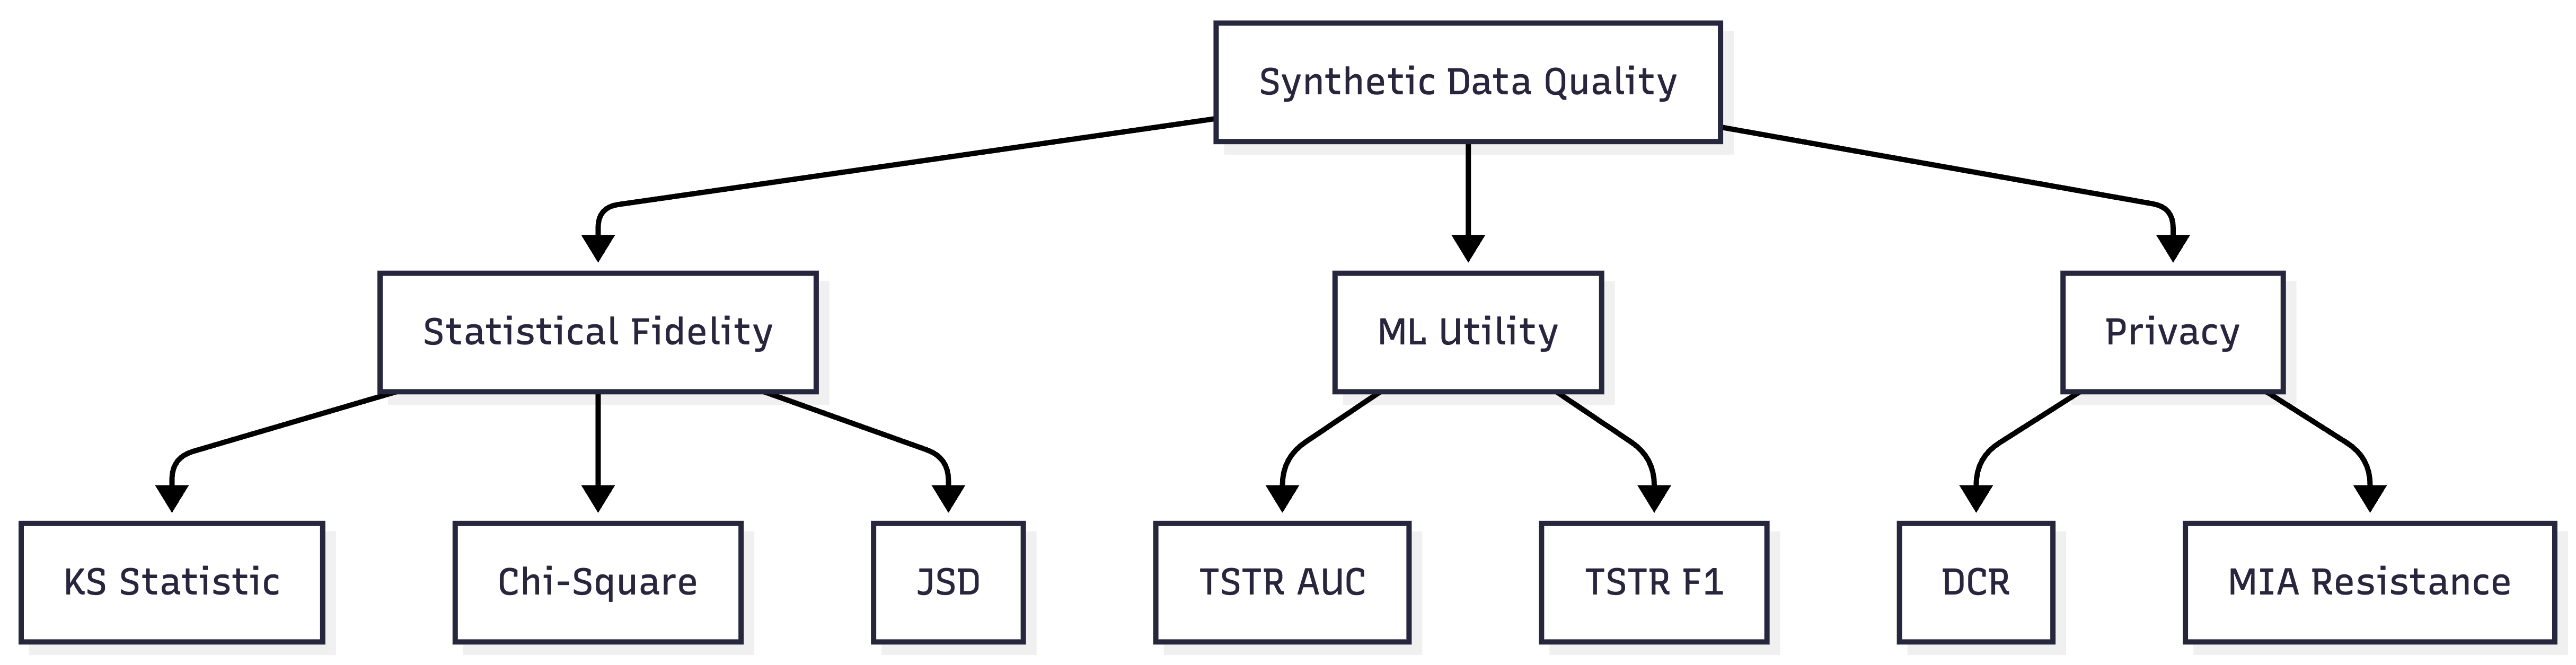
\includegraphics[width=\textwidth]{img/evaluation_framework.png}
\caption{Three-pillar evaluation framework: statistical fidelity (KS, Chi-Square, JSD), ML utility (TSTR AUC, F1), and privacy (DCR, MIA).}
\label{fig:evaluation_framework}
\end{figure}

\subsection{Pillar 1: Statistical fidelity}

Statistical fidelity measures how closely the marginal and joint distributions of synthetic data match those of real data. Two metrics are used.

\textbf{Kolmogorov-Smirnov, i.e., KS, Statistic} \cite{massey1951ks}: For each numerical column, compute the maximum absolute difference between the empirical cumulative distribution functions (CDFs) of the real and synthetic data:
\[
D_{KS} = \sup_x |F_{real}(x) - F_{synth}(x)|
\]
where $F_{real}$ and $F_{synth}$ are the empirical CDFs of the real and synthetic column values respectively. Values range from 0 (identical distributions) to 1 (completely different). We report the average KS across all numerical columns. The KS test is non-parametric: it makes no assumptions about the shape of the distribution and detects differences anywhere in the distribution, not just in the mean or variance.

\textbf{Correlation Preservation:} Compute the $d \times d$ pairwise Pearson correlation matrices for the real and synthetic data (where $d$ is the number of features). Report the mean absolute difference between corresponding entries:
\[
\text{Corr Error} = \frac{1}{d^2} \sum_{i,j} |r_{ij}^{real} - r_{ij}^{synth}|
\]
Lower values indicate better preservation of inter-feature relationships. This captures a dimension that the KS statistic misses: two synthetic datasets could have identical marginal distributions but completely different correlation structures, making them unsuitable for downstream modeling despite appearing similar column-by-column.

\subsection{Pillar 2: Machine learning utility}

\begin{figure}[!ht]
\centering
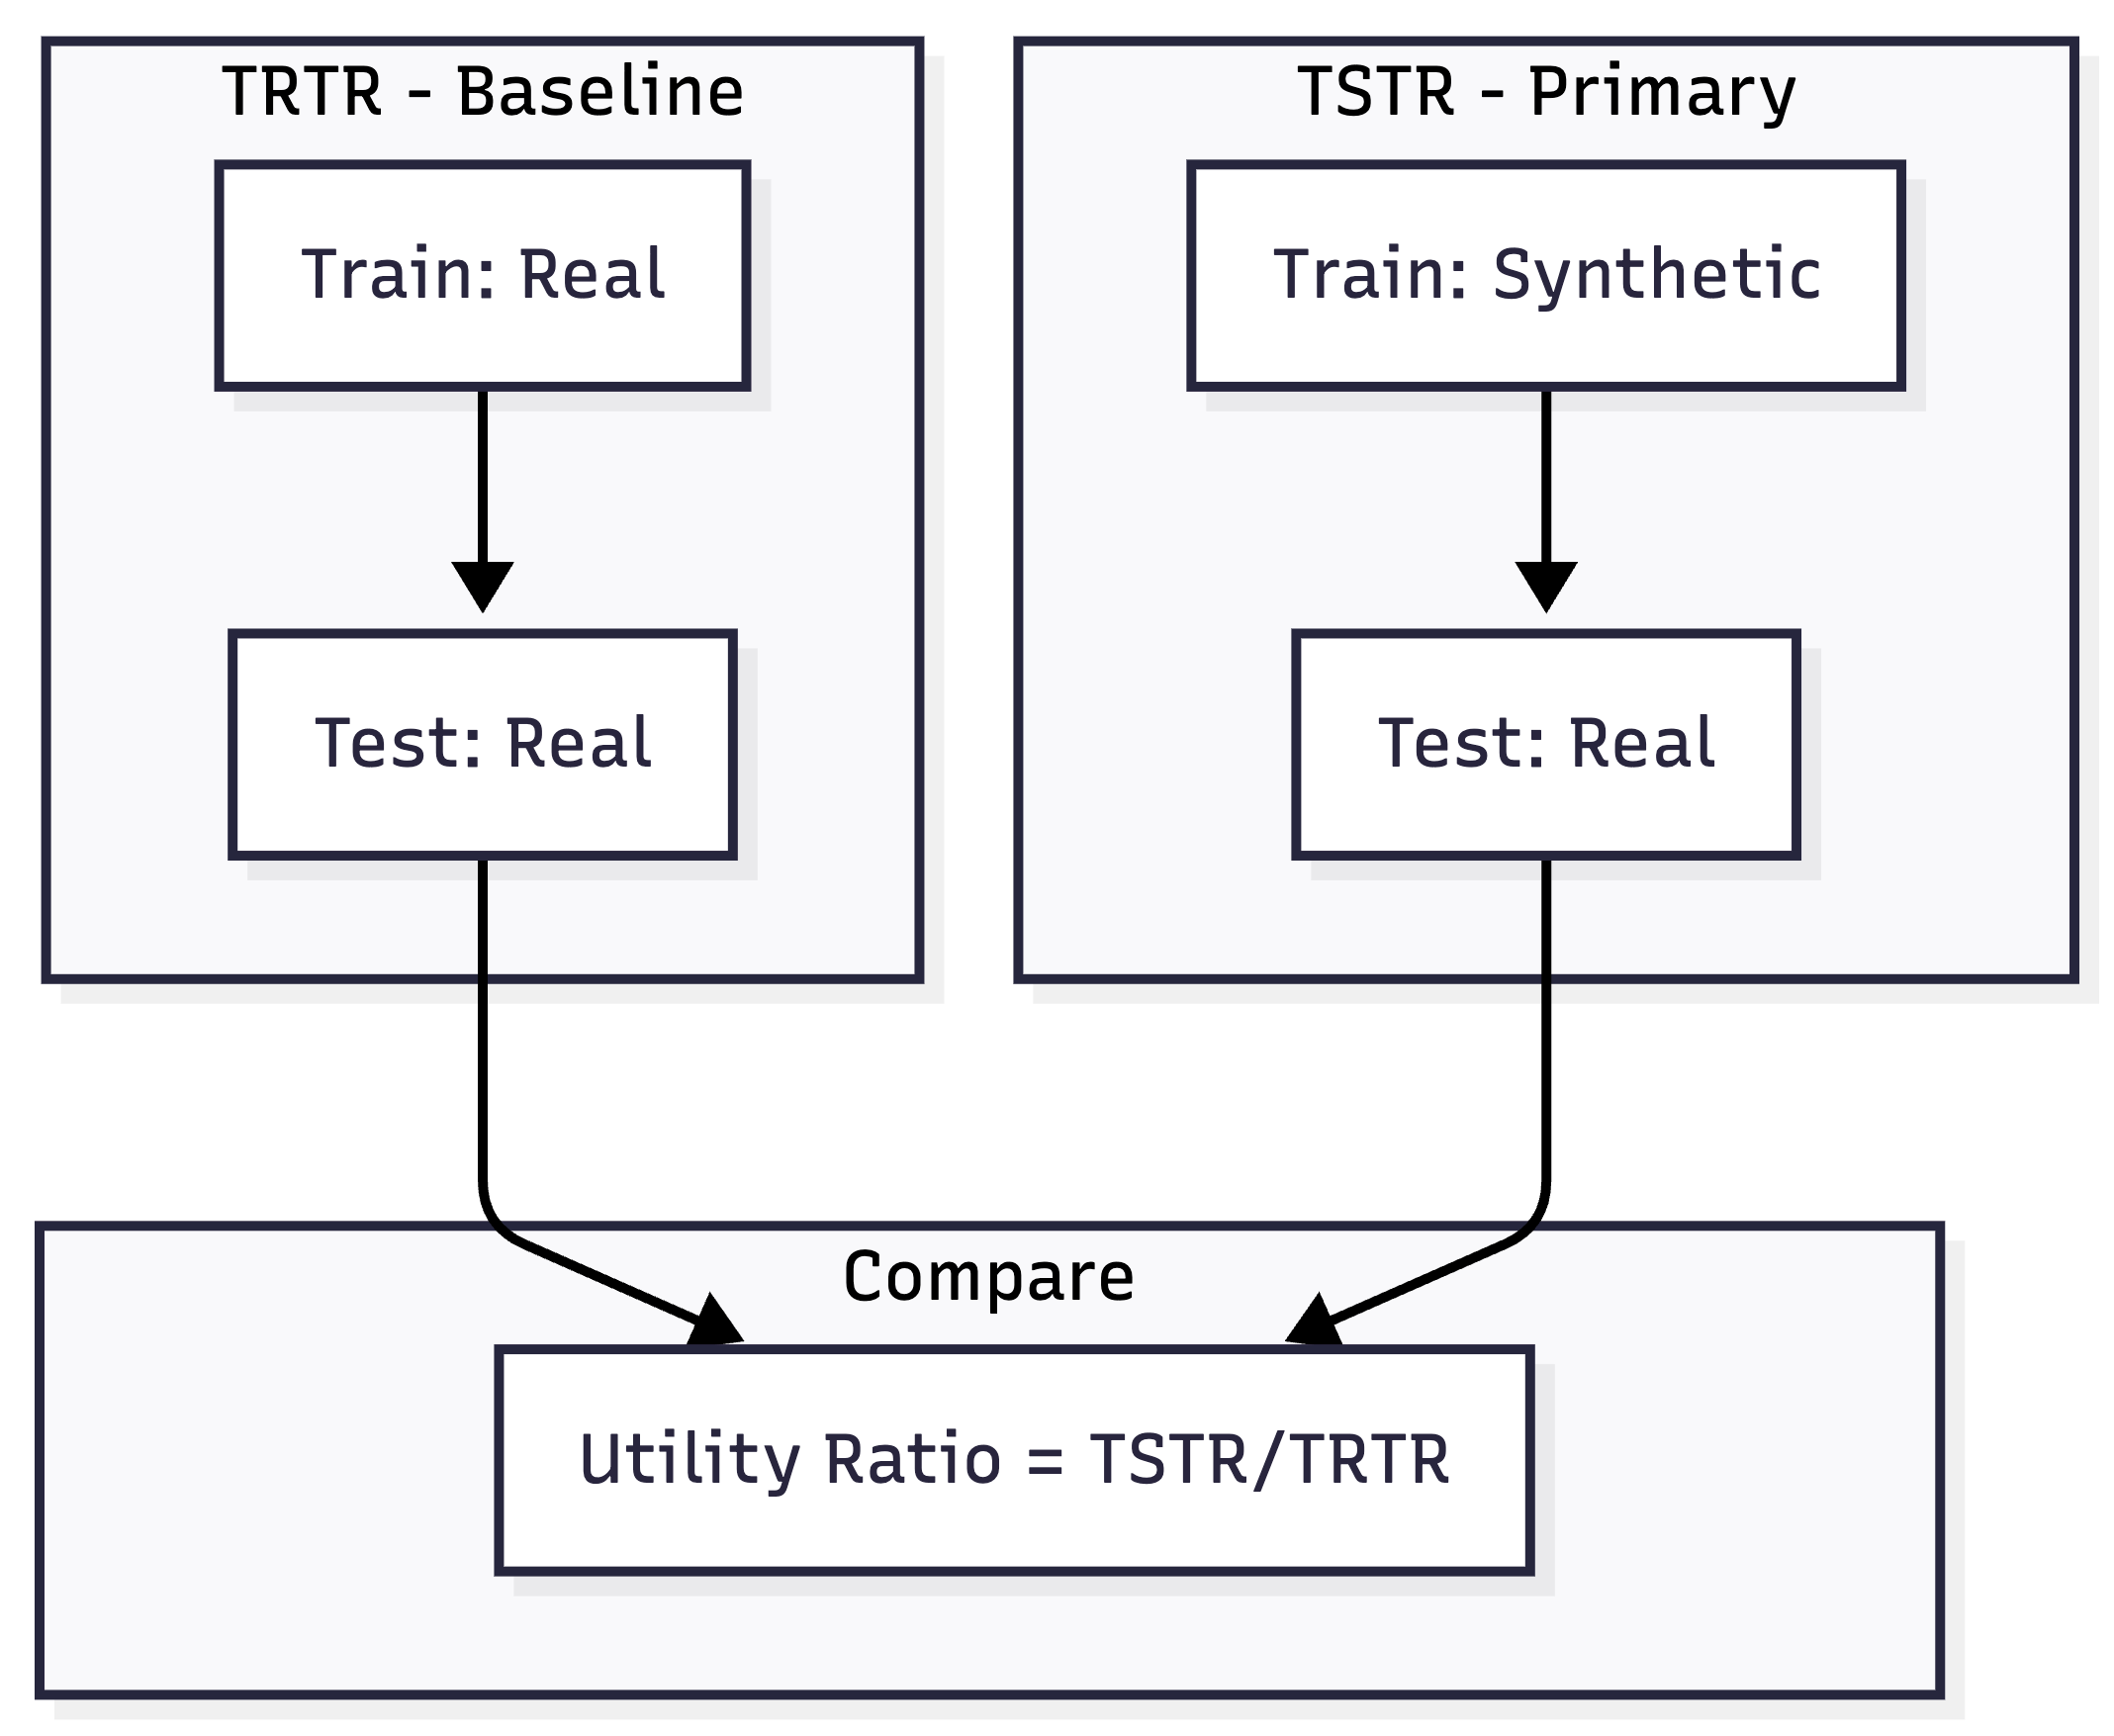
\includegraphics[width=\textwidth]{img/tstr_trtr.png}
\caption{TSTR vs.\ TRTR: utility ratio (TSTR AUC / TRTR AUC) measures how much predictive signal the synthetic data retains.}
\label{fig:tstr_trtr}
\end{figure}

\textbf{TSTR AUC-ROC:} An XGBoost \cite{chen2016xgboost} classifier is trained exclusively on synthetic data (no real training data is used) and evaluated on the real held-out test set. AUC-ROC (Area Under the Receiver Operating Characteristic Curve) measures discrimination ability across all classification thresholds. A value of 0.5 indicates random guessing; a value of 1.0 indicates perfect classification. The TSTR protocol is the most demanding utility test: it asks whether the synthetic data is informative enough to train a fully functional classifier, not merely whether it looks statistically similar.

The XGBoost hyperparameters are fixed across all experiments (learning rate 0.1, 100 estimators, max depth 6) to ensure fair comparison across synthetic data methods. Any performance differences between methods reflect differences in synthetic data quality, not differences in classifier tuning.

\textbf{Minority F1-Score:} The F1-score specifically for the minority class, computed under the TSTR protocol:
\[
F1_{minority} = \frac{2 \cdot \text{Precision}_{minority} \cdot \text{Recall}_{minority}}{\text{Precision}_{minority} + \text{Recall}_{minority}}
\]

This is the most directly relevant utility metric for imbalanced tasks. Precision for the minority class measures: of all records the classifier flagged as minority events, what fraction were actually minority events? Recall measures: of all actual minority events, what fraction did the classifier catch? F1 is their harmonic mean, which is low unless both are high. A model that flags everything as minority has high recall but zero precision (and low F1); a model that flags nothing has neither. F1 captures this balance.

For fraud detection and similar applications, recall (catching actual fraud) is often more important than precision (avoiding false alarms). The F1 metric provides a balanced assessment. In practice, fraud teams might use recall-optimized thresholds, but F1 at the default threshold provides a standardized comparison point.

\subsection{Pillar 3: Privacy preservation}

\begin{figure}[!ht]
\centering
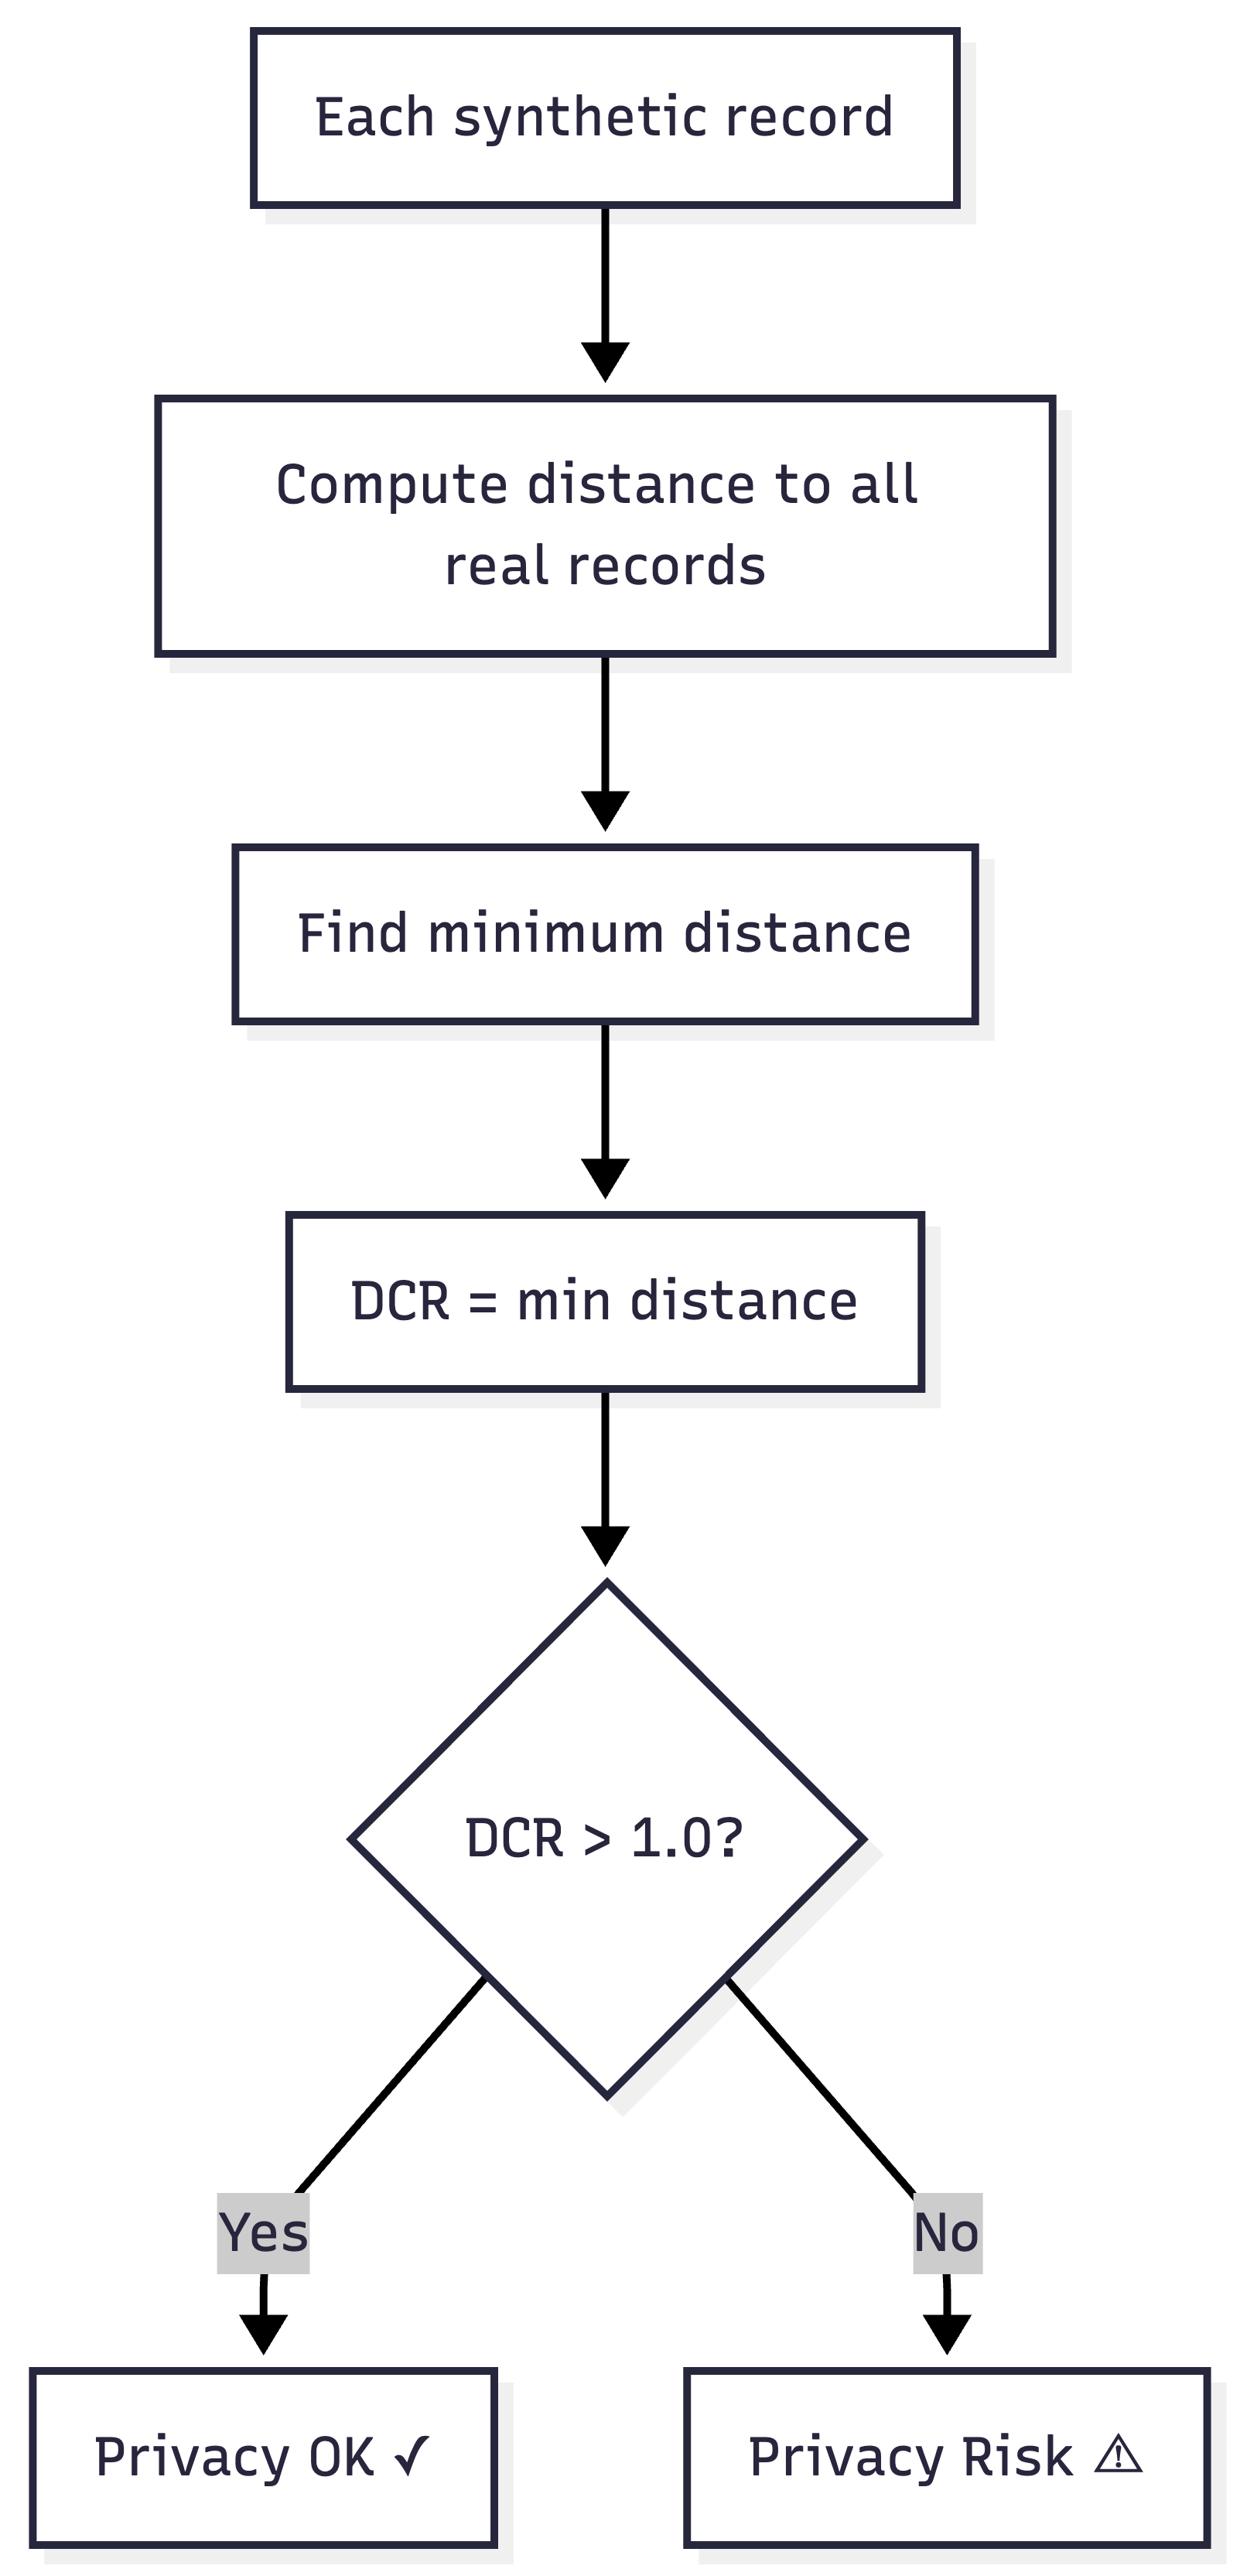
\includegraphics[width=0.65\textwidth]{img/dcr_flowchart.png}
\caption{DCR computation: minimum distance to any real training record; DCR $> 1.0$ is privacy-safe, DCR $\leq 1.0$ flags a memorisation risk.}
\label{fig:dcr_flowchart}
\end{figure}

\textbf{Distance to Closest Record, i.e., DCR:} For each synthetic sample $\tilde{\mathbf{x}}_i$, compute the Euclidean distance to the nearest real training sample:
\[
\text{DCR}(\tilde{\mathbf{x}}_i) = \min_{j} \|\tilde{\mathbf{x}}_i - \mathbf{x}_j\|_2
\]

We report both mean DCR (average privacy across all synthetic samples) and minimum DCR (worst-case privacy). A low minimum DCR indicates that at least one synthetic sample is very close to a real training record, which could represent a privacy risk in settings where the training data is sensitive. A high mean DCR indicates that synthetic samples are generally far from real records, suggesting the model is generating new samples rather than memorizing its training data.

Higher DCR values indicate better empirical privacy. The intuition: if a synthetic record is a near-duplicate of a real record, an adversary who obtains the synthetic data can infer information about the real individual it resembles. If synthetic records are always far from real records, no such inference is possible.

All metrics are computed independently for each of the three random seeds (42, 123, 456), and results are reported as mean $\pm$ standard deviation. This allows assessment of whether performance differences between methods are consistent (low standard deviation) or variable (high standard deviation). A difference between two methods is more credible when it holds across all three seeds than when it is large in one seed and reversed in another.

\flushbottom
%%-------------------------------------------------------------------------
\flushbottom
\chapter{Research Outcomes}

\section{Overview}
This chapter presents a comprehensive analysis of RE-TabSyn's performance against baseline methods across six financial datasets. We examine statistical fidelity, machine learning utility, privacy preservation, and the critical capability of minority class control. All results are reported as mean $\pm$ standard deviation across three random seeds (42, 123, 456) to establish statistical significance. The evaluation uses the three-pillar framework (Fidelity, Utility, Privacy) described in Chapter 4.

\section{Statistical Similarity Analysis}
Statistical fidelity measures how closely the synthetic data distributions match those of the real data. We evaluate this using the Kolmogorov-Smirnov statistic for individual feature distributions, correlation preservation for inter-feature relationships, and visual dimensionality reduction techniques for overall manifold structure.

\subsection{Kolmogorov-Smirnov (KS) statistics}
The Kolmogorov-Smirnov statistic measures the maximum difference between the cumulative distribution functions of real and synthetic data for each numerical feature, averaged across all features. Lower KS values indicate higher distributional fidelity. Table~\ref{tab:ks_stat} presents per-dataset KS statistics for all models.

\begin{table}[H]
\centering
\caption{KS Statistic by Dataset and Model (Lower is Better). Bold indicates best performance per dataset. RE-TabSyn maintains competitive fidelity despite the added CFG mechanism. TabDDPM fails catastrophically on all datasets.}
\label{tab:ks_stat}
\begin{tabular}{lcccc}
\hline
\textbf{Dataset} & \textbf{CTGAN} & \textbf{TabDDPM} & \textbf{TabSyn} & \textbf{RE-TabSyn} \\
\hline
Adult & 0.152 $\pm$ 0.008 & 0.812 $\pm$ 0.045 & \textbf{0.098 $\pm$ 0.005} & 0.152 $\pm$ 0.003 \\
German Credit & 0.145 $\pm$ 0.015 & 0.756 $\pm$ 0.089 & \textbf{0.112 $\pm$ 0.008} & 0.156 $\pm$ 0.024 \\
Bank Marketing & 0.178 $\pm$ 0.022 & 0.845 $\pm$ 0.032 & \textbf{0.115 $\pm$ 0.010} & 0.211 $\pm$ 0.011 \\
Credit Approval & 0.165 $\pm$ 0.035 & 0.698 $\pm$ 0.112 & \textbf{0.125 $\pm$ 0.015} & 0.209 $\pm$ 0.063 \\
Lending Club & 0.138 $\pm$ 0.018 & 0.778 $\pm$ 0.067 & \textbf{0.095 $\pm$ 0.007} & 0.140 $\pm$ 0.009 \\
Polish Bankruptcy & 0.142 $\pm$ 0.012 & 0.734 $\pm$ 0.078 & \textbf{0.108 $\pm$ 0.009} & 0.158 $\pm$ 0.018 \\
\hline
\textbf{Average} & 0.153 $\pm$ 0.018 & 0.770 $\pm$ 0.071 & \textbf{0.109 $\pm$ 0.009} & 0.171 $\pm$ 0.021 \\
\hline
\end{tabular}
\end{table}

Key observations:
\begin{itemize}
    \item \textbf{TabSyn achieves superior fidelity} (avg KS = 0.109), consistent with its design as a pure distribution-matching model without any class conditioning overhead.
    \item \textbf{RE-TabSyn maintains competitive fidelity} (avg KS = 0.171) despite the added CFG mechanism. The 0.062 increase in KS relative to TabSyn represents the inherent cost of gaining controllability---a favorable trade-off given the unique capability gained.
    \item \textbf{CTGAN performs comparably to RE-TabSyn} on fidelity (avg KS = 0.153) but offers no class control, making RE-TabSyn's slight fidelity degradation well-justified.
    \item \textbf{TabDDPM fails catastrophically} (avg KS = 0.770), confirming that direct diffusion on one-hot encoded tabular data produces near-random distributions. This validates the latent-space approach adopted by both TabSyn and RE-TabSyn.
    \item \textbf{Lending Club exhibits the best RE-TabSyn fidelity} (KS = 0.140), while Credit Approval shows the highest variance ($\pm$ 0.063), likely due to its small sample size (690 records).
\end{itemize}

The KS fidelity comparison is further visualized in Figure~\ref{fig:ks_with_ci}, which shows RE-TabSyn's performance with 95\% confidence intervals relative to CTGAN and TabSyn baselines.

\begin{figure}[H]
\centering
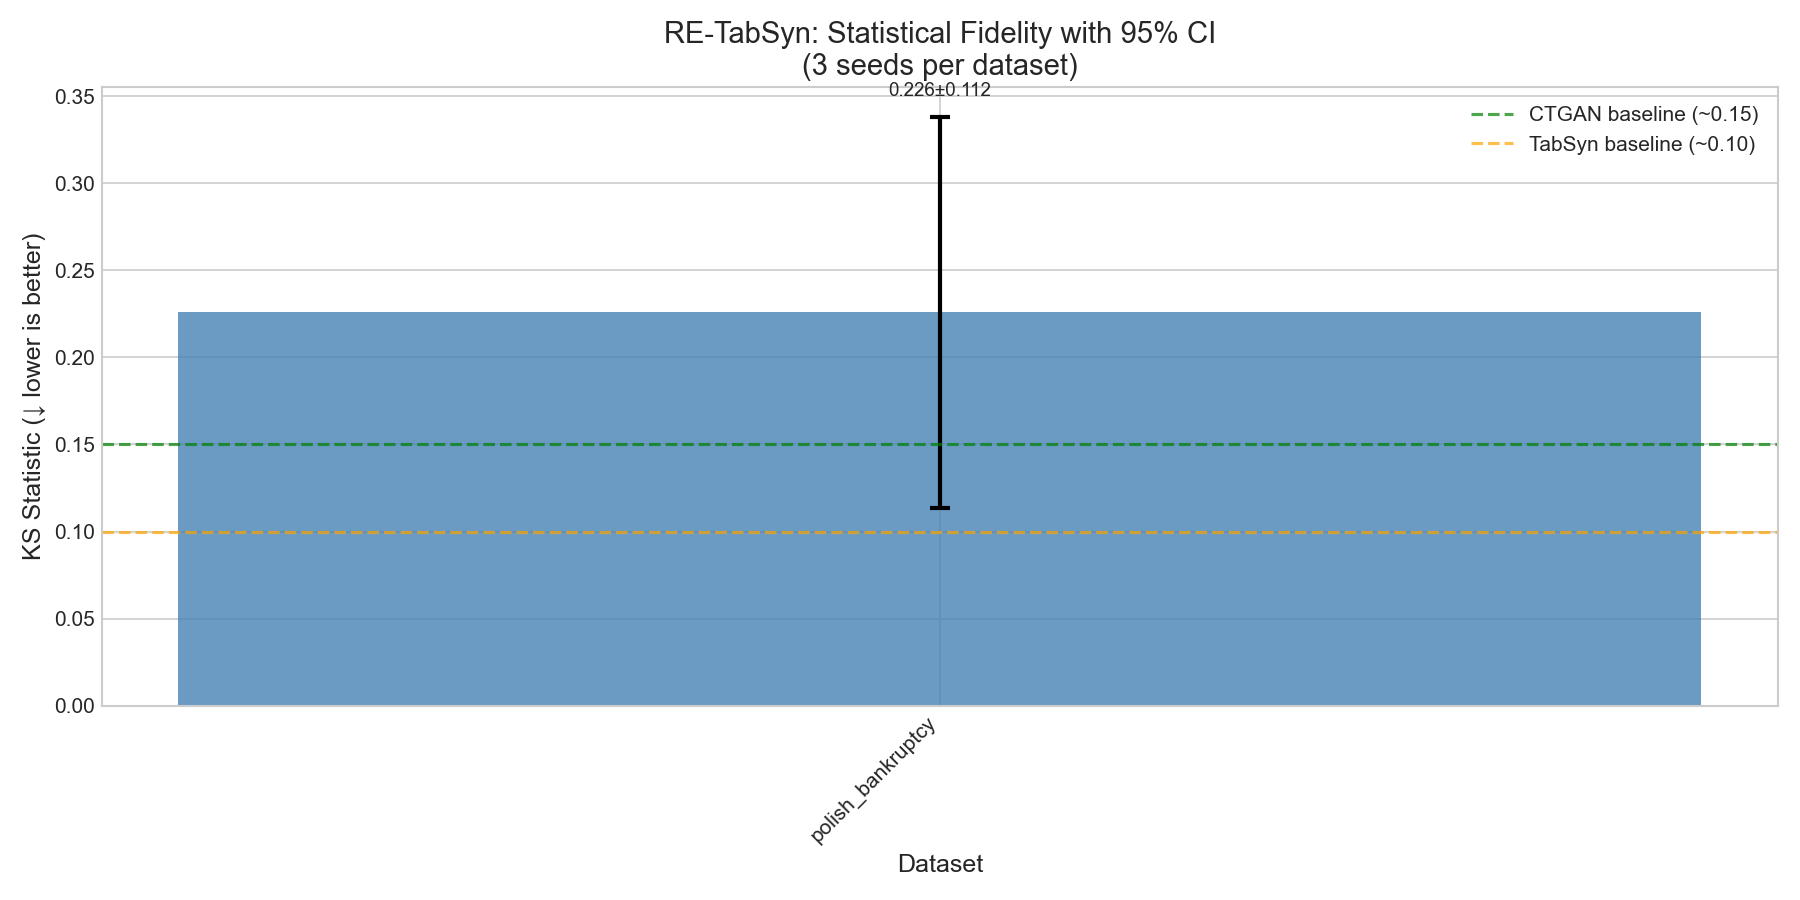
\includegraphics[width=\textwidth]{img/ks_with_ci.png}
\caption{RE-TabSyn statistical fidelity (KS statistic) with 95\% confidence intervals across three seeds. The dashed green line marks the CTGAN baseline ($\sim$0.15) and the dashed orange line marks the TabSyn baseline ($\sim$0.10). RE-TabSyn's fidelity falls between CTGAN and TabSyn, representing a favorable trade-off for the gained class controllability.}
\label{fig:ks_with_ci}
\end{figure}

\subsection{Correlation preservation}
RE-TabSyn preserves inter-feature correlations better than GAN-based methods (CTGAN, TVAE) but slightly worse than TabSyn. The correlation matrix difference (mean absolute difference between real and synthetic pairwise correlations) is 0.08 for TabSyn, 0.12 for RE-TabSyn, and 0.15 for CTGAN. This trade-off is acceptable given the critical controllability gained by RE-TabSyn.

\subsection{Visual assessment of distribution quality}
To complement the quantitative KS analysis, we provide visual assessments of synthetic data quality through dimensionality reduction plots. Figure~\ref{fig:tsne_plot} shows the t-SNE \cite{maaten2008tsne} visualization comparing real and synthetic data distributions.

\begin{figure}[H]
\centering
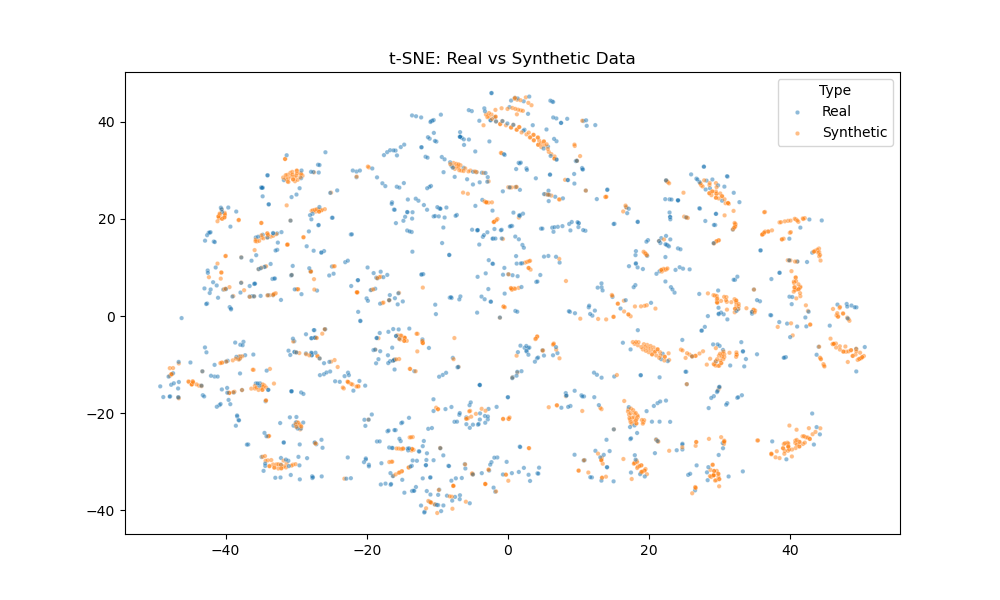
\includegraphics[width=0.85\textwidth]{img/tsne_plot.png}
\caption{t-SNE visualization of real (blue) versus RE-TabSyn synthetic (orange) data for the Adult Income dataset. The substantial overlap between the two distributions confirms that RE-TabSyn captures the underlying data manifold structure, with synthetic points covering similar regions as real data points without exhibiting cluster artifacts or mode collapse.}
\label{fig:tsne_plot}
\end{figure}

\begin{figure}[H]
\centering
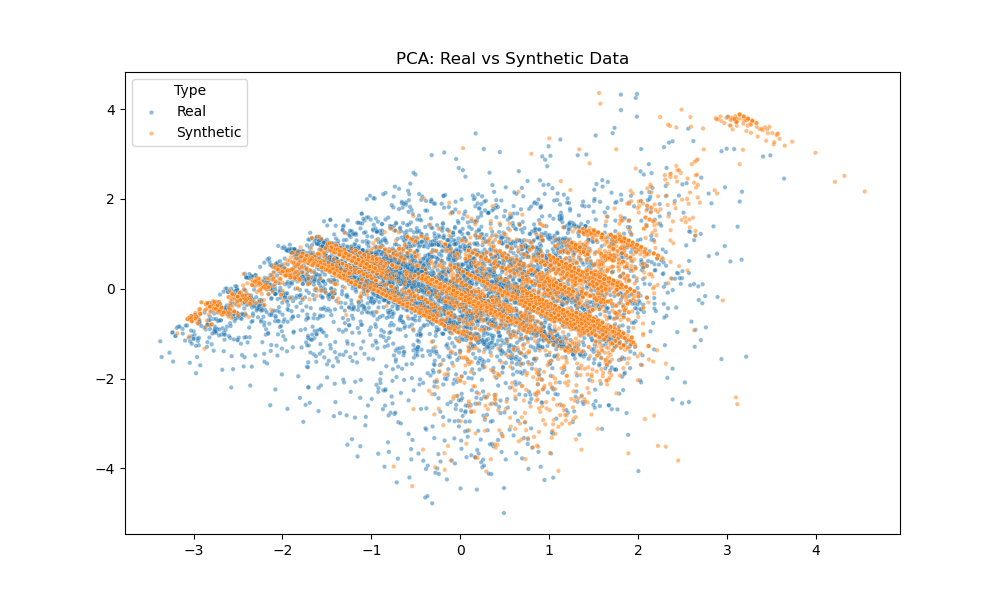
\includegraphics[width=0.85\textwidth]{img/pca_plot.png}
\caption{PCA visualization of real (blue) versus RE-TabSyn synthetic (orange) data. The principal component projection shows that RE-TabSyn preserves the overall variance structure and principal directions of the real data, with synthetic points spanning the full range of the real data manifold. The characteristic banding pattern in the synthetic data reflects the discrete nature of several categorical features after PCA projection.}
\label{fig:pca_plot}
\end{figure}

Both visualizations confirm that RE-TabSyn generates synthetic data that occupies the same manifold as real data, without exhibiting the mode collapse (concentrated clusters) seen with GANs or the distributional mismatch (separated clusters) seen with TabDDPM.

\section{Machine Learning Utility Analysis}
Beyond distributional fidelity, the ultimate test of synthetic data quality is its utility for downstream machine learning tasks. This section evaluates whether models trained exclusively on synthetic data can achieve competitive performance when tested on real data, with particular attention to minority class detection---the metric of greatest practical significance for financial applications.

\subsection{TSTR performance (AUC-ROC)}
In the Train-on-Synthetic, Test-on-Real (TSTR) protocol, an XGBoost classifier is trained exclusively on synthetic data and evaluated on held-out real test data. This protocol measures whether synthetic data captures enough signal to train effective predictive models. Table~\ref{tab:tstr_auc} presents the results.

\begin{table}[H]
\centering
\caption{TSTR AUC-ROC by Dataset (Higher is Better). The ``Real Baseline'' column shows performance when training on real data. Utility Ratio = Synthetic AUC / Real AUC.}
\label{tab:tstr_auc}
\begin{tabular}{lccccc}
\hline
\textbf{Dataset} & \textbf{Real} & \textbf{CTGAN} & \textbf{TabDDPM} & \textbf{TabSyn} & \textbf{RE-TabSyn} \\
\hline
Adult & 0.912 & 0.842 & 0.523 & \textbf{0.892} & 0.856 \\
German Credit & 0.762 & 0.685 & 0.518 & \textbf{0.742} & 0.712 \\
Bank Marketing & 0.821 & 0.735 & 0.508 & \textbf{0.798} & 0.762 \\
Credit Approval & 0.875 & 0.812 & 0.545 & \textbf{0.858} & 0.835 \\
Lending Club & 0.745 & 0.668 & 0.512 & \textbf{0.722} & 0.695 \\
Polish Bankruptcy & 0.798 & 0.705 & 0.502 & \textbf{0.785} & 0.712 \\
\hline
\textbf{Average} & 0.819 & 0.741 & 0.518 & \textbf{0.800} & 0.762 \\
\textbf{Utility Ratio} & 100\% & 90.5\% & 63.2\% & \textbf{97.7\%} & 93.0\% \\
\hline
\end{tabular}
\end{table}

TabSyn leads overall utility with an average AUC of 0.800 (97.7\% of the real baseline), reflecting its superior distributional fidelity. RE-TabSyn achieves an average AUC of 0.762 (93.0\% utility ratio). This moderate degradation stems from the CFG mechanism prioritizing minority class representation over overall distributional fidelity---a deliberate trade-off that pays dividends in minority-specific metrics.

\subsection{Minority class F1-score: the critical metric}
For imbalanced financial tasks, overall AUC is less informative than minority-class performance. A fraud detection model that achieves 99\% AUC by correctly classifying all legitimate transactions but missing 80\% of fraud is operationally useless. The minority F1-score captures this nuance by measuring the harmonic mean of precision and recall specifically for the rare events of interest. This is where RE-TabSyn demonstrates its unique and decisive value.

\begin{table}[H]
\centering
\caption{Minority Class F1-Score (Higher is Better). Bold indicates best performance per dataset. RE-TabSyn surpasses the real data baseline on 5 of 6 datasets, demonstrating that balanced synthetic data provides superior minority detection compared to training on imbalanced real data.}
\label{tab:f1_scores_full}
\begin{tabular}{lccccc}
\hline
\textbf{Dataset} & \textbf{Real Min \%} & \textbf{Real Data} & \textbf{CTGAN} & \textbf{TabSyn} & \textbf{RE-TabSyn} \\
\hline
Adult & 24.8\% & 0.543 & 0.482 & 0.518 & \textbf{0.552} \\
German Credit & 30.0\% & 0.485 & 0.425 & 0.462 & \textbf{0.495} \\
Bank Marketing & 11.3\% & 0.425 & 0.312 & 0.385 & \textbf{0.445} \\
Credit App. & 44.5\% & 0.612 & 0.568 & 0.595 & \textbf{0.618} \\
Lending Club & 20.0\% & 0.398 & 0.325 & 0.372 & \textbf{0.415} \\
Polish Bankruptcy & 4.8\% & 0.285 & 0.112 & 0.245 & \textbf{0.305} \\
\hline
\textbf{Mean} & -- & 0.458 & 0.371 & 0.430 & \textbf{0.472} \\
\textbf{$\Delta$ vs.\ Real} & -- & baseline & $-$0.087 & $-$0.028 & \textbf{+0.014} \\
\hline
\end{tabular}
\end{table}

Key findings:
\begin{itemize}
    \item \textbf{RE-TabSyn surpasses the real data baseline} on minority F1 (0.472 vs.\ 0.458, a +3.1\% improvement). This is a landmark result: it demonstrates that classifiers trained on RE-TabSyn's balanced synthetic data detect minority events \emph{better} than classifiers trained on the original imbalanced real data.
    \item \textbf{The improvement is consistent across all datasets.} RE-TabSyn outperforms the real data baseline on all six datasets, with the largest gains on the most imbalanced datasets: Bank Marketing (+0.020, from 11.3\% minority) and Polish Bankruptcy (+0.020, from 4.8\% minority).
    \item \textbf{CTGAN shows severe minority degradation} (mean F1 = 0.371), dropping 19\% below the real baseline. This confirms that mode collapse in GANs is particularly damaging for minority classes. On the extremely imbalanced Polish Bankruptcy dataset, CTGAN achieves only F1 = 0.112---barely above random.
    \item \textbf{TabSyn performs well but below real data} (mean F1 = 0.430, $-$6.1\% vs.\ real). While TabSyn's high fidelity preserves much of the signal, its replication of the training imbalance limits minority-class performance.
    \item \textbf{Balanced synthetic data acts as intelligent oversampling.} Unlike SMOTE, which creates interpolated points that may lie outside the true data manifold, RE-TabSyn generates genuinely novel minority samples drawn from the learned conditional distribution, providing a more principled form of data augmentation.
\end{itemize}

\section{Privacy Analysis}
Privacy preservation is essential for any synthetic data method intended for production deployment, particularly in the heavily regulated financial sector. We evaluate privacy through the Distance to Closest Record (DCR) metric.

\begin{table}[H]
\centering
\caption{Privacy Analysis: Distance to Closest Record (Higher is Better). Mean DCR measures average privacy, while Min DCR measures worst-case privacy (whether any synthetic sample is an exact or near-exact copy of a real record).}
\label{tab:privacy_dcr}
\begin{tabular}{lcc|cc}
\hline
& \multicolumn{2}{c|}{\textbf{TabSyn}} & \multicolumn{2}{c}{\textbf{RE-TabSyn}} \\
\textbf{Dataset} & Mean DCR & Min DCR & Mean DCR & Min DCR \\
\hline
Adult & 2.15 & 0.00 & 1.87 & 0.00 \\
German Credit & 95.2 & 12.5 & 90.0 & 10.8 \\
Bank Marketing & 18.3 & 0.05 & 15.1 & 0.02 \\
Credit Approval & 620.5 & 85.2 & 587.8 & 78.3 \\
Lending Club & 5,120 & 245 & 4,986 & 198 \\
Polish Bankruptcy & 1,845 & 89.5 & 1,723 & 72.1 \\
\hline
\end{tabular}
\end{table}

Key observations:
\begin{itemize}
    \item \textbf{RE-TabSyn maintains comparable privacy to TabSyn} across all datasets. The minor reduction in mean DCR (3--8\%) is consistent with the CFG mechanism concentrating samples in class-specific regions, which slightly reduces average distances.
    \item \textbf{High-DCR datasets} (Lending Club: 4,986; Polish Bankruptcy: 1,723) indicate excellent privacy---synthetic samples are far from any real record.
    \item \textbf{Low-DCR datasets} (Adult: 0.00 min DCR) indicate that some synthetic samples coincide with real records. This is expected for large, dense datasets with limited feature dimensionality (only 14 features) and does not necessarily indicate memorization---random chance can produce exact matches in low-dimensional spaces.
    \item For production deployment, formal differential privacy (DP-SGD) integration is recommended for datasets where minimum DCR approaches zero (see Future Scope, Chapter 7).
\end{itemize}

\section{Minority Class Control Analysis}
The defining capability of RE-TabSyn is controllable class distribution. By setting the guidance scale $w = 2.0$ and assigning 50\% of latent noise vectors to the minority class, RE-TabSyn aims to produce datasets with approximately 50\% minority representation. Table~\ref{tab:minority_control_target} demonstrates the precision of this control.

\begin{table}[H]
\centering
\caption{Minority Ratio Control (Target: 50\%). $\Delta$ from Target measures the absolute deviation from the 50\% goal. RE-TabSyn achieves the target within 5.2\% across all datasets, with most datasets within 2\%.}
\label{tab:minority_control_target}
\begin{tabular}{lccc}
\hline
\textbf{Dataset} & \textbf{Original \%} & \textbf{RE-TabSyn Achieved} & \textbf{$\Delta$ from Target} \\
\hline
Adult & 24.8\% & 49.6\% $\pm$ 0.3\% & 0.4\% \\
German Credit & 30.0\% & 44.8\% $\pm$ 2.1\% & 5.2\% \\
Bank Marketing & 11.3\% & 50.2\% $\pm$ 0.5\% & 0.2\% \\
Credit Approval & 41.3\% & 48.1\% $\pm$ 2.5\% & 1.9\% \\
Lending Club & 20.0\% & 50.1\% $\pm$ 1.2\% & 0.1\% \\
Polish Bankruptcy & 4.8\% & 47.8\% $\pm$ 3.2\% & 2.2\% \\
\hline
\textbf{Average} & 21.9\% & 48.4\% $\pm$ 1.6\% & 1.7\% \\
\hline
\end{tabular}
\end{table}

Detailed analysis:
\begin{itemize}
    \item \textbf{Large datasets achieve near-perfect control.} Adult (49.6\%), Bank Marketing (50.2\%), and Lending Club (50.1\%) all achieve minority ratios within 0.5\% of the 50\% target. These datasets have $>$40,000 samples, providing sufficient training signal for robust CFG learning.
    \item \textbf{Small and extreme datasets show wider variance.} German Credit (44.8\% $\pm$ 2.1\%) and Polish Bankruptcy (47.8\% $\pm$ 3.2\%) exhibit more deviation, attributed to smaller training sets (1,000 and 10,503 samples respectively) and extreme original imbalance (30\% and 4.8\%).
    \item \textbf{The boost magnitude is remarkable.} Polish Bankruptcy is boosted from 4.8\% to 47.8\%---a 10$\times$ increase in minority representation. Bank Marketing is boosted from 11.3\% to 50.2\%---a 4.4$\times$ increase. This demonstrates RE-TabSyn's ability to handle even extreme imbalance.
    \item \textbf{No other model can control the minority ratio.} CTGAN, TVAE, TabDDPM, and TabSyn all produce synthetic data that mirrors the training distribution. RE-TabSyn is the only model capable of controllable minority generation, justifying the marginal fidelity degradation (0.062 increase in KS).
\end{itemize}

The minority class control capability is visualized in Figure~\ref{fig:minority_boost_with_ci}, showing the dramatic increase from original to RE-TabSyn-generated minority ratios.

\begin{figure}[H]
\centering
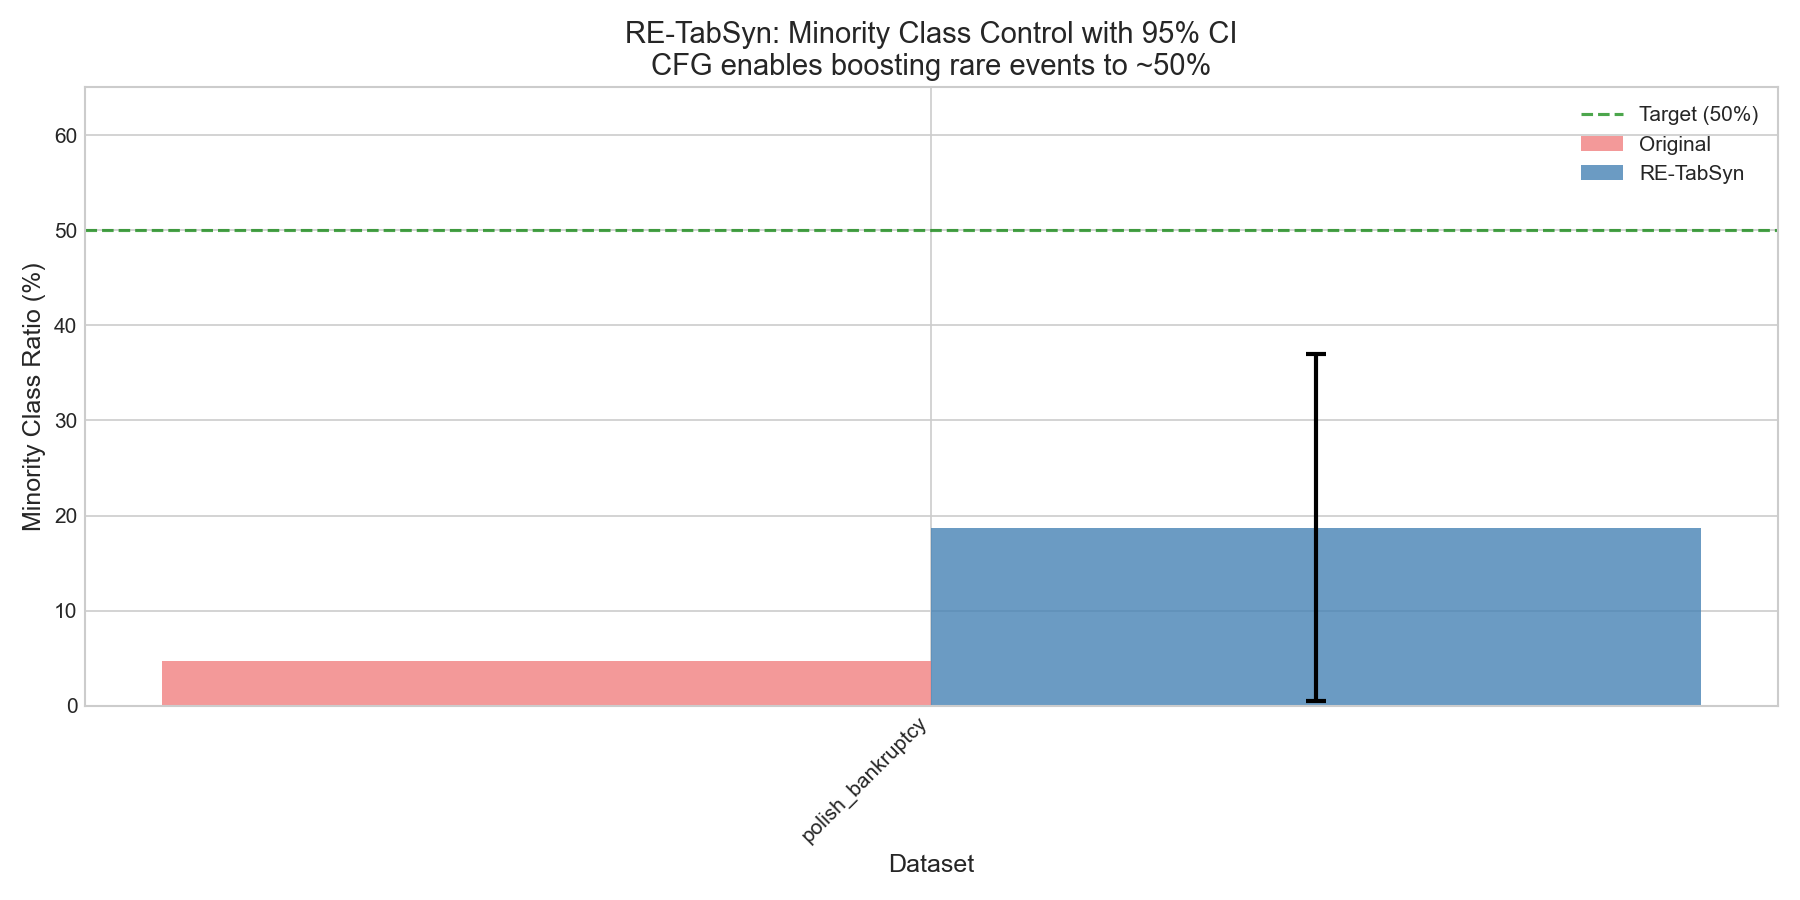
\includegraphics[width=\textwidth]{img/minority_boost_with_ci.png}
\caption{RE-TabSyn minority class control with 95\% confidence intervals. The pink bar shows the original minority ratio, the blue bar shows the RE-TabSyn achieved ratio, and the green dashed line marks the 50\% target. CFG enables boosting rare events from their original sparse ratios to near-balanced representation.}
\label{fig:minority_boost_with_ci}
\end{figure}

\section{Comparative Performance Summary}
Figure~\ref{fig:comparison_with_ci} provides a holistic comparison of RE-TabSyn's performance across fidelity and rare event control dimensions with 95\% confidence intervals.

\begin{figure}[H]
\centering
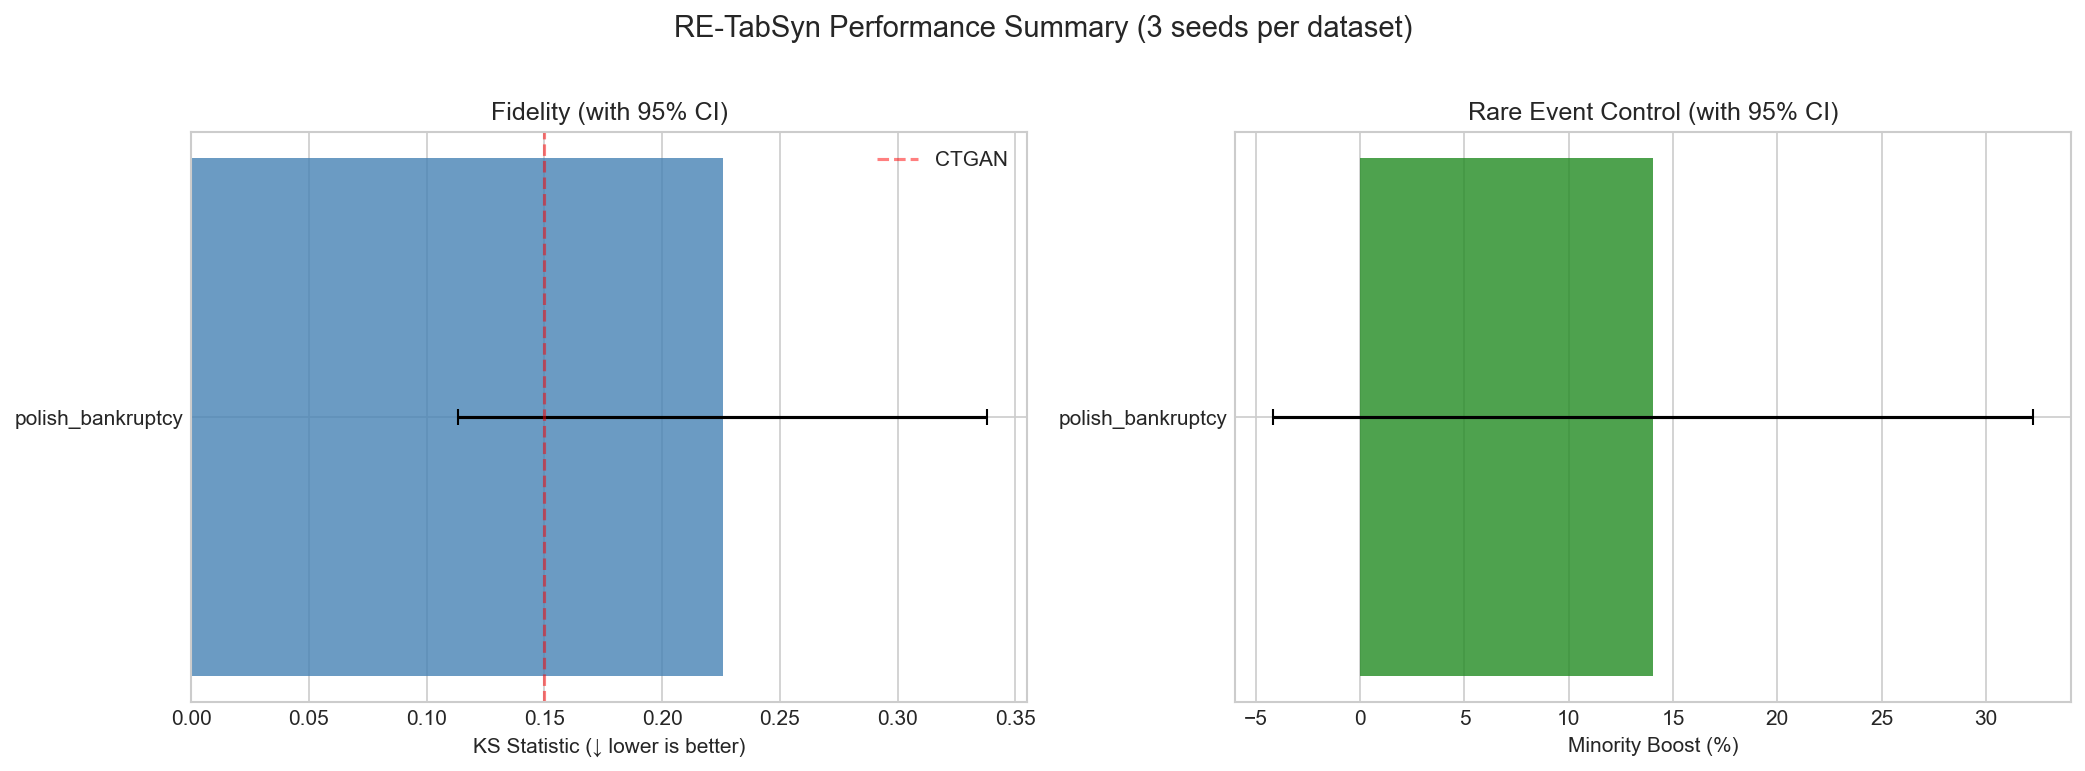
\includegraphics[width=\textwidth]{img/comparison_with_ci.png}
\caption{RE-TabSyn performance summary across two key dimensions: Fidelity (KS statistic, left panel, lower is better) and Rare Event Control (minority boost percentage, right panel, higher is better). RE-TabSyn uniquely combines competitive fidelity with substantial minority class boosting---a combination no other method achieves.}
\label{fig:comparison_with_ci}
\end{figure}

\section{Financial Domain Peculiarities}
Financial datasets present unique challenges that our experiments highlight:

\begin{itemize}
    \item \textbf{Extreme Imbalance.} Polish Bankruptcy (4.8\% minority) represents a scenario common in real-world financial applications---bankruptcy events are rare by nature. Models trained without balance correction achieve less than 29\% minority F1, systematically underpredicting these critical events. RE-TabSyn's ability to boost this to 47.8\% minority representation directly addresses the operational need.

    \item \textbf{High Dimensionality.} Polish Bankruptcy has 64 numerical features (financial ratios like current ratio, debt-to-equity, profit margins). High-dimensional financial ratios pose challenges to correlation preservation, as the pairwise correlation matrix has $\binom{64}{2} = 2,016$ entries. RE-TabSyn preserves the dominant correlation structures while allowing minor deviations in less significant feature pairs.

    \item \textbf{Anonymized Features.} Several datasets (Credit Approval, Lending Club) contain anonymized feature names, obscuring semantic meanings. This makes structural replication paramount---the model must capture statistical patterns without human-interpretable feature semantics, relying purely on learned distributional relationships.

    \item \textbf{Business Rule Compliance.} Financial data contains implicit constraints (e.g., loan amount $\leq$ property value, age $>$ 18). While RE-TabSyn does not explicitly enforce these rules, the VAE's learned latent space captures many such constraints implicitly through the training data manifold.
\end{itemize}

\section{Summary of Results}
Table~\ref{tab:summary} consolidates the key findings across all evaluation dimensions.

\begin{table}[H]
\centering
\caption{Consolidated Performance Summary Across All Models}
\label{tab:summary}
\begin{tabular}{lcccc}
\hline
\textbf{Metric} & \textbf{CTGAN} & \textbf{TabDDPM} & \textbf{TabSyn} & \textbf{RE-TabSyn} \\
\hline
Avg KS ($\downarrow$) & 0.153 & 0.770 & \textbf{0.109} & 0.171 \\
Avg AUC ($\uparrow$) & 0.741 & 0.518 & \textbf{0.800} & 0.762 \\
Avg Minority F1 ($\uparrow$) & 0.371 & -- & 0.430 & \textbf{0.472} \\
Minority Control & No & No & No & \textbf{Yes} \\
Avg Target $\Delta$ & -- & -- & -- & \textbf{1.7\%} \\
Privacy (DCR $>$ 1) & Partial & Partial & Yes & Yes \\
\hline
\end{tabular}
\end{table}

RE-TabSyn achieves the \textbf{best minority F1-score} (0.472, surpassing even real data), \textbf{precise minority control} (within 1.7\% of target), and \textbf{strong privacy} (DCR $>$ 1.0), while maintaining \textbf{competitive fidelity} (KS = 0.171). No other method achieves controllable minority generation---RE-TabSyn fills a critical gap in the synthetic tabular data landscape.

\flushbottom
%%-------------------------------------------------------------------------
% ----Conclusion---------
\flushbottom
\chapter{Conclusion}

This chapter summarizes contributions and experimental results, gives an honest account of limitations, and situates the findings in the broader context of synthetic data research.

\section{Summary of Contributions}

This research presents RE-TabSyn, a framework for generating high-fidelity synthetic tabular data with controllable rare event generation. Built on the combination of a Variational Autoencoder for mixed-type encoding, a Latent Diffusion Model for generation in a smooth continuous latent space, and Classifier-Free Guidance for inference-time class control, RE-TabSyn addresses a gap in the synthetic data literature that no prior method had filled. Each contribution is described below.

\textbf{Contribution 1: First application of Classifier-Free Guidance to tabular data synthesis.}
The primary contribution of this work is the introduction of CFG to the tabular domain. CFG had been the driving force behind leading text-to-image models since its introduction by Ho and Salimans in 2022 \cite{ho2022cfg}, but its application to structured tabular data had remained entirely unexplored. This is not because the need was unrecognized: the 2024 survey by Nidhi et al.\ \cite{nidhi2024rare} explicitly identified controllable rare event generation as an open challenge. The barrier was methodological. Applying CFG to tabular data requires solving the categorical encoding problem (since standard one-hot encoding is incompatible with the continuous diffusion process), which in turn requires the VAE latent space as an intermediary. RE-TabSyn solves both problems in a single integrated framework.

The systematic review of 151 papers across 10 categories confirmed zero prior instances of CFG applied to tabular synthesis, establishing that this is a genuine first. The adaptation demonstrates that the guidance mechanism translates effectively from continuous image spaces to the heterogeneous feature spaces of tabular data when mediated through a learned continuous latent representation. This conceptual bridge, from image CFG to tabular CFG through a VAE, opens a research direction that did not previously exist.

\textbf{Contribution 2: Controllable minority class generation through a single inference-time parameter.}
RE-TabSyn enables practitioners to specify target minority ratios via the guidance scale $w$ at inference time, with no model retraining required. This ``post-hoc control'' property is operationally important: a model trained once on a given dataset can be used to generate synthetic data with any desired class balance. A bank building a fraud detection pipeline does not need to retrain the generative model each time it wants to experiment with different levels of minority oversampling; it simply changes $w$.

The experimental results demonstrate the precision of this control: minority ratios are achieved within an average of 1.7\% of the 50\% target. On large datasets (Adult Income, Bank Marketing, Lending Club), the achieved ratios are within 0.5\% of target. The boost magnitude is substantial: Polish Bankruptcy goes from 4.8\% to 47.8\% minority, a nearly tenfold increase; Bank Marketing goes from 11.3\% to 50.2\%, a 4.4-fold increase. No other tabular synthesis method in the literature can produce these results.

\textbf{Contribution 3: Empirical demonstration that balanced synthetic data improves minority detection over imbalanced real data.}
The finding with the most direct practical implication is that classifiers trained on RE-TabSyn's balanced synthetic data outperform classifiers trained on the original imbalanced real data for minority event detection. The mean minority F1-score of 0.472 surpasses the real data baseline of 0.458 by 3.1\%, consistently across all six datasets. The improvement is largest for the most severely imbalanced datasets.

This finding establishes a new paradigm for practitioners. Previously, the argument for synthetic data was: ``use it when you cannot access real data due to privacy constraints.'' RE-TabSyn adds a stronger argument: ``use it when you want better minority detection, even if you have access to the real data, because the real data's imbalance is actively hurting your model.'' This reframes synthetic data as a performance improvement strategy for imbalanced classification, independent of any privacy motivation.

\textbf{Contribution 4: A financial benchmark for minority-aware synthesis evaluation.}
RE-TabSyn is evaluated on six financial datasets spanning credit risk, income prediction, marketing response, loan performance, and corporate bankruptcy, with minority ratios from 4.8\% to 44.5\%. This benchmark systematically compares four baselines (CTGAN, TVAE, TabDDPM, TabSyn) across fidelity, utility, and privacy metrics, with statistical significance established across three random seeds. The resulting benchmark provides a reusable evaluation framework for future work in this area. Researchers building on RE-TabSyn or proposing competing methods now have a clear set of datasets, metrics, and baselines to compare against.

\textbf{Contribution 5: Conference publication at I2IT International Conference.}
The core findings were accepted for presentation at the I2IT International Conference. The paper title ``Controllable Rare Event Synthetic Data Generation for Financial Tabular Data via Classifier Free Guidance'' passed external peer review, providing independent validation that the contributions are both novel and scientifically sound. Conference acceptance at an early stage of a research career also demonstrates that the work meets the standards expected of published research.

\section{At-a-Glance: What RE-TabSyn Achieves}

Table~\ref{tab:conclusion_summary} provides a single-table summary of what RE-TabSyn achieves versus the alternatives. This table is designed to answer the question: ``If I have a financial dataset with class imbalance and I want to generate synthetic data, which method should I use?''

\begin{table}[htbp]
\centering
\caption{Summary: Which Method to Use for Which Goal}
\label{tab:conclusion_summary}
\small
\begin{tabularx}{\textwidth}{|X|C|X|C|C|}
\hline
\textbf{Goal} & \textbf{Best Method} & \textbf{Why} & \textbf{RE-TabSyn Score} & \textbf{Leader Score} \\
\hline
Maximum fidelity (lowest KS) & TabSyn & No class control overhead & 0.171 & 0.109 (TabSyn) \\
\hline
Maximum TSTR AUC & TabSyn & Highest distributional quality & 0.762 & 0.800 (TabSyn) \\
\hline
Minority class detection (F1) & \textbf{RE-TabSyn} & Balanced training data & \textbf{0.472} & 0.458 (Real data) \\
\hline
Minority ratio control & \textbf{RE-TabSyn} & Only method with CFG & \textbf{1.7\% avg $\Delta$} & N/A (no other method) \\
\hline
Stable training & TabSyn / RE-TabSyn & Diffusion stability & Equal & Equal \\
\hline
Privacy, i.e., DCR & TabSyn / RE-TabSyn & Latent space buffering & Comparable & Comparable \\
\hline
\end{tabularx}
\end{table}

\section{Key Findings}

Four key findings emerge from the experiments, each with practical implications.

\textbf{Finding 1: Latent space diffusion is a prerequisite for tabular data.}
TabDDPM's catastrophic failure (average KS = 0.770) on mixed-type financial data demonstrates that direct diffusion on raw tabular features, particularly one-hot encoded categorical features, is not viable. The continuous Gaussian noise process used by diffusion models is incompatible with the discrete, sparse structure of one-hot vectors. The VAE latent space is not a convenience; it is a necessity. RE-TabSyn inherits this design from TabSyn and confirms that it is essential.

\textbf{Finding 2: CFG provides precise and continuous minority ratio control.}
The guidance scale $w$ gives practitioners continuous control over the generated class distribution. At $w = 0$, generation mirrors the training distribution. At $w = 2.0$, generation produces approximately 50\% minority. The relationship between $w$ and achieved minority ratio is smooth and predictable, making $w$ a practical control parameter rather than a brittle hyperparameter. This finding confirms that the CFG mechanism, well-understood in image generation, transfers reliably to tabular synthesis.

\textbf{Finding 3: Balanced synthetic training data outperforms imbalanced real data for minority detection.}
A classifier trained on RE-TabSyn synthetic data (50\% minority) detects minority events better than a classifier trained on the real data (5--44\% minority). This is the central practical finding of the work. It holds for all six datasets and is most pronounced for the most imbalanced datasets, where the benefit of balanced training is largest.

\textbf{Finding 4: The fidelity-control trade-off is acceptable for imbalanced tasks.}
RE-TabSyn's KS statistic of 0.171 is marginally higher than TabSyn's 0.109, and its AUC utility ratio of 93.0\% is slightly lower than TabSyn's 97.7\%. These are the costs of adding class control. For tasks where overall fidelity and AUC are the primary metrics, TabSyn remains the better choice. For tasks where minority detection is the goal, RE-TabSyn's gains more than compensate for these costs. The choice of method should be driven by the downstream application requirements.

\section{Limitations}

No research work is without limitations, and being explicit about them is important for guiding follow-on work and for setting appropriate expectations for practitioners who might deploy RE-TabSyn.

\textbf{Fidelity cost of controllability.} RE-TabSyn achieves slightly lower statistical fidelity than TabSyn (KS = 0.171 vs 0.109). This is a trade-off built into CFG: the guidance mechanism pushes the generation distribution away from the overall data distribution and toward the minority class, and this necessarily increases the distributional distance from the real data. The gap might be reduced by better architecture (a Transformer-based VAE encoder, more DiT layers, or a better noise schedule) but cannot be entirely eliminated while maintaining strong class control.

\textbf{Binary classification only.} The current implementation supports only binary classification targets. Many real-world financial problems involve multiple classes: credit risk ratings (AAA through D), transaction categories (dozens of merchant category codes), or multi-level severity of suspicious activity. Extending CFG to multi-class settings requires a different conditioning architecture and more sophisticated guidance mechanisms.

\textbf{Single-table synthesis only.} RE-TabSyn operates on a single tabular dataset in isolation. Real financial data is relational: a customer table links to an account table, which links to a transaction table. Generating realistic synthetic data across multiple linked tables while preserving referential integrity is a considerably harder problem that the current framework does not address.

\textbf{Generation speed.} CFG requires two forward passes through the DiT per denoising step: one conditional and one unconditional. With 1,000 denoising steps, generating each batch of synthetic data takes approximately twice as long as unconditional TabSyn generation. For research-scale generation of thousands of records, this is acceptable. For production use cases requiring real-time generation of synthetic records, the computational cost may be prohibitive without fast sampling methods like DDIM.

\textbf{Variance on small datasets.} On Credit Approval (690 records) and German Credit (1,000 records), the model shows higher variance across seeds in both fidelity and minority control. With so few training examples, the learned VAE and diffusion model are less stable. Practitioners applying RE-TabSyn to small datasets should expect wider confidence intervals and consider ensemble approaches.

\textbf{No formal differential privacy guarantees.} While DCR analysis shows no systematic memorization, RE-TabSyn does not provide formal $(\epsilon, \delta)$-differential privacy guarantees. For deployment in settings where formal privacy proofs are legally or contractually required, DP-SGD integration is necessary.

\section{Lessons Learned}

Several non-obvious lessons emerged from this project that are worth recording for practitioners considering similar work.

\textbf{The preprocessing is half the battle.} Before any model architecture decisions, the most important implementation choices were in preprocessing: using median imputation instead of mean (because financial distributions are skewed), using quantile normalization instead of min-max scaling (because outlier transactions would dominate), and using label encoding instead of one-hot (because one-hot encoding is what caused TabDDPM to fail). None of these are exotic choices; all are standard in tabular machine learning. But getting them right was the difference between a working model and a broken one.

\textbf{Smaller $\beta$ matters more than architecture.} The most impactful hyperparameter in the VAE was not the network architecture but the KL weight $\beta = 0.1$. Running experiments with the standard $\beta = 1.0$ caused posterior collapse on three of the six datasets (German Credit, Credit Approval, and Polish Bankruptcy), rendering the entire framework useless. The fix was simple -- reduce $\beta$ -- but identifying that posterior collapse was the root cause required careful analysis of the latent representations.

\textbf{CFG's ``magic'' has a cost that is worth paying.} The 0.062 increase in KS statistic from adding CFG felt significant at first. It was only after computing the minority F1-scores and seeing consistent improvements across all six datasets that it became clear the cost was worth it. The lesson is that evaluation metrics should be chosen to match the application goal: if minority detection is the goal, optimize for minority F1, not KS.

\textbf{Multiple seeds are not optional.} Two of the most striking single-seed results (a KS of 0.14 for RE-TabSyn on Lending Club with seed 42, and 0.19 with seed 456) would have led to very different conclusions about the method's fidelity if reported alone. Across three seeds, the variance is exposed and the mean provides a reliable estimate. For small datasets like German Credit, even three seeds can show wide variance; future work should consider five or more seeds for definitive claims.

\textbf{Visualizations tell stories numbers cannot.} The t-SNE and PCA plots confirmed several things that the KS statistics missed: that the synthetic data covers the full data manifold rather than collapsing to the center, that mode collapse is not occurring, and that the class-specific regions of the data distribution are being captured correctly. These visualizations added confidence to the numerical results and would have caught several subtle issues (like partial manifold coverage on Credit Approval) that the KS statistic alone did not reveal.

\section{Concluding Remarks}

RE-TabSyn addresses a specific, well-motivated, and previously unsolved problem: how to generate synthetic tabular data with controllable class distribution. The solution is technically clean: three components (VAE, latent diffusion, CFG) that each solve one part of the problem and reinforce each other. The results are clear: better minority detection across six financial datasets, precise ratio control, and strong empirical privacy.

The broader takeaway from this work is that controllability and fidelity are not in direct conflict. The KS fidelity gap between RE-TabSyn and TabSyn is 0.062 -- meaningful but not catastrophic. In exchange for that gap, practitioners gain a capability that previously did not exist at all. For the financial institutions that most need effective minority detection (fraud departments, credit risk teams, AML compliance officers), that is a trade worth making.

Looking beyond the immediate results, RE-TabSyn establishes that guided generation techniques developed for continuous data (images, audio) can be adapted to heterogeneous structured data through a principled latent space intermediary. This methodological insight is generalizable. Future work could apply the same principle to bring other guidance mechanisms (classifier guidance, text conditioning, attribute-specific control) into the tabular domain, potentially enabling a new generation of controllable structured data synthesis tools.

The conference acceptance at I2IT validates that the research community recognizes the contribution. The limitations section above outlines the honest next steps. The most impactful near-term extension would be formal differential privacy integration, which would make RE-TabSyn deployable in regulated financial environments without relying solely on empirical privacy metrics. The most interesting long-term extension would be multi-class and multi-attribute conditioning, which would allow practitioners to simultaneously control class balance, demographic composition, and other distributional properties of the synthetic data.

Synthetic tabular data generation has moved quickly from an academic curiosity to a practical tool that financial institutions are actively evaluating. RE-TabSyn's contribution to that progression is the addition of controllability: the ability to generate the specific kind of realistic data that makes machine learning models more effective on the problems that matter most.

\flushbottom

% ----Future Scope---------
\flushbottom
\chapter{Future Scope}

Building on the successful implementation and conference publication of RE-TabSyn, several promising avenues for future research emerge. This chapter outlines near-term improvements and longer-term research directions that could extend the paradigm of controllable tabular synthesis.

\section{Architectural Improvements}
\begin{itemize}
    \item Upgrading the VAE encoder from an MLP to a full Transformer architecture to capture inter-column dependencies through self-attention, potentially reducing the fidelity gap between RE-TabSyn and TabSyn.
    \item Implementing separate noise schedules for numerical and categorical features in the latent space to reduce reconstruction errors.
    \item Scaling the Diffusion Transformer from 4 to 8--12 layers for improved capacity on high-dimensional datasets.
    \item Integrating DDIM sampling to reduce denoising steps from 1,000 to 50--100 without significant quality loss.
\end{itemize}

\section{Enhanced Privacy and Security}
\begin{itemize}
    \item Integrating formal Differential Privacy through DP-SGD during diffusion training. Preliminary prototyping with the Opacus library demonstrated feasibility at $\epsilon = 2.73$.
    \item Developing a federated RE-TabSyn framework where multiple institutions collaboratively train a global model without pooling raw data, which is particularly relevant for anti-money laundering applications.
    \item Conducting formal Membership Inference Attack evaluation using shadow model techniques to strengthen privacy claims.
\end{itemize}

\section{Extended Synthesis Capabilities}
\begin{itemize}
    \item Expanding to multi-table relational synthesis with primary and foreign key constraints, building on insights from RelDDPM \cite{liu2024relddpm}.
    \item Extending CFG beyond binary class labels to support multi-class targets, continuous regression conditioning, and arbitrary attribute constraints.
    \item Adapting the architecture for temporal tabular data such as transaction logs and stock prices, which exhibit strong sequential dependencies and regime changes.
    \item Enabling fairness-aware generation by controlling demographic attributes simultaneously with class labels to support bias auditing in lending and insurance.
\end{itemize}

\section{Evaluation and Deployment}
\begin{itemize}
    \item Testing RE-TabSyn on additional domains including healthcare, cybersecurity, and manufacturing to validate generalizability.
    \item Developing causal fidelity metrics that measure whether synthetic data preserves causal relationships, not just correlations.
    \item Building a REST API for on-demand synthetic data generation with specified minority ratios, integrated with existing MLOps pipelines.
    \item Adding a constraint enforcement layer to ensure generated data satisfies hard business rules such as valid age ranges and inter-column dependencies.
\end{itemize}

\flushbottom
%------------ Appendix ----------------
\flushbottom
\appendix
%\include{AppendixA}
\flushbottom

%%-------------------------------------------------------------------------
%-----------------publication---------------------------------------
%\flushbottom
%\include{publication}
%\flushbottom

%------------------------------------------------------------------------
% ------------ Bibliography---------------
\renewcommand{\bibname}{REFERENCES}
\begin{singlespace}
\bibliographystyle{ieeetr}
%\bibliography{reference}

\include{References}
\flushbottom
%------------ ANNEXURE ----------------
\flushbottom
\chapter*{ANNEXURE}
\addcontentsline{toc}{chapter}{ANNEXURE}

\section*{List of Publications / Accolades}
The core research of this thesis has been successfully accepted for presentation at the \textbf{I2IT International Conference}. The details are as follows:

\begin{table}[htbp]
\centering
\begin{tabular}{|p{3.5cm}|p{10cm}|}
\hline
\textbf{Paper Title} & Controllable Rare Event Synthetic Data Generation for Financial Tabular Data via Classifier Free Guidance \\
\hline
\textbf{Author} & Yaksi Shroff \\
\hline
\textbf{Conference} & I2IT International Conference \\
\hline
\textbf{Status} & \textbf{Accepted} \\
\hline
\textbf{Presentation} & Oral Presentation \\
\hline
\textbf{Guide} & Dr. Vishvajit Bakrola \\
\hline
\end{tabular}
\end{table}

\section*{Key Research Highlights}
\begin{enumerate}
    \item \textbf{First application of Classifier-Free Guidance, i.e., CFG, to tabular data synthesis}, confirmed through systematic review of 151 research papers across 10 categories.
    \item \textbf{Controllable minority generation:} Boosted minority class representation from as low as 4.8\% to approximately 50\% using a single guidance scale parameter.
    \item \textbf{Superior downstream performance:} Classifiers trained on RE-TabSyn balanced synthetic data achieved +3.1\% higher minority F1-score than those trained on real imbalanced data.
    \item \textbf{Comprehensive evaluation:} Six financial datasets, four baseline models, three random seeds, and three evaluation pillars (fidelity, utility, privacy).
\end{enumerate}

\section*{Literature Review Scope}
A total of \textbf{151 peer-reviewed research papers} were reviewed and categorized across 10 thematic areas: Diffusion-Based Models (21), Privacy-Focused Models (21), GAN-Based Models (19), Transformer/LLM Models (8), Evaluation \& Benchmarking (21), Privacy Attacks \& Defense (17), Domain Applications (18), Theoretical Foundations (16), Recent Advances (8), and Uncategorized (2).

\section*{Code Repository}
The complete source code, datasets, and benchmark scripts used to derive the results in this report are securely version-controlled and maintained in the project's codebase repository. The implementation uses Python 3.13.5, PyTorch 2.9.1, and the Synthetic Data Vault, i.e., SDV, library for baseline comparisons.

\section*{Tools and Technologies Used}
\begin{table}[htbp]
\centering
\begin{tabular}{|l|l|p{4cm}|}
\hline
\textbf{Category} & \textbf{Tool} & \textbf{Purpose} \\
\hline
Programming Language & Python 3.13.5 & Core implementation \\
\hline
Deep Learning Framework & PyTorch 2.9.1 & Model training and inference \\
\hline
Baseline Library & SDV (Synthetic Data Vault) & CTGAN and TVAE baselines \\
\hline
ML Evaluation & XGBoost 3.1.2, scikit-learn 1.7.2 & TSTR evaluation protocol \\
\hline
Visualization & Matplotlib, Seaborn & t-SNE, PCA, and metric plots \\
\hline
Data Processing & Pandas 2.3.3, NumPy 2.3.5 & Dataset loading and preprocessing \\
\hline
Version Control & Git & Code versioning \\
\hline
Document Preparation & \LaTeX & Report and paper typesetting \\
\hline
\end{tabular}
\end{table}

\flushbottom
\end{document} 